\chapter{Experimentos, resultados e discussão}
\label{sec::experimentos}

Neste capítulo, mostramos os experimentos feitos no decorrer deste trabalho e resultados do algoritmo de renderização proposto, tanto em desempenho quanto em aspectos visuais.
Dividimos o capítulo em três grupos de experimentos para os quais fazemos as suas descrições, mostramos os resultados e fazemos as discussões pertinentes.
 Antes, na Seção \ref{sec::ambientes_e_dados_de_dados}, apresentamos o ambiente de teste e o ambiente de visualização multimodal, bem como os dados que utilizamos. 
%Apresentamos os resultados do algoritmo proposto em 3 grupos de experimentos, que estão descritos nas Seções 

%O primeiro grupo de experimentos tem como objetivo validar o impacto das diferentes estratégias adotadas na renderização dos glifos ODFs, quanto à ocupação de memória, ao desempenho temporal e à escalabilidade. Foram usados os dados sintéticos no ambiente de testes. Avaliamos comparativamente as 4 diferentes configurações em que diferentes estratégias foram integradas incrementalmente: (1) técnica de indexação e visibilidade; (2) técnica de instanciação; (3) compactação de dados de difusão; e (4) coalescência.

%O segundo grupo de experimentos procura certificar a interatividade e a escalabilidade do algoritmo de renderização proposto em volumes reais. Nele iremos validar a funcionalidade de multi-resolução em função das métricas do ambiente de visualização multimodal através do tempo de resposta do sistema em relação à variação dos fatores de escala de visualização, emulando um ambiente de exploração em que um usuário possa variar a escala do que está investigando sob demanda.

 O primeiro grupo de experimentos encontra-se na Seção \ref{sec::funcionalidades_agregadas_e_ganhos_de_performance}, no qual descrevemos os experimentos que validam as funcionalidades adicionadas ao longo do trabalho. Avaliamos comparativamente as 4 diferentes configurações em que diferentes estratégias foram integradas incrementalmente: (1) técnica de indexação e visibilidade; (2) técnica de instanciação; (3) compactação de dados de difusão; e (4) coalescência. Utilizamos o ambiente de testes com dados sintéticos. No ambiente de testes, somente o algoritmo de renderização é implementado.
 % O primeiro experimento apresentado na série tem forma similar a abordagem de renderização utilizada por \citeonline{shattuck2008}.
 
%\todo[inline]{Dê uma lida sobre Schneiderman's Mantra: https://hampdatavisualization.wordpress.com/2016/02/26/schneidermans-mantra/ Em termos de implementação, quando se fala em visualização exploratória, já está subtendida a multi-resolução como um compromisso entre eficiência x qualidade.}
O segundo grupo de experimentos encontra-se na Seção \ref{sec::multi_resolução_e_performance_em_ambiente_de visualização_multimodal}. Como o primeiro experimento do grupo, integramos o algoritmo com as estratégias integradas e validadas na Seção \ref{sec::funcionalidades_agregadas_e_ganhos_de_performance} no ambiente de visualização multimodal e fazemos a medição de tempo de resposta na visualização exploratória. Como o segundo experimento, integramos a quinta característica, multi-resolução adaptativa, do algoritmo e a validamos comparativamente em aspectos visuais e desempenho em relação à abordagem anterior. O algoritmo do segundo experimento com a configuração de multi-resolução é o algoritmo que propomos no Capítulo \ref{chap::renderizacao_interativa_de_perfis_de_difusao} e neste grupo de experimentos, atestamos a interatividade e a escalabilidade do algoritmo de renderização proposto em volumes reais.

%O terceiro grupo de experimentos tem como objetivo de comparar visualmente os glifos superquádricos e os glifos ODFs apresentados neste trabalho quanto à eficiência na visualização das orientações múltiplas de fibras em amostras obtidas pelo protocolo HARDI de exames de ressonância magnética ponderada em difusão.

O terceiro grupo de experimentos encontra-se na Seção \ref{sec::aspectos_visuais_e_interpretabilidade}, onde  comparamos visualmente os glifos superquádricos e os glifos ODF apresentados neste trabalho quanto à melhoria na visualização das orientações múltiplas de fibras em amostras escaneadas. Avaliamos a plausibilidade das múltiplas orientações dos glifos na região de interface do corpo caloso e cíngulo, no leque da coroa radiada e no centro semioval, onde é reconhecida anatomicamente a ocorrência de encontro de dois ou mais conjunto de fibras.
 
 %objetivando a interatividade que culminaram no algoritmo de renderização apresentado no Capítulo \ref{chap::renderizacao_interativa_de_perfis_de_difusao}.

%%%%%%%%%%%%%%%%%%%%%%%%%%%%%%%%%%%%%%%%%%%%%%%%%%%%%%%%%%%%%%%%%%%%%%%%%
\section{Ambientes e dados de teste}
\label{sec::ambientes_e_dados_de_dados}

%\subsection{Ambientes e medições}
%\subsection{Medições de Tempo}

Todos os experimentos e medições foram feitas em um computador Macbook Pro Retina 13'', com processador Intel Core i5 Dual-Core 2.7GHz, processador gráfico integrado Intel Iris Graphics 6100 1536 MB e memória RAM de 8 GB 1867 MHz DDR3.
%\todo[inline]{Como são feitas as medidas? \textcolor{green}{OK!} Como é estimada a ocupação da memória? \textcolor{green}{Eu estimo derivando os dados que eu utilizo para renderização.}}
As medições de tempo foram efetuadas pela diferenças na hora do sistema entre dois quadros obtidas pela função \textit{Now()} do cabeçalho \textit{Chrono} da biblioteca padrão do C++. Renderizamos a mesma cena cem vezes, computamos a diferença de tempo entre dois quadros e extraímos o valor médio das medições. As limitações de taxa quadros por segundo na aplicação foram desativadas para medição\footnote{Devido à pandemia e às restrições ao acesso do laboratório de controle e automação da UNICAMP, não efetuei as medições em computadores providos de placa gráfica da NVDIA no laboratório. Para placas da idia, há um \textit{software} chamado NSight Studio (\url{https://developer.nvidia.com/nsight-visual-studio-edition}) que permite fazer diversas medidas em relação ao tempo de execução e ao uso de memória}.

%Os ambientes para o experimento consistem em um ambiente de teste, no qual faremos experimentos que validem as estratégias para melhora do algoritmo de renderização de glifos proposto em tempo de execução e escalabilidade, e o ambiente de visualização multimodal VMTK-Neuro \cite{VMTKNeuro}, no qual o algoritmo é integrado para visualização das funções de difusão juntamente com o volume anatômico ponderado em T1 co-registrado com o DWI.

%\subsubsection{Ambiente de Testes}

Para avaliar a melhoria no desempenho do algoritmo de renderização proposto, quanto à complexidade de memória e de tempo, no primeiro grupo de experimentos, renderizamos os glifos numa janela de resolução $1200 \times 1200$ \textit{pixels}, na qual dividimos os eixos x e y em $H$ intervalos, gerando $H^2$ células quadradas. Em cada célula um glifo é renderizado com uma implementação do algoritmo proposto, conforme mostrado em Fig. \ref{fig::ambiente_validacao}. Fizemos medições de tempo de renderização variando a quantidade de glifos. Os glifos são gerados a partir de dados sintéticos, conforme discutiremos na Seção \ref{sssec::dados_sinteticos}. %\sout{O ambiente é utilizado na primeira série de experimentos que estão descritos na Seção \ref{sec::funcionalidades_agregadas_e_ganhos_de_performance}.}

\begin{figure}[ht]
\centering
\captionsetup[subfloat]{farskip=5pt,nearskip=0pt}
    %!!VER SE ISSO TA CERTO
    \subfloat[H = 5. 25 glifos renderizados] {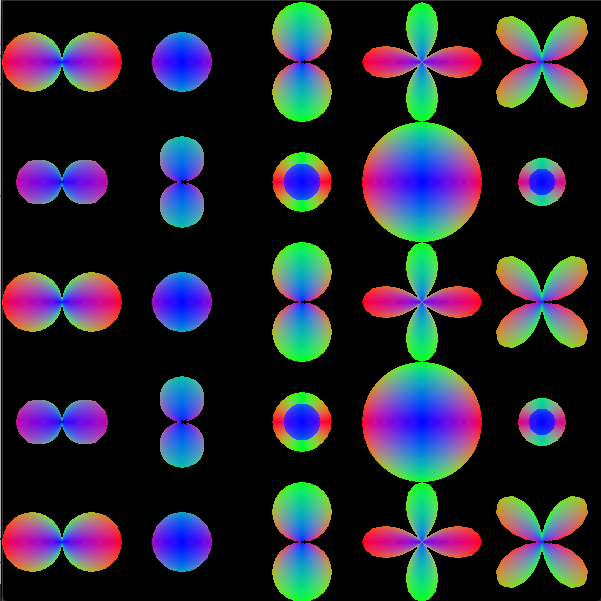
\includegraphics[width=.45\linewidth, angle=0]{figs/Renderizacao_glifos_evolucao/Ilustracao_ambiente/ambiente_5.png}
    \label{fig::ambiente_validacao_5}
    }
    \subfloat[H = 25. 625 glifos renderizados]{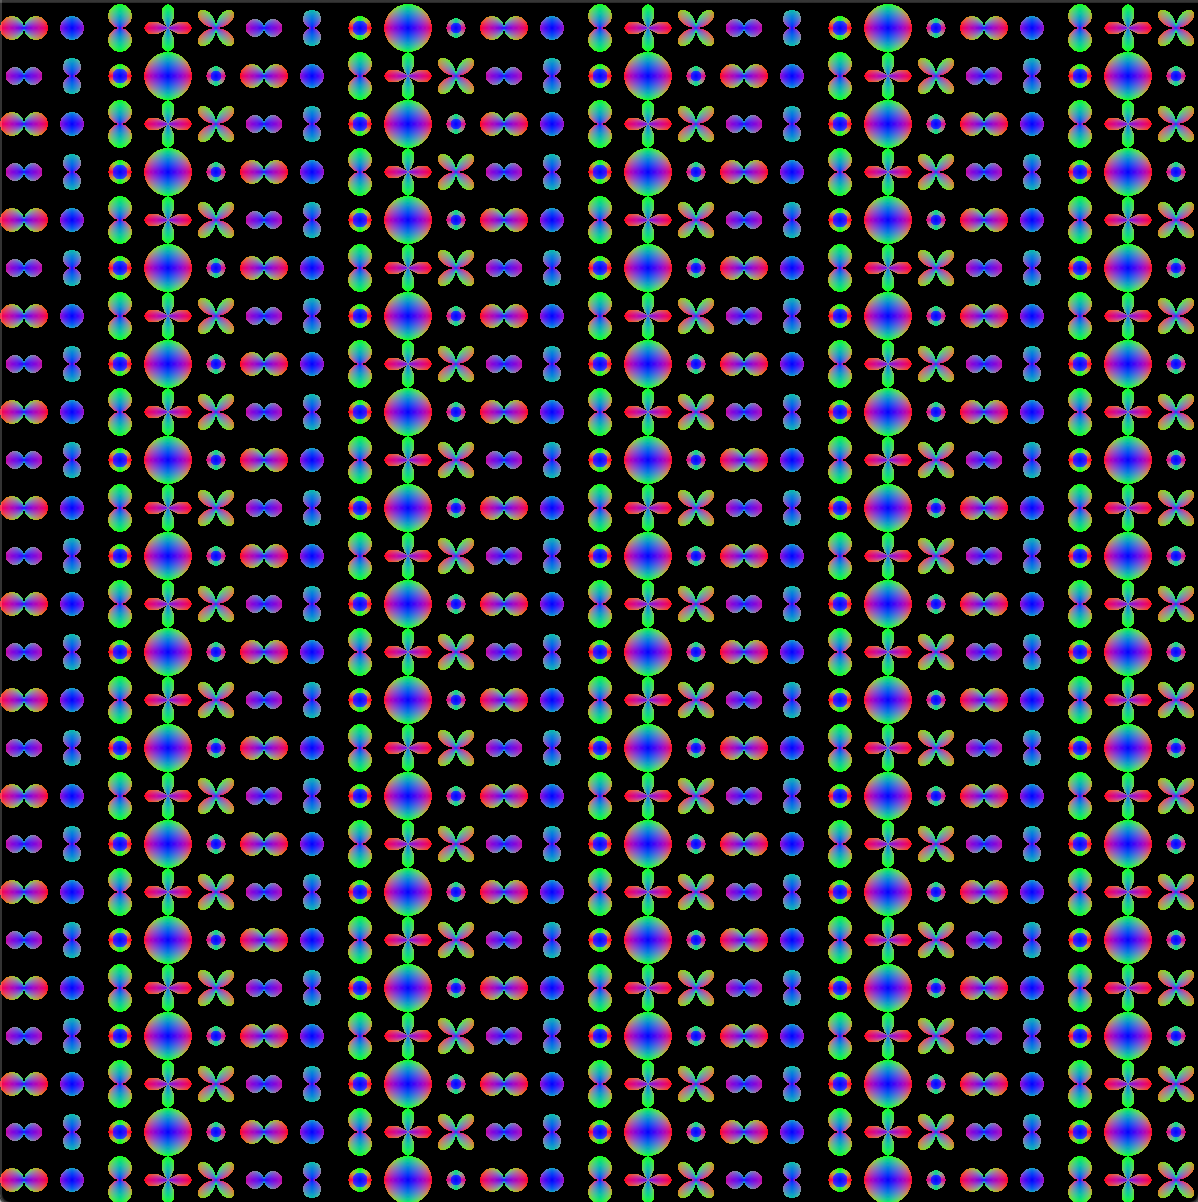
\includegraphics[width=.45\linewidth, angle=0]{figs/Renderizacao_glifos_evolucao/Ilustracao_ambiente/ambiente_25.png}
    \label{fig::ambiente_validacao_25}
    }
    
    \subfloat[H = 50. 2500 glifos renderizados]{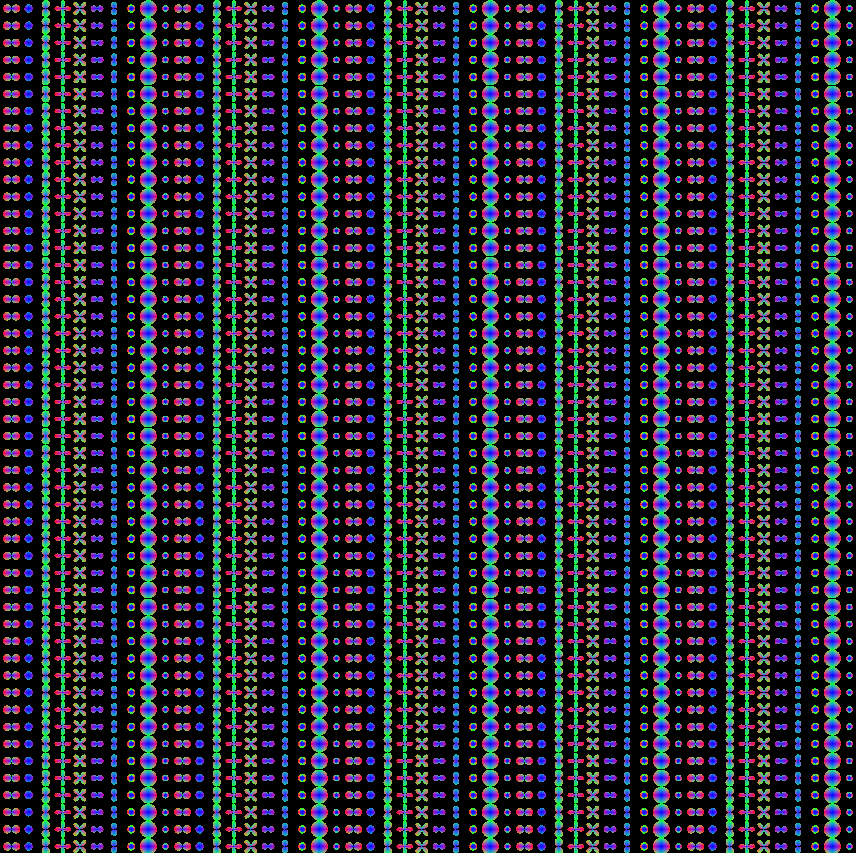
\includegraphics[width=.45\linewidth, angle=0]{figs/Renderizacao_glifos_evolucao/Ilustracao_ambiente/ambiente_50.png}
    \label{fig::ambiente_validacao_50}
    }
    \subfloat[H = 100. 10000 glifos renderizados]{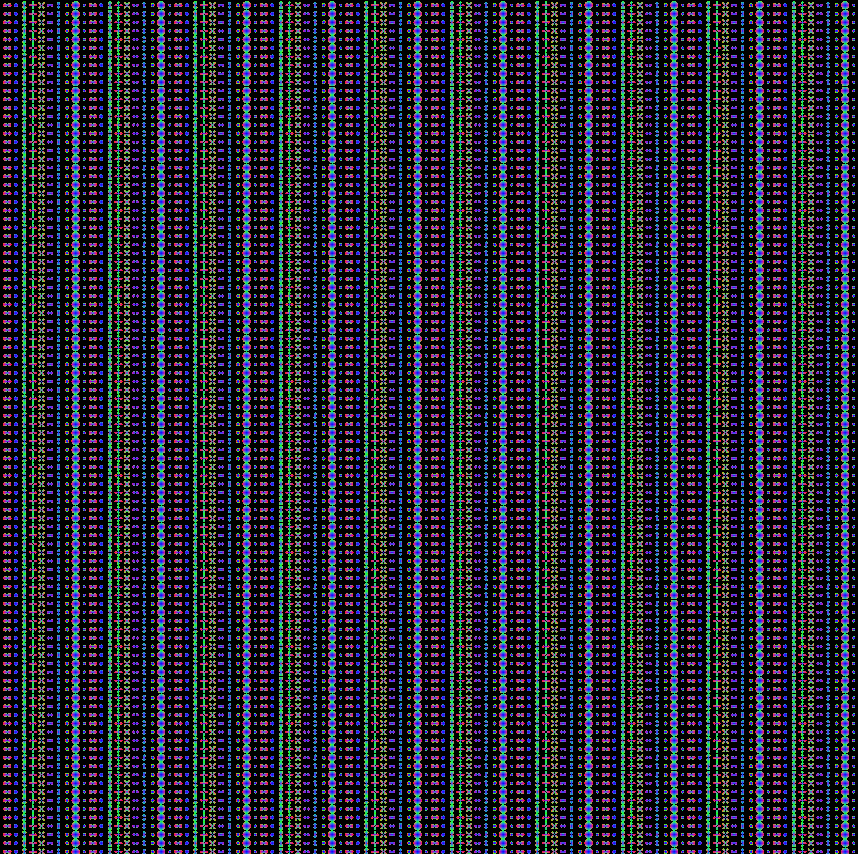
\includegraphics[width=.45\linewidth, angle=0]{figs/Renderizacao_glifos_evolucao/Ilustracao_ambiente/ambiente_100.png}
    \label{fig::ambiente_validacao_100}
    }
    %  \caption{Ambiente de teste para avaliação do algoritmo de renderização de glifos ODF}
     \caption{Renderização de glifos de ODF sintéticas em diferentes níveis de escala.}
    %\hfill
    \label{fig::ambiente_validacao}
\end{figure}

%\subsubsection{Ambiente de visualização multimodal}


Integramos o algoritmo implementado ao aplicativo VMTK-Neuro \cite{VMTKNeuro}, que renderiza os volumes anatômico co-registrados ao DWI e glifos ODF renderizados, conforme mencionado na Seção \ref{sec::superquadricas}. Sendo um ambiente de visualização multimodal, esperamos reusar todas as funcionalidades de exploração já disponíveis para avaliar a interatividade e a escalabilidade do algoritmo. O ambiente é utilizado nos experimentos nas Seções \ref{sec::multi_resolução_e_performance_em_ambiente_de visualização_multimodal} e \ref{sec::aspectos_visuais_e_interpretabilidade}.







%Esta classe de funções também é comumente utilizada pela comunidade de pesquisa de métodos de alta ordem em DWI.

\subsection{Dados de teste}
\label{ssec::dados_de_teste}

Foram utilizados dois conjuntos de dados para teste. Um conjunto compreende os dados sintetizados a partir de funções harmônicas esféricas, e outro conjunto são dados obtidos a partir de um volume de ressonância magnética disponível no repositório \textit{WU-Minn HCP Retest Data} do \textit{Connectome Project Consortium} \cite{essen2012}. Utilizamos as funções harmônicas esféricas para geração de dados sintéticos, porque os glifos destas funções são conhecidos\footnote{A página \url{https://chem.libretexts.org/@go/page/283935} oferece a visualização das funções harmônicas esféricas em plotagens polares esféricas.}. Isso serviu de suporte para depuração dos códigos.  E usamos os dados reais do \textit{Connectome Project Consortium} por ser um repositório amplamente utilizado pela comunidade e que encontramos os volumes de ressonância magnética ponderada em T1 e ponderada em difusão com alta resolução angular (HARDI) de um mesmo paciente.

%\todo[inline]{Revise o texto. \textcolor{green}{Revisado e reestruturado}}

\subsubsection{Dados sintéticos}
\label{sssec::dados_sinteticos}

 As amostras que geram os glifos no ambiente de teste são computadas a partir de ODFs derivadas de funções harmônicas esféricas, cujo grau das funções varia de zero a três. 
Indexamos as células nas quais os glifos são renderizados como $1$, $2$, ..., $M$, cuja sequência é crescente na ordem esquerda para direita e cima e para baixo, e $M = H^2$ na Fig. \ref{fig::ambiente_validacao}. Associamos o conjunto de amostras a serem renderizadas à $j$-ésima $(1 \leq j \leq M)$ célula como $\boldsymbol{R}(j) = [
R(j, \mathbf{n}_1), 
R(j, \mathbf{n}_2), 
R(j, \mathbf{n}_3), ..., 
R(j, \mathbf{n}_N)
]^T$, onde $\mathbf{n}_k$ é o vetor unitário com direção e sentido associado à normal do ponto $P_k$ de uma malha esférica $(\Pi, I_{3\tau \times 1})$ tesselada em $\Pi = [P_1, P_2, \dots, P_N]$ pontos. $I_{3\tau \times 1}$ é o conjunto de índices que triangulam $\Pi$ a fim de gerar a malha esférica de $\tau$ triângulos.%\footnote{Escolhemos esta forma de indexar as variáveis envolvidas para que fique similar à forma utilizada no Capítulo \ref{chap::renderizacao_interativa_de_perfis_de_difusao}.}

%\todo[inline]{ Na Fig 4.1.(a) há 25 glifos ... como eles correspondem às 10 funções harmônicas? \textcolor{green}{Eu associo o índice de célula ao glifo de forma periódica. Reescrevi isso para deixar de forma mais clara.}}
Utilizamos dez funções harmônicas esféricas que são repetidas periodicamente em relação às células. Nas duas primeiras linhas, na Fig. \ref{fig::ambiente_validacao_5}, da esquerda para direita e parte superior para inferior, consistem em: $Re(Y_1^{-1})$,
$Re(Y_1^0)$,
$Im(Y_1^{-1})$,
$Re(Y_2^{-2})$,
$Im(Y_2^{-2})$,
$Re(Y_2^{-1})$,
$Im(Y_2^{-1})$,
$Y_2^0$,
$Y_0^0$ e
$Y_3^0$, onde $Y_l^m$ se refere a harmônica esférica de grau $l$ e ordem $m$. O padrão de repetição das harmônicas esféricas ao índice de célula é mostrado na tabela \ref{tab::harmonicas_esfericas}.

\begin{table}[ht]
\centering
\begin{tabular}{cc}
$j \mod 10$ & Harmônica Esférica \\ \hline
1 & $Re(Y_1^{-1})$  \\
2 & $Re(Y_1^0)$     \\
3 & $Im(Y_1^{-1})$  \\
4 & $Re(Y_2^{-2})$  \\
5 & $Im(Y_2^{-2})$  \\
6 & $Re(Y_2^{-1})$  \\
7 & $Im(Y_2^{-1})$  \\
8 & $Y_2^0$         \\
9 & $Y_0^0$         \\
0 & $Y_3^0$        
\end{tabular}
\caption{Associação de índice de célula $j$ para função harmônica esférica utilizada.}
\label{tab::harmonicas_esfericas}
\end{table}

As expressões analíticas para as harmônicas esféricas de ordem zero a dois e $Y_3^0$ são:

\begin{equation}
\begin{array}{l}
Y_{0}^{0}(\theta, \varphi)=\frac{1}{2} \sqrt{\frac{1}{\pi}} \\
Y_{1}^{-1}(\theta, \varphi)=\frac{1}{2} \sqrt{\frac{3}{2 \pi}} \sin (\theta) e^{-i \varphi} \\
Y_{1}^{0}(\theta, \varphi)=\frac{1}{2} \sqrt{\frac{3}{\pi}} \cos (\theta) \\
Y_{1}^{1}(\theta, \varphi)=\frac{-1}{2} \sqrt{\frac{3}{2 \pi}} \sin (\theta) e^{i \varphi} \\
Y_{2}^{-2}(\theta, \varphi)=\frac{1}{4} \sqrt{\frac{15}{2 \pi}} \sin ^{2} (\theta) e^{-2 i \varphi} \\
Y_{2}^{-1}(\theta, \varphi)=\frac{1}{2} \sqrt{\frac{15}{2 \pi}} \sin (\theta) \cos (\theta) e^{-i \varphi} \\
Y_{2}^{0}(\theta, \varphi)=\frac{1}{4} \sqrt{\frac{5}{\pi}}\left(3 \cos ^{2} (\theta)-1\right) \\
Y_{2}^{1}(\theta, \varphi)=\frac{-1}{2} \sqrt{\frac{15}{2 \pi}} \sin (\theta) \cos (\theta) e^{i \varphi} \\
Y_{2}^{2}(\theta, \varphi)=\frac{1}{4} \sqrt{\frac{15}{2 \pi}} \sin ^{2} (\theta) e^{2 i \varphi} \\
Y_{3}^{0}(\theta, \varphi)=\frac{1}{4} \sqrt{\frac{7}{\pi}}\left(5 \cos ^{3} (\theta)-3 \cos (\theta)\right) ,
\end{array} 
\end{equation}
onde a conversão de $\mathbf{\hat{u}} = (u_x, u_y, u_z)$, $|\mathbf{\hat{u}}| = 1$, para o par $(\theta, \varphi)$ é $(\theta, \varphi)$ = ($\arccos (u_z)$, $\arctan (u_y/u_x)$).

O pré-cômputo das amostras $\boldsymbol{R}(j)$ associadas a célula de índice $j$ consiste na associação a sua respectiva harmônica esférica de acordo com a Tabela \ref{tab::harmonicas_esfericas}. Computamos o valor absoluto de cada harmônica, aplicamos nela a normalização min-max para o intervalo $[0, 1]$\footnote{No caso da harmônica esférica $(Y_0^0)$, que é constante e mapeada em um glifo esférico, normalizamos a função para ser constante igual a um.}, e o armazenamos na CPU. Fig. \ref{fig::ambiente_validacao} ilustra os glifos no ambiente de teste para diferentes valores de $M$. O cômputo do valor absoluto torna estas funções simétricas em relação aos eixos coordenados, assim como as dODFs.

%\sout{Utilizamos o ambiente de testes na série de experimentos da Seção \ref{sec::funcionalidades_agregadas_e_ganhos_de_performance}.}




\subsubsection{Dados de ressonância magnética}
\label{sssec::dados_de_ressonancia_magnetica}

%\todo[inline]{Revise o texto. \textcolor{green}{Falo o índice do volume? Ou dizer mulher 22-35 anos saudável é suficiente?}}

Utilizamos os dados do repositório \textit{WU-Minn HCP Retest Data} mantido pelo \textit{Connectome Project Consortium} \cite{essen2012}\footnote{Para os testes, não foi possível fazer aquisições segundo o protocolo HARDI com o escaneador Philips Achieva 3T disponível no hospital-universidade da Unicamp por medidas de contenção da COVID-19.}.
Os dados de difusão foram adquiridos em um \textit{scanner} Siemens 3T Skyra. A aquisição é \textit{multi-shell} com 90 gradientes de ponderação de difusão para cada \textit{shell} $b = 1000, 2000$ e $3000 s/mm^2$, estas direções são uniformemente distribuídas nos três \textit{shells}, e adicionalmente foram escaneados 6 aquisições $b0$ para cada \textit{shell}, totalizando 288 volumes. Todos os dados foram pré-processados com a \textit{pipeline} de pré-processamento do \textit{Human Connectomme Project} (HCP) \cite{glasser2013}. 

Selecionamos um volume $145\times 174\times  145$ (3.658.350 \textit{voxels}) com espaçamentos entre as amostras de $1.25\times 1.25 \times 1.25$mm$^3$. Os dados são provenientes de uma mulher saudável na faixa etária entre 22-35 anos de idade.
A aquisição anatômica ponderada em T1 do mesmo controle foi também pré-processada utilizando a \textit{pipeline} de pré-processamento do HCP \cite{glasser2013}. Como o seu respectivo DWI, é um volume $145\times 174\times  145$ (3.658.350 \textit{voxels}) com espaçamentos entre as amostras de $1.25\times 1.25\times 1.25$mm$^3$.

As dODFs foram obtidas através do GQI \cite{yeh2010} (Capítulo \ref{chapter::metodos_hardi}) e min-max normalizadas. O fator $\sigma \sqrt{6D}$ que utilizamos é de 0,0239. As amostras foram computadas com base no hemisfério da $8^{a}$ ordem de tesselação do icosaedro e armazenadas na CPU, gerando um total de 321 amostras por \textit{voxel}.

%\sout{Utilizamos estes dados nos experimentos feitos com o ambiente de visualização multimodal descritos nas Seções \ref{sec::multi_resolução_e_performance_em_ambiente_de visualização_multimodal} e \ref{sec::aspectos_visuais_e_interpretabilidade}.}

%%%%%%%%%%%%%%%%%%%%%%%%%%%%%%%%%%%%%%%%%%%%%%%%%%%%%%%%%%%%%%%
%\section{Experimentos}
%\label{sec::experimentos}

% Apresentamos os resultados do algoritmo proposto em 3 grupos de experimentos, que estão descritos nas Seções 

% O primeiro grupo de experimentos tem como objetivo validar o impacto das diferentes estratégias adotadas na renderização dos glifos ODFs, quanto à ocupação de memória, ao desempenho temporal e à escalabilidade. Foram usados os dados sintéticos no ambiente de testes. Avaliamos comparativamente as 4 diferentes configurações em que diferentes estratégias foram integradas incrementalmente: (1) técnica de indexação e visibilidade; (2) técnica de instanciação; (3) compactação de dados de difusão; e (4) coalescência.

% O segundo grupo de experimentos procura certificar a interatividade e a escalabilidade do algoritmo de renderização proposto em volumes reais. Nele iremos validar a funcionalidade de multi-resolução em função das métricas do ambiente de visualização multimodal através do tempo de resposta do sistema em relação à variação dos fatores de escala de visualização, emulando um ambiente de exploração em que um usuário possa variar a escala do que está investigando sob demanda.

% O terceiro grupo de experimentos tem como objetivo de comparar visualmente os glifos superquádricos e os glifos ODFs apresentados neste trabalho quanto à eficiência na visualização das orientações múltiplas de fibras em amostras obtidas pelo protocolo HARDI de exames de ressonância magnética ponderada em difusão.

%\todo[inline]{Com a sua reestruturação perdeu-se referências aos dados sintéticos e dados reais ... Isso é importante para avaliar o potencial clínico da sua solução ... Além disso, na apresentação dos resultados é importante incluir o planejamento de experimentos, contendo a justificativa e a expectativa! Por favor, reconsidere a sua reestruturação!}

%\todo[inline]{Preste atenção na uniformidade dos títulos e sub-títulos. Há uma grande mistura maíuscula e minúscula. \textcolor{green}{OK!}}
\section{Ganhos em desempenho}
%\section{Funcionalidades agregadas e ganhos de performance}
%\section{Funcionalidades adicionadas e ganhos de performance}
\label{sec::funcionalidades_agregadas_e_ganhos_de_performance}

Nesta seção, abordamos os experimentos que nos permitiram avaliar, quanto à complexidade de memória e de tempo, o impacto das diferentes estratégias adotadas no algoritmo de renderização de glifos ODF apresentado no Capítulo \ref{chap::renderizacao_interativa_de_perfis_de_difusao}.
Nos experimentos variamos a divisão $H$ nos eixos $x$ e $y$ da janela de exibição de 5 até 100, e a resolução de amostragem, setando a ordem de tesselação do icosaedro entre $2^a$, $4^a$, $8^a$ e $16^a$. Fig. \ref{fig::ambiente_validacao} ilustra a partição da área de janela em 25, 625, 2500 e 10000 células. A cada requisição de desenho, todos os dados de translação e que geram os glifos associados a ODFs de índices $[1, 2, 3, ..., M]$ $(M = H^2)$ e que consistem no tráfego de dados CPU-GPU são enviados à GPU, o que é demandado no ambiente de visualização multimodal, conforme mostrado no fluxograma da Fig. \ref{fig::vmtk_simplified}.

 Avaliamos comparativamente as 4 diferentes configurações em que diferentes estratégias foram integradas incrementalmente: (1) técnica de indexação e visibilidade; (2) técnica de instanciação; (3) compactação de dados de difusão; e (4) coalescência.
 

%Na Seção \ref{sec::ambiente_teste}, descrevemos o ambiente de teste que implementamos para fazer a validação  de todas as funcionalidades adicionadas no algoritmo de renderização.

%Na Seção \ref{sec::primeiro_prototipo}, descrevemos o primeiro protótipo do algoritmo, onde o utilizamos na infraestrutura do ambiente de visualização multimodal para renderização dos glifos. Inicialmente, o protótipo consistiu em uma ferramenta visual para visualização de dados de ODFs em seus respectivos \textit{voxels}.

\subsection{Descrição}
\label{ssec:exp1_descricao}

%Nesta seção, validaremos o impacto das diferentes estratégias adotadas na renderização dos glifos ODFs, quanto à ocupação de memória, ao desempenho temporal e à escalabilidade. Foram usados os dados sintéticos no ambiente de testes.

Para realizar este grupo de experimentos, desativamos as funções de instanciação, compactação de dados de difusão, coalescência e multi-resolução, e coletamos o tempo médio que se levou para renderizar. Em cada série de experimentos, fomos reativando essas funções incrementalmente, na sequência de instanciação, compactação e coalescência, para coletar o mesmo conjunto de dados para análises comparativas. Nos experimentos de cada série, a coleção do tempo médio é efetuado para os glifos gerados a partir das tesselações de ordem 2, 4, 8 e 16. Utilizamos apenas um comando de desenho em todas as séries para efetuar a renderização.

Na primeira série deste experimento, computamos em cada interação os vértices de todos os glifos na CPU, deslocando os $N$ vértices de cada malha esférica para cada um dos $M$ glifos a serem renderizados. Para melhorar o tempo de execução do algoritmo, paralelizamos o processamento utilizando a API (\textit{Application Programming Interface}) OpenMP. Após o cômputo, os $N\times M$ vértices são enviados à GPU como dados do \textit{buffer} de vértices. Sendo o deslocamento de cada glifo replicado para todos os seus vértices, as coordenadas de deslocamento são também enviadas à GPU  através do \textit{buffer} de dados de vértices. Portanto, o \textit{buffer} de dados contém $N\times M \times 6$ elementos.
Adicionalmente, um conjunto $I$ de índices de triângulos de todos os glifos, são enviados como \textit{buffer} de índices com $3\tau M$ elementos, onde $\tau$ é a quantidade de triângulos da malha. A renderização dos glifos é disparada com o comando \textit{glDrawElements}. Na GPU, o glifo é redimensionado e deslocado para sua respectiva célula. Portanto, a quantidade de números na memória alocada na CPU e enviada para GPU é:
\begin{equation}
\label{eq::mem_odfs_trafego_1.1}
    \mathscr{N} =  3\tau M + 6NM = 3M(\tau + 2N).
\end{equation}
Substituindo $N$ pela Eq. \ref{eq::icosphere_vertices} e $\tau$ pela Eq. \ref{eq::icosphere_triangulos}, podemos exprimir a quantidade de valores escalares envolvidos na representação dos dados dos $M$ glifos de nível de amostragem proveniente da subdivisão de ordem $t$ do icosaedro pela expressão:
\begin{equation}
\label{eq::mem_odfs_trafego_1.2}
    \mathscr{N} = 3M( 20\times t^2 + 2(10\times t^2 +2)) = M(120t^2 + 12).
\end{equation}
Se cada valor escalar ocupar 4 \textit{bytes}\footnote{No experimento, utilizamos pontos flutuantes para descrição dos vértices e inteiros sem sinal para índices. Ambos ocupam 4 \textit{bytes}.}, o volume de dados envolvidos em cada interação é $4M(120t^2 + 12)$ \textit{bytes}. Neste experimento, a ocupação de memória da GPU $\mathscr{G}$ para formação dos glifos é a mesma da quantidade dos dados enviados.

Na segunda série de experimentos, aplicamos a instanciação. Enviamos a malha esférica unitária e centrada na origem para GPU para ser instanciada $M$ vezes. Cada instanciação envolve $N$ vértices, um conjunto de índices de tamanho $3\tau$ e um vetor de deslocamento. Os dados de $M$ instâncias são enviados à GPU via um vetor instanciado (\textit{instanced array}). Adicionalmente, enviamos $N\times M$ escalares de ODF como uma textura 2D com apenas um canal $RED$ ativado em cada \textit{texel}. É armazenado nesse canal um elemento $R(j, \mathbf{n}_i)$, que desloca apenas um ponto $P_i$ na malha esférica instanciada. A cada requisição de desenho para $M$ glifos, via o comando \textit{glDrawElementsInstanced},
a malha esférica instanciada é deformada, redimensionada e deslocada para a sua célula na GPU. Cada $R(j, \mathbf{n}_i)$ 
é acessado no \textit{vertex shader} com as coordenadas $(Instance\_ID, Vertex\_ID)$. Com base no que foi exposto, o tráfego de dados é reduzido a:
\begin{equation}
\label{eq::mem_odfs_trafego_2.1}
    \mathscr{N} =  MN + 3M = M(N+3) = M(10 t^2 + 2 + 3) = M(10t^2 + 5),
\end{equation}
e a quantidade de dados alocados na memória da GPU envolvidos na renderização:
\begin{equation}
\label{eq::mem_odfs_ocupancia_2.1}
\begin{array}{l}
    \mathscr{G} =  (4MN + 3M) + (N + 3\tau) \\
    \mathscr{G} = 4M(10t^2+2) + 3M + 10\times t^2 + 2 + 60t^2 \\
    \mathscr{G} = M(40t^2 + 11) + 70t^2 + 2 .
    \end{array}
\end{equation}
O termo $4MN$ vem do fato de um \textit{texel} ser associado a quatro coordenadas, (\textit{R(ed), G(reen), B(lue), A(lpha)}), da textura, embora apenas o canal $R$ seja usado efetivamente para armazenar os valores de ODF neste experimento. A componente $3M$ se refere as $M$ coordenadas de translação e $(N + 3\tau)$ à malha esférica já carregada na GPU. A quantidade de memória alocada na GPU envolvida na renderização é de ($4M(40t^2 + 11) + 280t^2 + 8$) \textit{bytes}.

Na terceira série de experimentos, ao explorarmos a propriedade de simetria em relação aos eixos de $R(j, \mathbf{\hat{u}})$, podemos reduzir para metade a quantidade de amostras $R(j, \mathbf{\hat{u}})$ associadas às $N$ direções. Sugerimos manter as antípodas em posições subsequentes em memória, para facilitar acessos dos pares de antípodas ao mesmo escalar de ODF. Passamos a enviar $\frac{N}{2} \times M$ escalares de difusão como uma textura 2D com apenas um canal $RED$ para GPU. Para cada par de antípodas, o escalar de difusão correspondente é acessado pelas coordenadas $(Instance\_ID, \lfloor \frac{Vertex\_ID}{2} \rfloor)$. Em relação às configurações dos experimentos anteriores, o tráfego é reduzido para:
\begin{equation}
\label{eq::mem_odfs_trafego_3.1}
    \mathscr{N} =  M \frac{N}{2} + 3 M = M (\frac{N}{2} +3) = M(5\times t^2 + 1 + 3) = M(5t^2 + 4).
\end{equation}
A quantidade de espaço alocado na memória da GPU se torna:
\begin{equation}
\label{eq::mem_odfs_ocupancia_3.1}
\begin{array}{l}
    \mathscr{G} =  (4\times M\times \frac{N}{2} + 3\times M) + (N + 3\tau) \\
    \mathscr{G} = 4M(5t^2+1) + 3M + 10\times t^2 + 2 + 60t^2 \\
    \mathscr{G} = M(20t^2 + 7) + 70t^2 + 2 .
    \end{array}
\end{equation}
Em \textit{bytes}, a ocupação da memória da GPU é de: ($4M(20t^2 + 7) + 280t^2 + 8$).

Na quarta série do experimento, procuramos otimizar o uso da memória de textura compactando 4 amostras de $R(j, \mathbf{n}_i)$ num \textit{texel}, propiciando acessos coalescentes\footnote{Informações sobre a alocação de memória em uma textura de diferentes formatos podem ser encontradas em \url{https://www.khronos.org/registry/OpenGL-Refpages/gl4/html/glTexImage2D.xhtml}} (Seções \ref{ssec::coalescencia} e \ref{ssec::vertex_shader}). Com isso, o tráfego de dados se torna:
\begin{equation}
\label{eq::mem_odfs_trafego_4.1}
\begin{array}{l}
    \mathscr{N} =  M\times 4 \times \lceil\frac{N/2}{4}\rceil + 3M \\
    \mathscr{N} =  M( 4 \times \lceil \frac{1}{4}(5t^2 + 1)\rceil + 3) . %= M\times (\frac{N}{2} + 3).% = M(5\times t^2 + 1 + 3) = M(5t^2 + 4);
    \end{array}
\end{equation}
O termo de arredondamento para o próximo inteiro $\lceil\frac{N/2}{4}\rceil$ diz respeito às dimensões das texturas suportadas pela GPU. Caso $N/2$ não seja divisível por 4, é necessário adicionar linhas \textit{dummy} na matriz para garantir que a quantidade de elementos em cada coluna da matriz de escalares de ODF seja um múltiplo de 4. Como $t$ é uma potência de 2, $5t^2 + 1$ deixa resto 1 na divisão por quatro. O próximo número acima de $5t^2 + 1$ que é divisível por 4 é dado por $5t^2 + 4$, logo podemos afirmar que $4 \times \lceil \frac{1}{4}(5t^2 + 1)\rceil = 5t^2 + 4$. Então Eq. \ref{eq::mem_odfs_trafego_4.1} se torna:
\begin{equation}
\label{eq::mem_odfs_trafego_4.2}
\begin{array}{l}
    \mathscr{N} =  M (5t^2 + 4 + 3) = M (5t^2 + 7).
    \end{array}
\end{equation}
A quantidade de números alocados na memória com a coalescência se torna o mesmo do tráfego de dados, em adição à malha esférica e \textit{buffer} de índices já armazenados na GPU:
\begin{equation}
\label{eq::mem_odfs_ocupancia_4.1}
\begin{array}{l}
    \mathscr{G} =  \mathscr{N} + (N + 3\tau) \\
    \mathscr{G} =   M (5t^2 + 7) + 10 t^2 + 2 + 60t^2\\
    \mathscr{G} = M(5t^2 + 7) + 70 t^2 + 2 ,
    \end{array}
\end{equation}
e a quantidade total de memória alocada na GPU para renderização dos glifos é ($4M(5t^2 + 7) + 280t^2 + 8$) \textit{bytes}.


%Para evitar o desperdício de memória e mal uso do cache da GPU, enviamos $\boldsymbol{\mathscr{R}}$ como uma textura de formato RGBA, de tamanho $\lceil \frac{N/2}{4}\rceil \times M$ em que agrupamos os valores escalares da $j$-ésima coluna em sequência de quatro em quatro. Se $N/2$ não é divisível por quatro, é necessária a inserção de linhas com valores \textit{dummy} em $\boldsymbol{\mathscr{R}}$ afim de completar a divisibilidade por quatro, para que cada coluna da matriz possa ser acessada via índice de instância.

%Assim, em cada \textit{texel} há quatro amostras de ODF que escalonam 8 pontos da malha esférica. No Capítulo \ref{chap::renderizacao_interativa_de_perfis_de_difusao}, a Fig. \ref{fig::texelfetch} ilustra a forma que o \textit{lookup} é feito, onde neste contexto $j = d_j$. O argumento da função \textit{texelFetch} para a $j$-ésima instância se torna as coordenadas não-normalizadas $(j, \lfloor \frac{Vertex\_ID}{8} \rfloor)$ e o acesso do ponto processado ao seu respectivo valor de ODF min-max normalizado, considerando que as componentes R, G, B e A são mapeados nos índices 0, 1, 2 e 3 nos \textit{texels} é mapeado por $\lfloor Vertex\_ID \mod{8}/2 \rfloor$.
 
\subsection{Resultados}


%\todo[inline]{Revise o texto e, principalmente, as legendas para que fiquem coerentes com o restante do texto. Diminua um pouco os gráficos ... ou a legenda ...  Pode ser que caibam 2 figuras por página.\textcolor{green}{OK!}}

Neste primeiro grupo de experimentos, procuramos sempre diminuir a quantidade de memória utilizada da GPU para geração de glifos em relação ao experimento anterior como detalhado na Seção \ref{ssec:exp1_descricao}. Além de reduzir a complexidade de memória, o tráfego de dados CPU-GPU para geração dos glifos também diminui. Mostramos nesta seção os tempos de resposta que coletamos para avaliar quantitativamente o impacto das diferentes configurações na complexidade de tempo e na escalabilidade. A escalabilidade é uma demanda do ambiente de visualização exploratória que requer interações com os dados em escalas muito diferentes, conforme discutiremos na Seção \ref{sec::multi_resolução_e_performance_em_ambiente_de visualização_multimodal}. As medidas de tempo, em quadros por segundo, (\textit{frames per second}, FPS), e em diferentes níveis de resolução das orientações de difusão, mais especificamente em ordens de tesselação 2$^a$, 4$^a$, 8$^a$, e 16$^a$, são sintetizadas em gráficos nesta seção.
Todos os dados numéricos que geraram os resultados nos gráficos nas Fig. \ref{fig::FPS_prototipo_1}, \ref{fig::FPS_prototipo_2}, \ref{fig::FPS_prototipo_3} e \ref{fig::FPS_prototipo_4} estão anotados na Seção \ref{ap::dados_serie_experimentos_1} do apêndice.

As medidas de tempo da primeira série do experimento em função da quantidade de glifos, estão sintetizadas no gráfico da Fig. \ref{fig::FPS_prototipo_1}. As curvas em cores azul, laranja, verde e vermelha representam diferentes níveis de resolução das orientações de difusão. Elas correspondem, respectivamente, a $2^{a}$ $4^{a}$, $8^{a}$ e $16^{a}$ ordem de tesselação do icosaedro.

%\todo{Com base em quê você pode afirmar que é "mais próxima"? \textcolor{green}{Feito. Descrito as similaridades e diferenças}}

%A configuração de renderização é a mais próxima da abordagem \citeonline{shattuck2008} para renderização de glifos em fatias. A similaridade reside em que os vértices dos glifos são computados na CPU e o tráfego de dados entre CPU e GPU consistem em vértices formadores de superfície, mas enquanto na nossa abordagem, as \todo{Quais amostras? \textcolor{green}{de dODF, OK!}}amostras das ODFs já são pré-computadas e são enviadas para GPU em todas as interações, \citeonline{shattuck2008} as computa a partir de funções base e faz o envio para GPU quando há uma mudança de fatia, resolução do glifo e a quantidade de funções base utilizadas feitas pelo usuário.

\begin{figure}[ht]
    \centering
    %\rule{6cm}{3cm}
    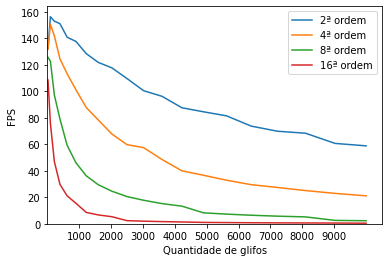
\includegraphics[width=.65\linewidth, angle=0]{figs/Renderizacao_glifos_evolucao/FPS_prototipo1_Geral_legendado.png}
    \caption{FPS $\times$ quantidade de glifos renderizada com a configuração básica, sem otimização, correspondente à primeira série de experimentos descrita na Seção \ref{ssec:exp1_descricao}.}
    \label{fig::FPS_prototipo_1}
\end{figure}

Fig. \ref{fig::FPS_prototipo_2} mostra de forma comparativa as medidas de tempo, em FPS, da configuração de renderização da segunda série de experimento, em linha azul, em relação à primeira série, em linha preta (Fig. \ref{fig::FPS_prototipo_1}).

\begin{figure}[ht]
\centering
\captionsetup[subfloat]{farskip=5pt , nearskip=0pt}
    \subfloat[Tesselação de $2^a$ ordem] {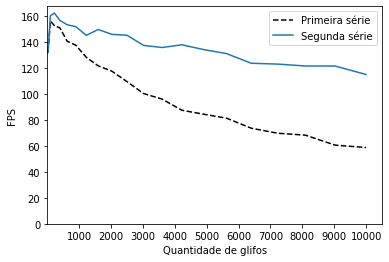
\includegraphics[width=.35\linewidth, angle=0] {figs/Renderizacao_glifos_evolucao/Prototipo2_leg/prototipo_2_42.png}
    \label{fig::FPS_prototipo_2_42}
    }
    \subfloat[Tesselação de $4^a$ ordem] {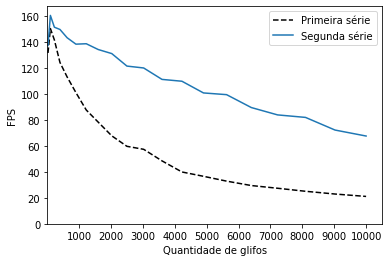
\includegraphics[width=.35\linewidth, angle=0]{figs/Renderizacao_glifos_evolucao/Prototipo2_leg/prototipo_2_162.png}
    \label{fig::FPS_prototipo_2_162}
    }
    
    \subfloat[Tesselação de $8^a$ ordem] {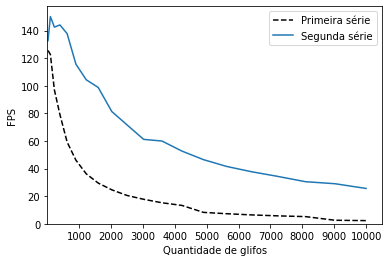
\includegraphics[width=.35\linewidth, angle=0]{figs/Renderizacao_glifos_evolucao/Prototipo2_leg/prototipo_2_642.png}
    \label{fig::FPS_prototipo_2_642}
    }
    \subfloat[Tesselação de $16^a$ ordem] {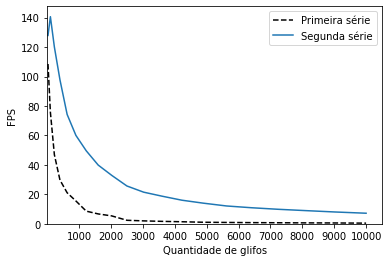
\includegraphics[width=.35\linewidth, angle=0]{figs/Renderizacao_glifos_evolucao/Prototipo2_leg/prototipo_2_2562.png}
    \label{fig::FPS_prototipo_2_2562}
    }
     \caption{FPS médio $\times$ Quantidade de glifos renderizados com a configuração da segunda série de experimentos em relação à primeira, descritas na Seção \ref{ssec:exp1_descricao}.}
    %\hfill
    \label{fig::FPS_prototipo_2}
\end{figure}

Fig. \ref{fig::FPS_prototipo_3} traz de forma comparativa o gráfico de desempenho do algoritmo de renderização configurada para a terceira série de experimentos, em linha vermelha, em relação à segunda série, em linha azul.

\begin{figure}[H]
\centering
\captionsetup[subfloat]{farskip=5pt,nearskip=0pt}
    %!!VER SE ISSO TA CERTO
    \subfloat[Tesselação de $2^a$ ordem] {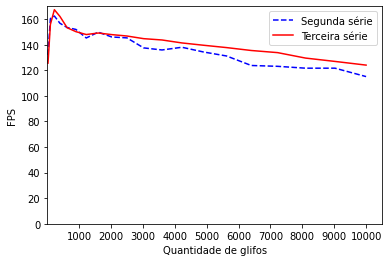
\includegraphics[width=.35\linewidth, angle=0]{figs/Renderizacao_glifos_evolucao/Prototipo3_leg/prototipo_3_42.png}
    \label{fig::FPS_prototipo_3_42}
    }
    \subfloat[Tesselação de $4^a$ ordem] {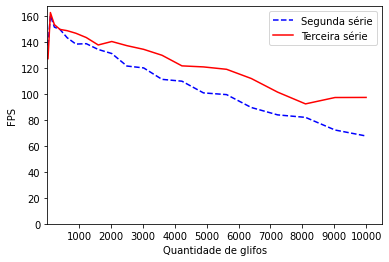
\includegraphics[width=.35\linewidth, angle=0]{figs/Renderizacao_glifos_evolucao/Prototipo3_leg/prototipo_3_162.png}
    \label{fig::FPS_prototipo_3_162}
    }
    
    \subfloat[Tesselação de $8^a$ ordem] {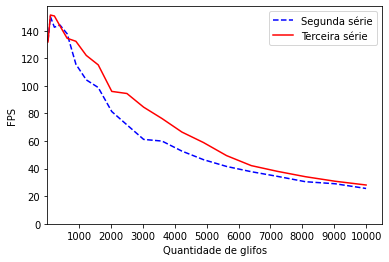
\includegraphics[width=.35\linewidth, angle=0]{figs/Renderizacao_glifos_evolucao/Prototipo3_leg/prototipo_3_642.png}
    \label{fig::FPS_prototipo_3_642}
    }
    \subfloat[Tesselação de $16^a$ ordem] {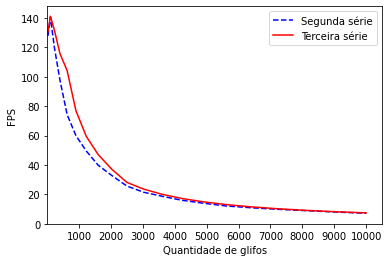
\includegraphics[width=.35\linewidth, angle=0]{figs/Renderizacao_glifos_evolucao/Prototipo3_leg/prototipo_3_2562.png}
    \label{fig::FPS_prototipo_3_2562}
    }
     \caption{FPS médio $\times$ Quantidade de glifos renderizados com a configuração da terceira série de experimentos em relação à segunda série, descritas na Seção \ref{ssec:exp1_descricao}.
     }
    %\hfill
    \label{fig::FPS_prototipo_3}
\end{figure}

Fig. \ref{fig::FPS_prototipo_4} traz de forma comparativa a taxa de quadros, em FPS, gerados pela renderização configurada para a quarta série dos experimentos, em linha magenta, em comparação à terceira série, em linha vermelha.

\begin{figure}[H]
\centering
\captionsetup[subfloat]{farskip=5pt,nearskip=0pt}
    %!!VER SE ISSO TA CERTO
    \subfloat[Tesselação de $2^a$ ordem] {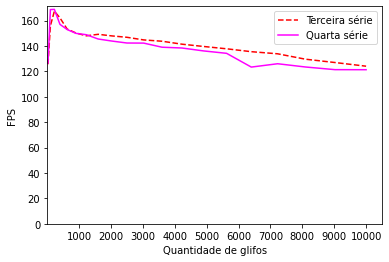
\includegraphics[width=.35\linewidth, angle=0]{figs/Renderizacao_glifos_evolucao/Prototipo4_leg/prototipo_4_42.png}
    \label{fig::FPS_prototipo_4_42}
    }
    \subfloat[Tesselação de $4^a$ ordem] {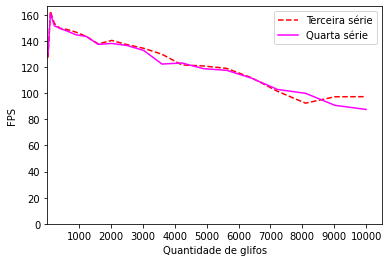
\includegraphics[width=.35\linewidth, angle=0]{figs/Renderizacao_glifos_evolucao/Prototipo4_leg/prototipo_4_162.png}
    \label{fig::FPS_prototipo_4_162}
    }
    
    \subfloat[Tesselação de $8^a$ ordem] {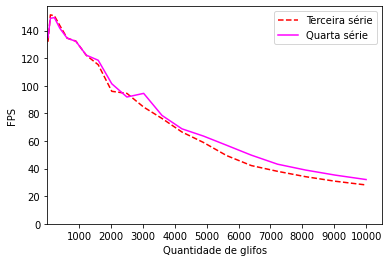
\includegraphics[width=.35\linewidth, angle=0]{figs/Renderizacao_glifos_evolucao/Prototipo4_leg/prototipo_4_642.png}
    \label{fig::FPS_prototipo_4_642}
    }
    \subfloat[Tesselação de $16^a$ ordem] {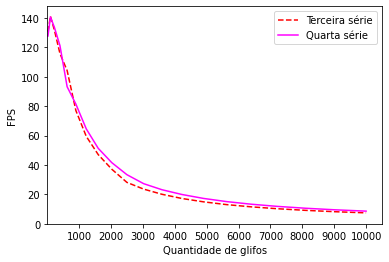
\includegraphics[width=.35\linewidth, angle=0]{figs/Renderizacao_glifos_evolucao/Prototipo4_leg/prototipo_4_2562.png}
    \label{fig::FPS_prototipo_4_2562}
    }
     \caption{FPS médio $\times$ Quantidade de glifos renderizados com a configuração da quarta série de experimentos em relação à terceira série, descritas na Seção \ref{ssec:exp1_descricao}.}
    %\hfill
    \label{fig::FPS_prototipo_4}
\end{figure}

\subsection{Discussões}

%\todo[inline]{Revise e adicione comentários sobre escalabilidade para que faça sentido as medidas de tantos números de glifos. \textcolor{green}{OK!}}

As estratégias para minimização de ocupação de memória de GPU e de redução de tráfego de dados tem como objetivo a propiciar o desenvolvimento de um ambiente exploratório da difusão intravoxel revelada pelos exames de ressonância magnética ponderada em difusão. No ambiente de visualização multimodal do VMTK-Neuro \cite{VMTKNeuro} é possível explorar exames de diferentes modalidades alinhadas, ou co-registradas, em diferentes níveis de escala. Quando diminuímos o fator de escala da imagem, aumentamos a quantidade de \textit{voxels} detectados, implicando em uma alta demanda de glifos a serem renderizados, podendo incorrer em um alto tráfego de dados e uso da memória da GPU.

%Na Seção \ref{sec::adaptatividade_de_resolucao}, introduzimos a adaptabilidade na resolução como uma função da máxima quantidade de \textit{pixels} contidos em um único \textit{voxel}, o que é algo intrínseco à métricas do ambiente de visualização multimodal. A validação da inserção deste tópico está nos resultados mostrados na Tabela \ref{tab::glyph_info_experiment}, no qual comparamos com o algoritmo de renderização de glifos ODF integrado ao ambiente de visualização multimodal onde a resolução dos glifos é fixa e derivada da $8^a$ ordem de tesselação do icosaedro, que está anotada na Tabela \ref{tab::glyph_info_experiment_fixed}.

%As medições foram feitas em um computador Macbook Pro Retina 13', com processador Intel Core i5 Dual-Core 2.7GHz, processador gráfico integrado Intel Iris Graphics 6100 1536 MB e memória RAM de 8 GB 1867 MHz DDR3. 
A configuração de renderização na primeira série dos experimentos gera um tráfego de dados excessivo entre CPU-GPU. Observe que a quantidade de dados por glifo consiste em $4(120t^2 + 12)$ \textit{bytes}. Adicionalmente, há uma redundância excessiva na quantidade de dados, como dados simétricos de uma dODF discreta e deslocamentos dos vértices. Porém, paralelizando o cômputo de deslocamentos dos vértices com uso de OpenMP, foi possível obter uma taxa de quadros razoável com as subdivisões de $2^a$ e $4^a$ ordem como ilustra a Fig. \ref{fig::FPS_prototipo_1}.

Na segunda série de experimentos, os deslocamentos dos vértices das malhas esféricas instanciadas são computados de forma paralela pelo \textit{vertex shader}. Para cada glifo, $N$ valores escalares de $R(j, \mathbf{\hat{u}})$ são enviados para GPU. Porém, os dados de deslocamento comuns a todos os vértices de um glifo e o conjunto dos índices dos vértices são passados somente uma única vez. O tráfego CPU-GPU por glifo cai de $4(120t^2 + 12)$ para $4(10t^2 + 5)$ \textit{bytes}, o que consiste em menos de $10\%$ do tráfego da primeira série de experimentos para as tesselações de ordem 2, 4, 8 e 16. A ocupação de memória na GPU pode se tornar significativamente menor quando se aumenta a quantidade de glifos renderizados. Em todas as tesselações, para mais de 100 glifos renderizados, a ocupação cai para entre 30\% e 35\% em comparação à primeira série de experimentos. No gráfico da Fig. \ref{fig::FPS_prototipo_2}, o FPS mais que dobra para milhares de glifos renderizados para $8^a$ e $16^a$ ordem de tesselação. Observe também que conseguimos renderizar mais de 3000 glifos em taxas interativas \cite{nielsen1994} a partir da malha suave gerada pela $16^a$ ordem de tesselação do icosaedro. Renderização por instâncias foi um ponto crucial neste trabalho rumo à interatividade.

Para a configuração da terceira série de experimentos exploramos a simetria em relação aos eixos das funções para reduzir o tráfego de dados para metade dos escalares de ODF.
Observe que esta otimização faz o tráfego de dados CPU-GPU ser reduzido de $4(10t^2 + 5)$  para $4(5t^2 + 4)$ \textit{bytes}, totalizando uma queda de aproximadamente $50\%$, o que também ocorre na ocupação de memória na GPU. Em termos de desempenho, observe em Fig. \ref{fig::FPS_prototipo_3_642} e \ref{fig::FPS_prototipo_3_2562} que aproximadamente 4900 e 1225 glifos puderam ser renderizados a 60 FPS para $8^a$ e $16^a$ ordem de tesselação, enquanto na abordagem em que não tomamos vantagem da simetria, 3600 e 900 puderam ser gerados. Adicionalmente, os maiores ganhos de desempenho ocorrem na faixa que compreendem 600 a 1600 glifos para $16^a$ ordem de tesselação e 2400 até 5000 glifos para $8^a$ ordem e os ganhos em FPS são acima de 20\% em comparação à abordagem anterior. Esses resultados evidenciam a relevância em tirar vantagem da propriedade de simetria das funções dODFs para aumentar o ganho mo desempenho.

Para configuração da quarta série, objetivamos reduzir a ocupação da memória da GPU para renderização dos glifos. Vimos na derivação da Eq. \ref{eq::mem_odfs_ocupancia_4.1} que, ao compactarmos 4 escalares de difusão num único \textit{texel}, reduzimos a quantidade de memória de textura alocada na GPU por um fator de aproximadamente 4. Porém, para complementar a quantidade de escalares em um múltiplo de 4, precisamos adicionar 3 escalares \textit{dummy} por glifo para as ordens de tesselação que adotamos (Eq. \ref{eq::mem_odfs_trafego_4.2}). Para mais de 100 glifos renderizados, a memória total alocada na GPU é menor que $30\%$ em relação à terceira série para as tesselações de ordem 4, 8 e 16. Tende a ser menor quando mais glifos são renderizados. Em relação ao ganho em desempenho, a variação é muito sutil. Há somente um aumento em FPS quando milhares de glifos são renderizados a partir das malhas da $8^a$ e $16^a$ ordem de subdivisão. Na subdivisão de ordem 8, o ganho em FPS é acima de 10\% para mais de 5600 glifos. %\sout{Por outro lado, a diferença é desprezível quando a quantidade de glifos renderizados é menor que 1000 para estas malhas e totalmente desprezível quando utilizamos as tesselações de ordem dois e quatro.}

%\todo[inline]{Não entendi a finalidade do parágrafo abaixo. Não seria mais interessante tecer alguns comentários em relação à interatividade e escalabilidade, tomando como base a Fig. 4.5. Pode-se mostrar que o desempenho é interativo quando a quantidade de orientações de difusão se limita em até 4$^a$ ordem e há uma drástica redução no desempenho para as 8$^a$ e 16$^a$ quando se aumenta a quantidade de glifos renderizados. Por outro lado, a baixa resolução das orientações de difusão pode tornar glifos pouco representativos em análises mais detalhadas ... Sugiro que, para mostrar a redução da capacidade informativa, ilustre um mesmo glifo com dois ou mais pares de pontas em 4 diferentes escalas. \textcolor{green}{OK!}}

Os resultados na quarta série mostram que o desempenho da renderização dos glifos é interativo com alta escalabilidade para as tesselações de ordem 2 e 4 do icosaedro, nas quais renderizamos dez mil glifos acima de 60 FPS. Por outro lado, há uma drástica redução em desempenho para tesselações de 8$^a$ e 16$^a$ ordem quando aumentamos a quantidade de glifos renderizados, porém com uma resolução maior. Fig. \ref{fig::sh_glifo_odf} ilustra o aspecto visual do glifo ODF de uma harmônica esférica para as diferentes malhas utilizadas no experimento, o que ilustra capacidade informativa dos glifos em diferentes resoluções.

\begin{figure}[H]
\centering
%\captionsetup[subfloat]{farskip=0pt,nearskip=0pt}
    %\rule{6cm}{3cm}
    \subfloat[$2^a$ ordem]{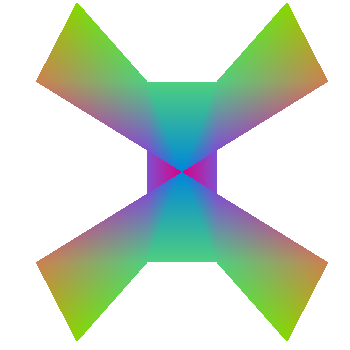
\includegraphics[width=.20\linewidth, angle=0]{figs/Esquema_Glifo/Visual/Glifos_SH/SH_42.png}
    \label{fig::sh_42}
    }
    \subfloat[$4^a$ ordem] {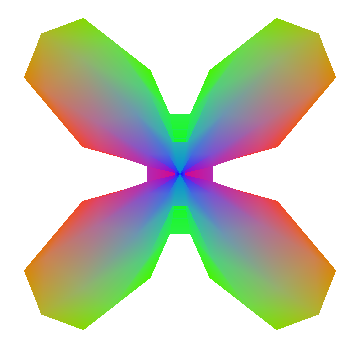
\includegraphics[width=.20\linewidth, angle=0]{figs/Esquema_Glifo/Visual/Glifos_SH/SH_162.png}
    \label{fig::sh_162}
    }
    \\
    \subfloat[$8^a$ ordem]{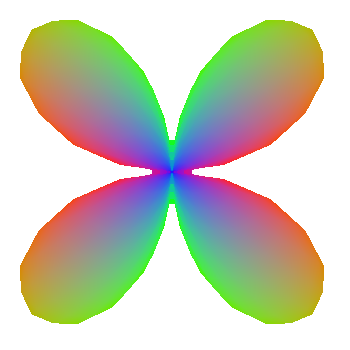
\includegraphics[width=.20\linewidth, angle=0]{figs/Esquema_Glifo/Visual/Glifos_SH/SH_642.png}
    \label{fig::sh_642}
    }
    \subfloat[$16^a$ ordem] {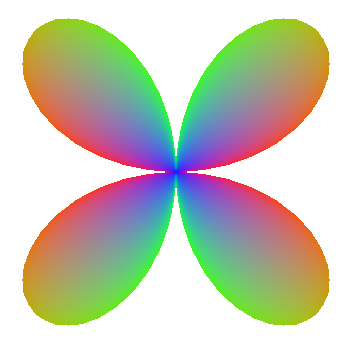
\includegraphics[width=.20\linewidth, angle=0]{figs/Esquema_Glifo/Visual/Glifos_SH/SH_2562.png}
    \label{fig::sh_2562}
    }
    \caption{Glifos ODF da parte imaginária da harmônica esférica $Y_2^{-2}$ em diferentes ordens de tesselação do icosaedro.}
    \label{fig::sh_glifo_odf}
\end{figure}



%\textcolor{magenta}{Para finalizar, compararemos os resultados da quarta série com a primeira. Em nossa proposta, conseguimos desenhar os mesmos glifos com um tráfego entre CPU-GPU e ocupação na memória da GPU em torno de \todo{Só 5\%? Nas discussões anteriores não seriam mais?}$5\%$ em comparação à quantidade de dados da primeira série do experimento para as tesselações de ordem 2, 4, 8 e 16. Adicionalmente, as deformações na superfície esférica são feitas de forma paralela na GPU em uma malha esférica instanciada. A diferença em FPS entre ambas é notória, especialmente quando usamos tesselações de oitava e décima sexta ordem e renderizamos muitos glifos. O ganho em FPS é mais de cinco vezes maior para mais de 900 glifos renderizados quando utilizamos as tesselações de oitava e décima sexta ordem (Tabela \ref{tab::testes_8} e \ref{tab::testes_16}).}

%Adicionalmente, as componentes R, G, B e A na memória de textura em cada \textit{texel} estão em sequência na GPU e nesta abordagem, as amostras que sintetizam o glifo estão espaçadas em 3 \textit{floats}. Neste leiaute de memória, no qual os coeficientes de ODF não estão em sequência, alocamos memória em excesso da GPU para valores não utilizados (componentes B, G e A de cada \textit{texel}) e não utilizamos o cache da GPU de forma ótima. Observa-se que 

% Na subdivisão de ordem 16, o ganho de FPS é cerca de 10\% para 1600 glifos renderizados e se estabiliza na faixa de 15\% para mais de 5600 glifos renderizados.


\section{Multi-resolução}
%\section{Multi-resolução e desempenho em ambiente de visualização multimodal}
\label{sec::multi_resolução_e_performance_em_ambiente_de visualização_multimodal}

Neste grupo de experimentos avaliamos o potencial do algoritmo de renderização proposto na implementação de um ambiente de visualização investigativa, sob diferentes fatores de escala, das amostras de difusão intravoxel dos exames imagiológicos. Validaremos a  multi-resolução adaptativa proposta, tanto em tempos de resposta quanto na capacidade informativa. Verificaremos o impacto da multi-resolução no compromisso entre a interatividade e a qualidade informativa dos glifos.

%Elaboramos um experimento em que coletamos os tempos médios de renderização de uma mesma cena variando apenas os fatores de escala de visualização para analisarmos a capacidade adaptativa do algoritmo e validarmos a funcionalidade de multi-resolução a diferentes fatores de escala e o seu efeito tanto em tempos de resposta quanto na qualidade dos glifos visualizados.




%\todo[inline]{Revise o texto. Para este experimento, proponho analisar a relação fator de escala (número de glifos) $\times$ tempo. \textcolor{green}{OK!}}



%\todo[inline]{Qual ângulo de visão do volume foi selecionado para testes? \textcolor{green}{axial. OK!}}



\subsection{Descrição}

%\subsubsection{Multi-resolução: performance e aspectos visuais}

%Nesta série de experimentos, validaremos a funcionalidade de multi-resolução e faremos medições de performance no ambiente de visualização multimodal.

%\todo[inline]{Para efeito comparativo, deve-se procurar variar somente o argumento que está sendo comparado ... Não entendo por quê usar 86,5 num conjunto de dados e 92,27 no outro conjunto ... Isso não é científico! \textcolor{green}{Resolvido!}}

No primeiro experimento, objetivamos averiguar o desempenho do algoritmo proposto integrado no ambiente de visualização multimodal de neuroimagens VMTK-Neuro \cite{VMTKNeuro}, conforme detalhado na Seção \ref{sec::superquadricas}. Configuramos a ordem de tesselação na $8^a$ ordem do icosaedro\footnote{Vale ressaltar aqui que, por falta de memória RAM no computador de teste para armazenar os dados referentes aos dois volumes de ressonância magnética, não pudemos fazer testes de forma plena incluindo a resolução correspondente à tesselação de ordem 16 do icosaedro.} e desabilitamos o cômputo da cobertura máxima de um \textit{voxel} na tela em \textit{pixels} $max_p$. Em uma janela de tamanho fixo $850 \times 850$, variamos o fator de escala de 1,59 para 91,05, fazendo o número de glifos renderizados variar entre 13205 e 12. Para cada fator de escala, computamos o tempo de resposta em FPS.

No segundo experimento, aplicamos o algoritmo proposto no Capítulo \ref{chap::renderizacao_interativa_de_perfis_de_difusao}: habilitamos o cômputo de $max_p$ e usamos o modelo de escolha da resolução do glifo, apresentado na Seção \ref{malha_esferica}. Da mesma forma como no primeiro experimento, em uma janela de tamanho fixo $850 \times 850$, variamos o fator de escala de 1,59 para aproximadamente 91,05 e estimamos o tempo de resposta em FPS. Registramos para cada tempo de resposta a resolução da malha esférica selecionada automaticamente. Espera-se que, maior o fator de escala, menor a quantidade de glifos e maior é a ocupação dos \textit{voxels} na tela. A resolução dos glifos tende a aumentar para preservar a qualidade da imagem dos glifos.

%Mostraremos comparativamente as fatias com os glifos, renderizados a um fator de escala de 1,59 e 13205 glifos,  em resolução fixa e em multi-resolução. Adicionalmente, mostraremos também o conjunto de glifos na mesma fatia gerados a partir do icosaedro, malha na qual não utilizamos no modelo multi-resolução.

%\todo[inline]{Não entendi o objetivo do terceiro experimento, pois parece-me que ele não faz sentido. No seu caso não é nada suave a transição de uma ordem para outra, porque as qtdes de amostras variam muito. Não sei se você percebeu que o que estamos fazendo é explorar a falha da visão humana em distinguir detalhes à distância ... }
%\sout{No terceiro experimento, objetivamos evidenciar de forma visual o limiar de transição entre malhas que geram os glifos, modificando por uma sutil mudança de fator de escala do volume de ressonância. Fixamos o tamanho da janela de saída em $500 \times 500$ para que a transição ocorra com poucos glifos renderizados e manipulamos o ambiente para que $max_p$ fique próximo do limiar de mudança de resolução da malha geradora do glifo entre a $4^a$ e $ 8^a$ ordem de tesselação para podermos aferir se a mudança de resolução é notável para o usuário.}

%\todo[inline]{Por quê não manter as mesmas condições do segundo experimento? Por quê reduzir a janela para $500 \times 500$? \textcolor{green}{Para que a transição aconteça com poucos glifos} E só ver uma transição? \textcolor{green}{Há duas transições, que é de $2^a$ para $4^a$ e $4^a$ para $8^a$. A transição da segunda para quarta acontece com muitos glifos renderizados} O ideal não seria avaliar a faixa em que o sue algoritmo suporta?}

%\todo[inline]{Não deveria ser o terceiro? 
%\textcolor{green}{reestruturado}}.%\textcolor{magenta}{segundo} experimento consiste em manipular o ambiente para que o fator de escala seja tal que $max_p$ esteja próximo do limiar de mudança entre a tesselação de $4^a$ e $ 8^a$ ordem para podermos aferir se a mudança de resolução é notável para o usuário. A resolução da janela utilizada para este experimento foi de $500 \times 500$.



%\todo[inline]{Revise o texto: Como você gerou dODFs a partir de DWIs? \textcolor{green}{Explicado na seção de dados} Quais volumes que você selecionou do repositório do consórcio? \textcolor{green}{Coloco índice do volume? Dizer que mulher saudável 22-35 anos é suficiente?} Como você planejou o experimento para analisar o desempenho em tempo e a qualidade dos glifos em mostrar as múltiplas configurações de fibras em voxels. \textcolor{green}{Performance e multi resolução estão na seção 4.4. Aspectos visuais de cruzamento e coexistecia de fibras em mesmo voxel, Seção 4.5}}

%As dODFs foram obtidas através do GQI \cite{yeh2010} (Capítulo \ref{chapter::metodos_hardi}) e min-max normalizadas. O fator $\sigma \sqrt{6D}$ que utilizamos é de 0,0239. As amostras foram computadas com base no hemisfério da $8^{a}$ ordem de tesselação do icosaedro e armazenadas na CPU, gerando um total de 321 amostras por \textit{voxel}.


\subsection{Resultados}
\label{ssec::reais_resultados}

%\todo[inline]{Revise o texto. Eu tentaria uniformizar o contexto das imagens para que se possa desenvolver uma linha de raciocínio em cima de mesmos objetos. \textcolor{green}{Revisei essa parte. Coloquei as duas imagens da multi-resolução juntas no mesmo experimento. Agora está mais coerente.}}

%\todo[inline]{Eu mostraria o conteúdo da janela e geraria imagens de mesmo tamanho.\textcolor{green}{ Coloquei. Falei que a imagem é gerada com o fator 1.51. } }

Fig. \ref{fig::fps_fatorescala} mostra as medições de FPS em função do fator de escala para os glifos renderizados com a resolução fixa, correspondente à tesselação de $8^a$  ordem (Experimento 1), e com a resolução adaptativa (Experimento 2). Anotamos no gráfico, próximo aos pontos de amostragem, a quantidade de glifos renderizadas para cada fator de escala. Essa quantidade é a mesma para ambos os experimentos em cada fator de escala. Por clareza, colocamos a quantidade de glifos renderizados abaixo da curva com o menor FPS para um dado fator de escala.

\begin{figure}[H]
    \centering
    %\rule{6cm}{3cm}
    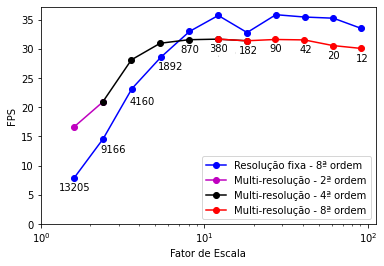
\includegraphics[width=.65\linewidth, angle=0]{figs/Esquema_Glifo/Visual/FPS_fator_de_escala_legendado_2.png}
    \caption{FPS médio $\times$ fator de escala renderizados com a resolução fixa (linha azul) e com a multi-resolução (linha multi-cores). A quantidade de glifos renderizados para cada fator de escala é mostrada próximo aos pontos de medição.}
    \label{fig::fps_fatorescala}
\end{figure}

%\todo[inline]{Fig. \ref{fig::qualidade_visual_longe_lowres} e \ref{fig::qualidade_visual_longe_highres} não são capazes de demonstrar a qualidade da informação que os glifos possam carregar!}

Para avaliar a qualidade das imagens dos glifos renderizados quanto ao poder informativo, fizemos uso do ambiente interativo do VMTK-Neuro para explorar as imagens dos glifos em diferentes níveis de escala. A Fig. \ref{fig::qualidade_visual_longe_lowres} ilustra a imagem gerada para um fator de escala de 1,59, contendo 13205 \textit{voxels} visíveis com malhas esféricas tesseladas em $2^a$ ordem de tesselação do icosaedro. Enquanto a Fig. \ref{fig::multimodal_glifo_odf_zoom} apresenta a imagem gerada para um fator de escala de 91,05, possuindo apenas 12 \textit{voxels} visíveis com malhas esféricas tesseladas em  $8^a$ ordem de tesselação do icosaedro. Note a forma dos glifos para cada nível de resolução destacada no canto esquerdo superior das Figs. \ref{fig::qualidade_visual_longe_lowres},  \ref{fig::qualidade_visual_longe_highres} e \ref{fig::qualidade_visual_longe_lowres_0}.

%%%%%%%%%%AQUI
%\todo[inline]{Selecione um glifo interessante nas Figs. 4.7 e 4.9 e coloque num dos 4 cantos da figura a sua imagem bem destacada. \textcolor{green}{OK!}}

 \begin{figure}[H]
 %\subfigcapskip = -5pt
     \centering
     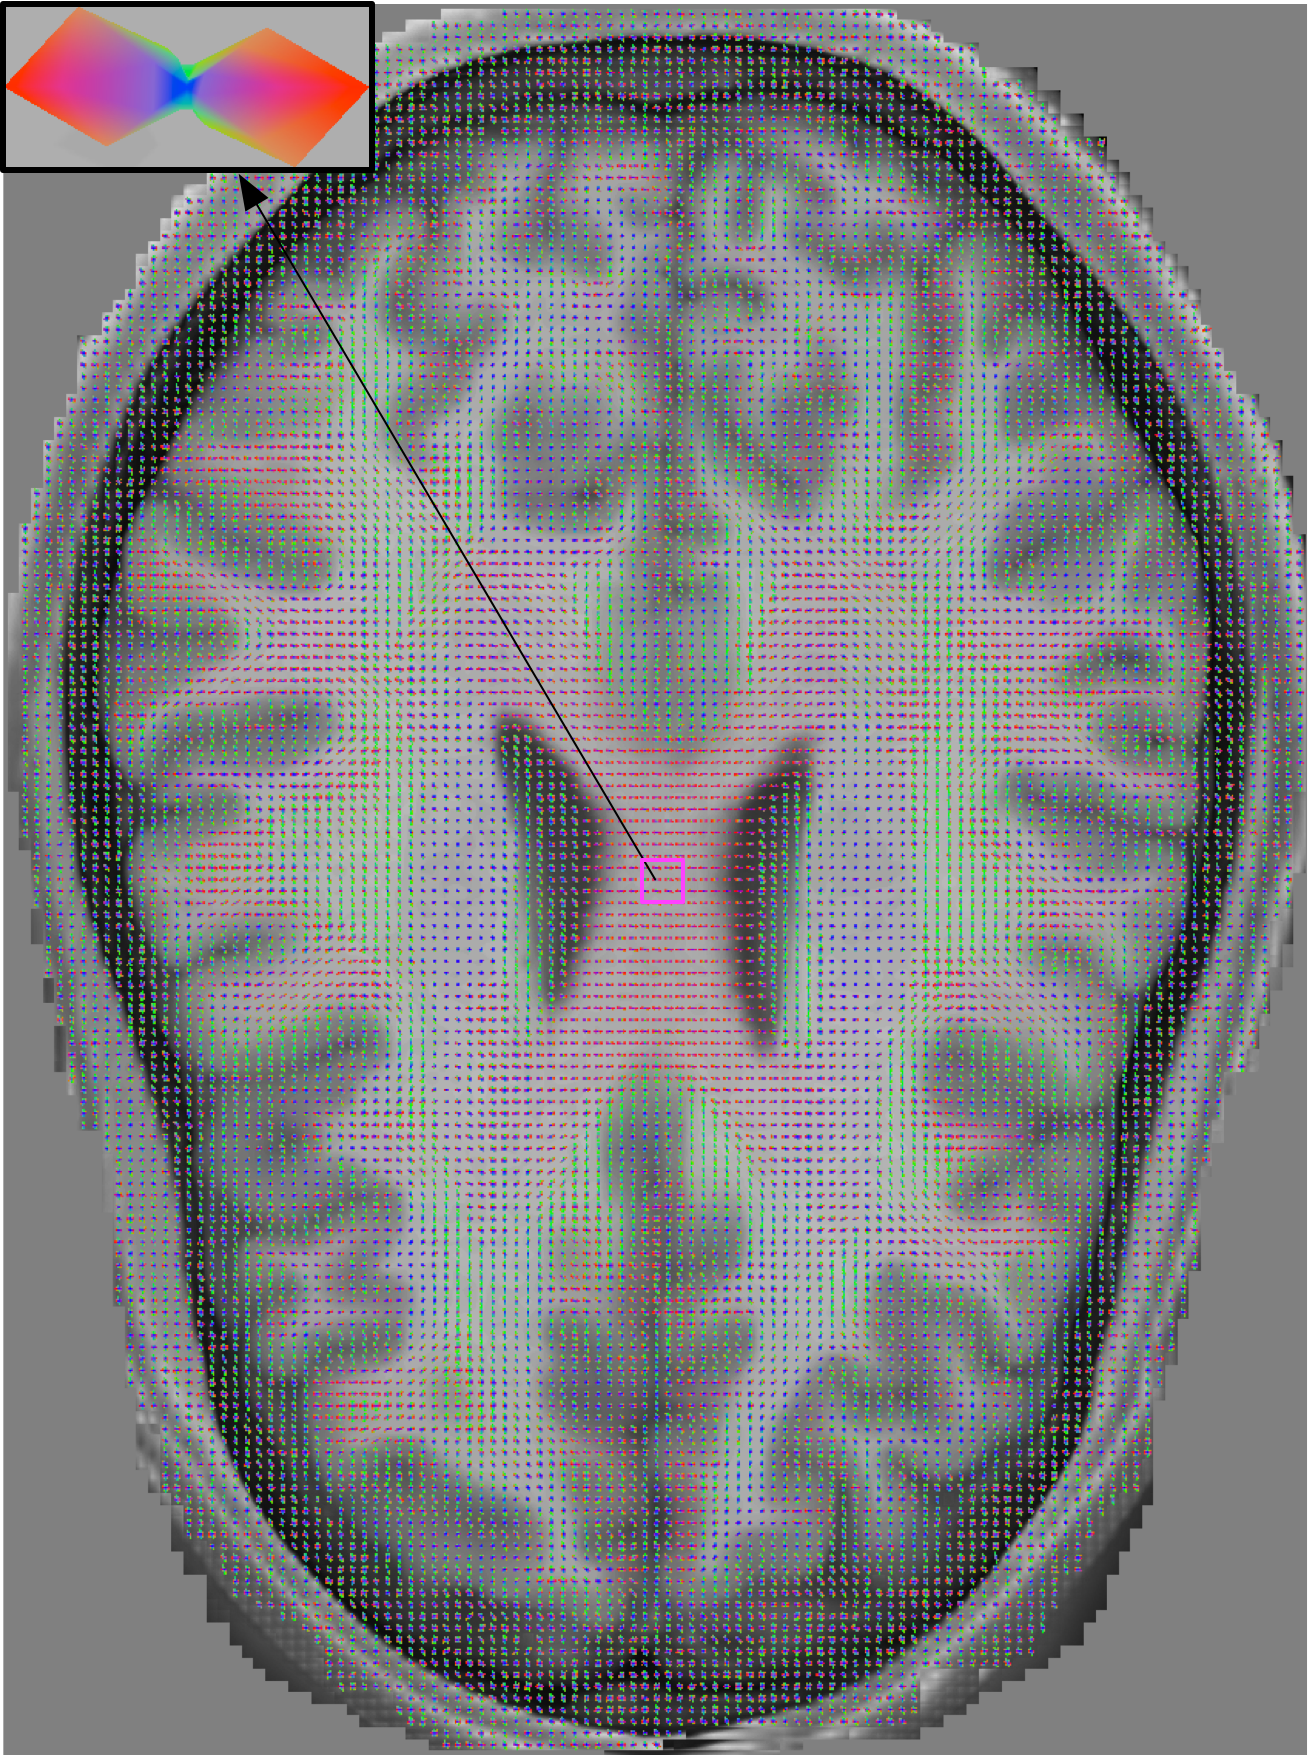
\includegraphics[width=1.0\linewidth, angle=0]{figs/Renderizacao_glifos_evolucao/Adaptividade-multimodal/Fatia_glifo_tf_42_leg.png}
      \caption{13205 glifos renderizados sobre uma fatia axial de um volume de ressonância magnética ponderada em T1. A resolução do glifo corresponde à  tesselação de $2^a$ ordem do icosaedro.}
       \label{fig::qualidade_visual_longe_lowres}
  %   \hspace{1pt}
 \end{figure}
 
  \begin{figure}[H]
 %\subfigcapskip = -5pt
     \centering
     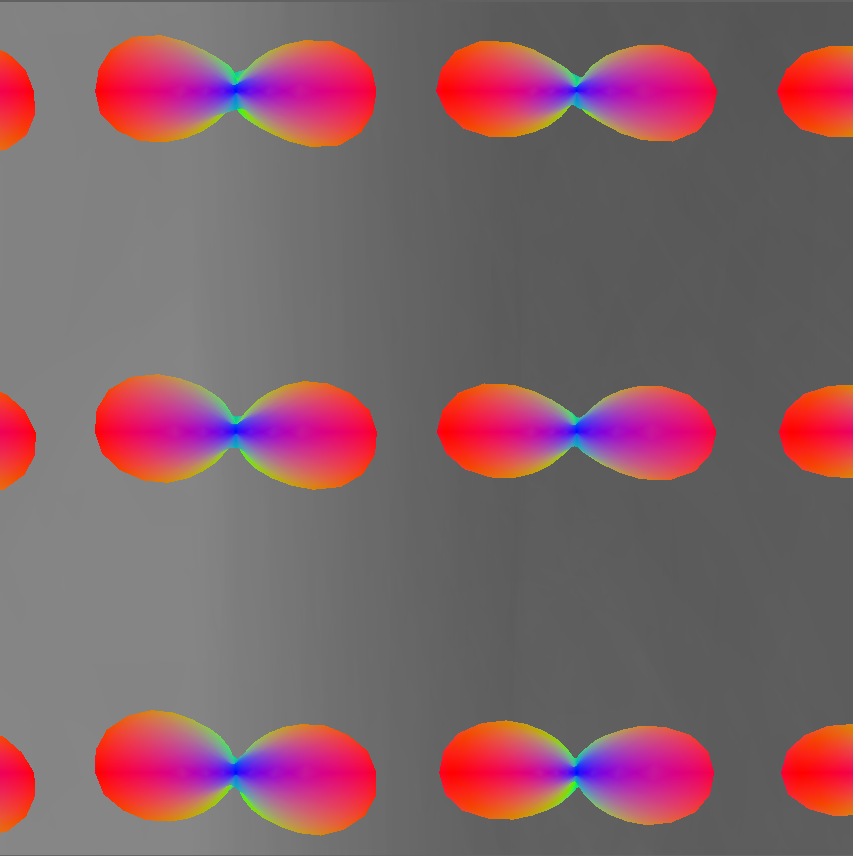
\includegraphics[width=0.5\linewidth, angle=0]{figs/Renderizacao_glifos_evolucao/Adaptividade-multimodal/fatia_perto.png}
      \caption{12 glifos renderizados para 12 \textit{voxels} visíveis (6 renderizados por inteiro), correspondentes à área destacada com o retângulo magenta na fatia axial da Fig. \ref{fig::qualidade_visual_longe_lowres}. Fator de escala de 91,05. Os glifos foram gerados a partir da tesselação de oitava ordem do icosaedro}
       \label{fig::multimodal_glifo_odf_zoom}
  %   \hspace{1pt}
 \end{figure}
 
 
 
% \begin{figure}[H]
% \centering
% %\captionsetup[subfloat]{farskip=0pt,nearskip=0pt}
%     %\rule{6cm}{3cm}
%     \subfloat[centro semioval - axial]{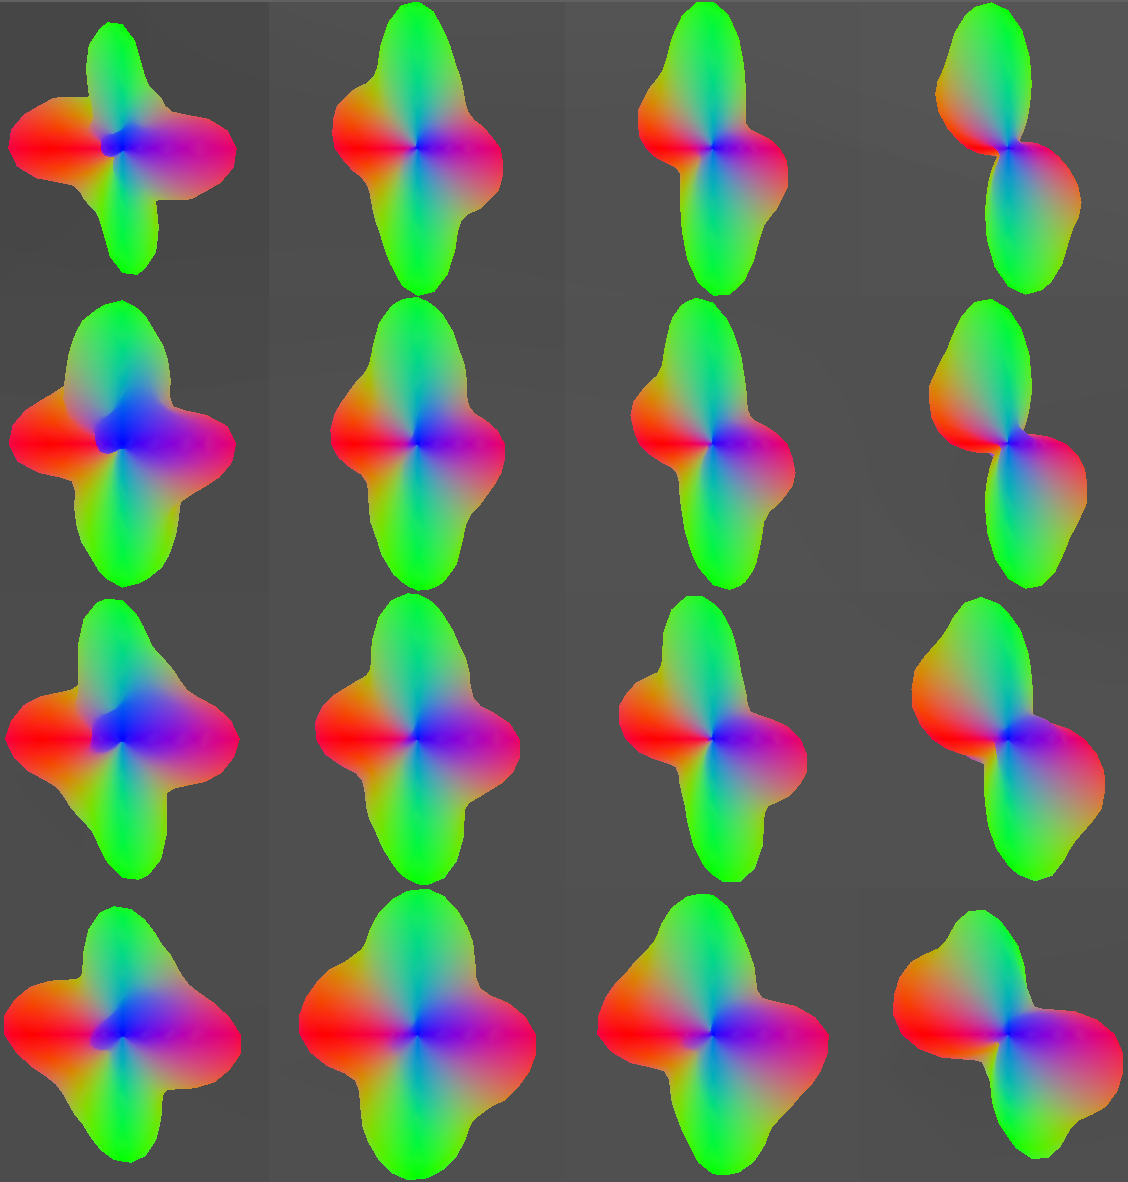
\includegraphics[width=.45\linewidth, angle=0]{figs/Esquema_Glifo/Visual/Glifo_Fatia78_Axial_Top/glifos_16.png}
%     \label{fig::multimodal_glifo_odf_zoom_axial_16}
%     }
%     \subfloat[centro semioval - coronal] {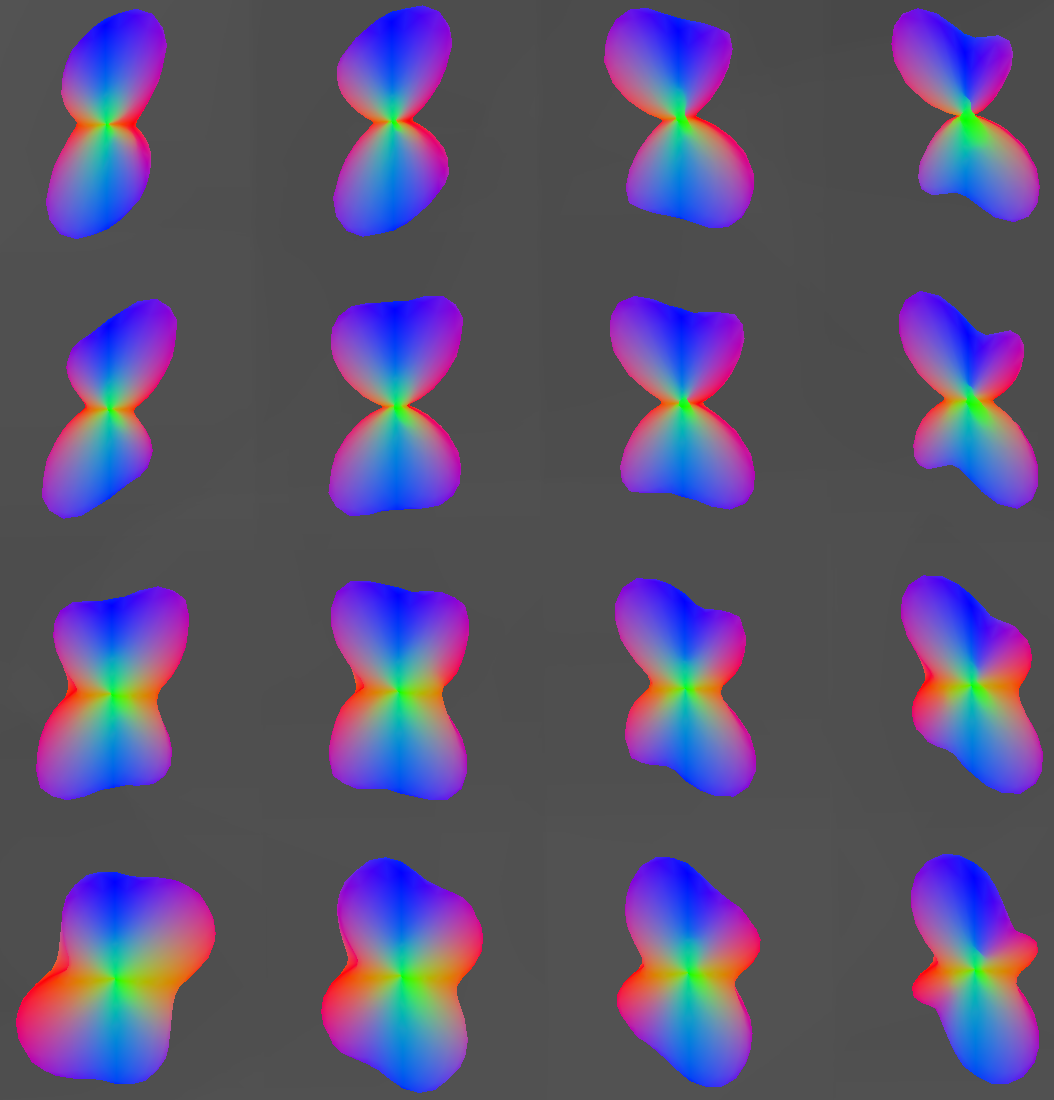
\includegraphics[width=.45\linewidth, angle=0]{figs/Esquema_Glifo/Visual/Glifo_Fatia79_Coronal_front/fatia_16.png}
%     \label{fig::multimodal_glifo_odf_zoom_coronal_16}
%     }
%     \caption{Glifos ODF a um fator de escala de 59,27. A malha é proveniente da $8^a$ ordem de tesselação do icosaedro.}
%     \label{fig::multimodal_glifo_odf_zoom}
% \end{figure}
%%%%%%%%%%%%%%%%%%%%%%%%%%%%%%%%
Para evidenciar similaridades entre as imagens geradas com glifos de resolução maior (da ordem 8$^a$) em relação aos de baixa resolução (da ordem 2$^a$ e ordem 1) em cenas onde a cobertura dos \textit{pixels} por glifo, $max_P$, é muito baixa, apresentamos nas Fig. \ref{fig::qualidade_visual_longe_highres} e \ref{fig::qualidade_visual_longe_lowres_0} imagens da mesma tomada da Fig. \ref{fig::qualidade_visual_longe_lowres}, porém com os glifos de resolução correspondente, respectivamente, à tesselação da ordem 8$^a$ e 1$^a$ (o próprio icosaedro).

%Fig. \ref{fig::multimodal_teste_zoom} ilustra o ambiente de visualização multimodal em uma situação de limiar entre duas resoluções. Nas Fig. \ref{fig::multimodal_162_hollow} e \ref{fig::multimodal_162_filled}, o valor de $max_p$ é de 1368 \textit{pixels}, e em \ref{fig::multimodal_642_hollow} e \ref{fig::multimodal_642_filled}, é de 1444. De acordo com Eq. \ref{eq::icosa_order}, o limiar de mudança de resolução é $max_p = 1406.25$.  Os glifos mostram uma visão axial do corpo caloso, cujo comportamento de difusão ocorre predominantemente na direção esquerda-direita.
%Fig. \ref{fig::multimodal_teste_loc} mostra a localização da região mostrada em Fig. \ref{fig::multimodal_teste_zoom}.
%As Fig. \ref{fig::multimodal_162_hollow} e \ref{fig::multimodal_642_hollow} consistem em apenas o contorno dos triângulos das Fig. \ref{fig::multimodal_162_filled} e \ref{fig::multimodal_642_filled}  para ilustração da mudança de malha.  As imagens foram geradas a partir de uma janela $500 \times 500$ com uma diferença sutil no fator de escala entre ambas.

%\todo[inline]{Não se consegue distinguir os glifos em wireframe dos preenchidos na Fig. \ref{fig::multimodal_teste_zoom}. Como então fazer análises comparativas entre as duas imagens?}

%\begin{figure}[htb]
%\centering
%\captionsetup[subfloat]{farskip=0pt,nearskip=0pt}
%    \subfloat[$4^a$ ordem de tesselação - apenas contornos dos triângulos] {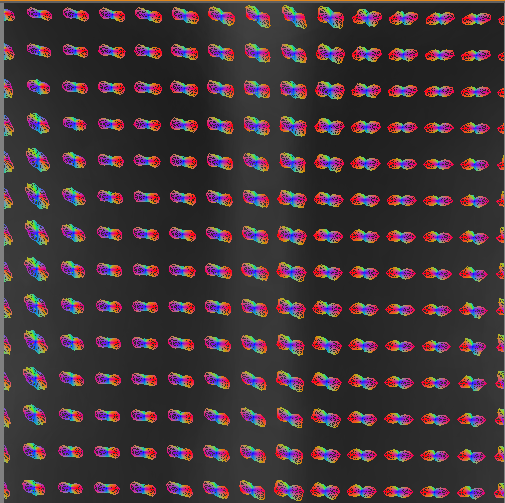
\includegraphics[width=.49\linewidth, angle=0]{figs/Esquema_Glifo/Teste_transicao/162_Hollow.png}
    %\label{fig::multimodal_162_hollow}
%    }
%    \subfloat[$4^a$ ordem de tesselação - triângulos %preenchidos] {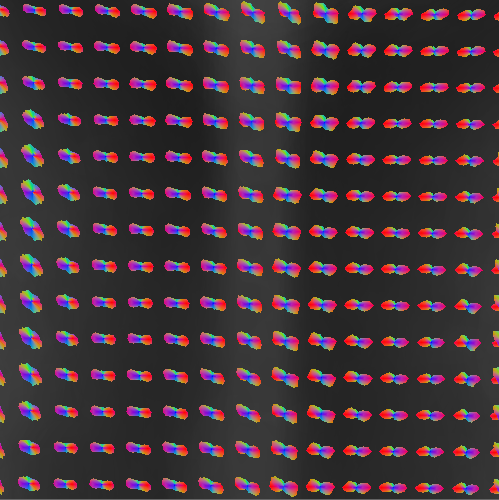
\includegraphics[width=.485\linewidth, %angle=0]{figs/Esquema_Glifo/Teste_transicao/162_filled.png}
%    \label{fig::multimodal_162_filled}
%    }
%    \hspace{1pt}
%    \subfloat[$8^a$ ordem de tesselação - apenas contornos dos triângulos] {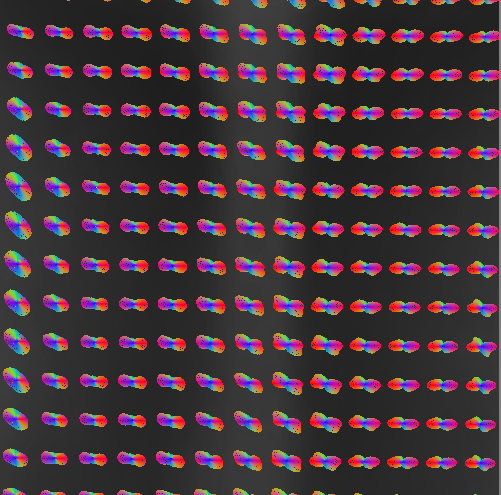
\includegraphics[width=.495\linewidth, angle=0]{figs/Esquema_Glifo/Teste_transicao/642_hollow.png}
%    \label{fig::multimodal_642_hollow}
%    }
%    \subfloat[$8^a$ ordem de tesselação - triângulos preenchidos] {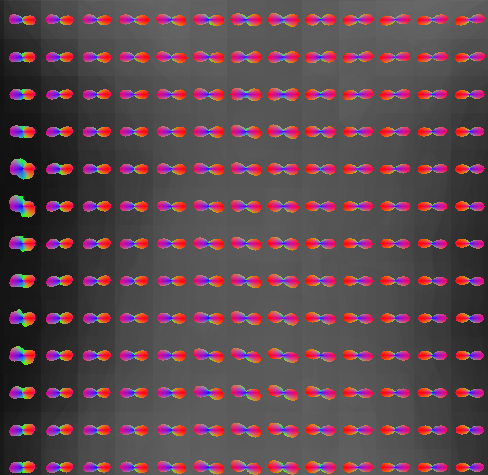
\includegraphics[width=.487\linewidth, angle=0]{figs/Esquema_Glifo/Teste_transicao/642_filled.png}
%    \label{fig::multimodal_642_filled}
%    }
%    \caption{Ilustração da troca de resolução efetuada automaticamente a partir de $max_p$. A troca de resolução ocorre entre as geometrias base derivadas da $4^a$ (\ref{fig::multimodal_162_hollow} e \ref{fig::multimodal_162_filled}) e $8^a$ (\ref{fig::multimodal_642_hollow} e \ref{fig::multimodal_642_filled}) ordem de tesselação.% A região ilustrada é do corpo caloso, próximo a divisa com o ventrículo lateral com  que está em destaque na Fig. \ref{fig::multimodal_teste_loc}.
%    }
%    \label{fig::multimodal_teste_zoom}
%\end{figure}


  \begin{figure}[H]
 %\subfigcapskip = -5pt
     \centering
     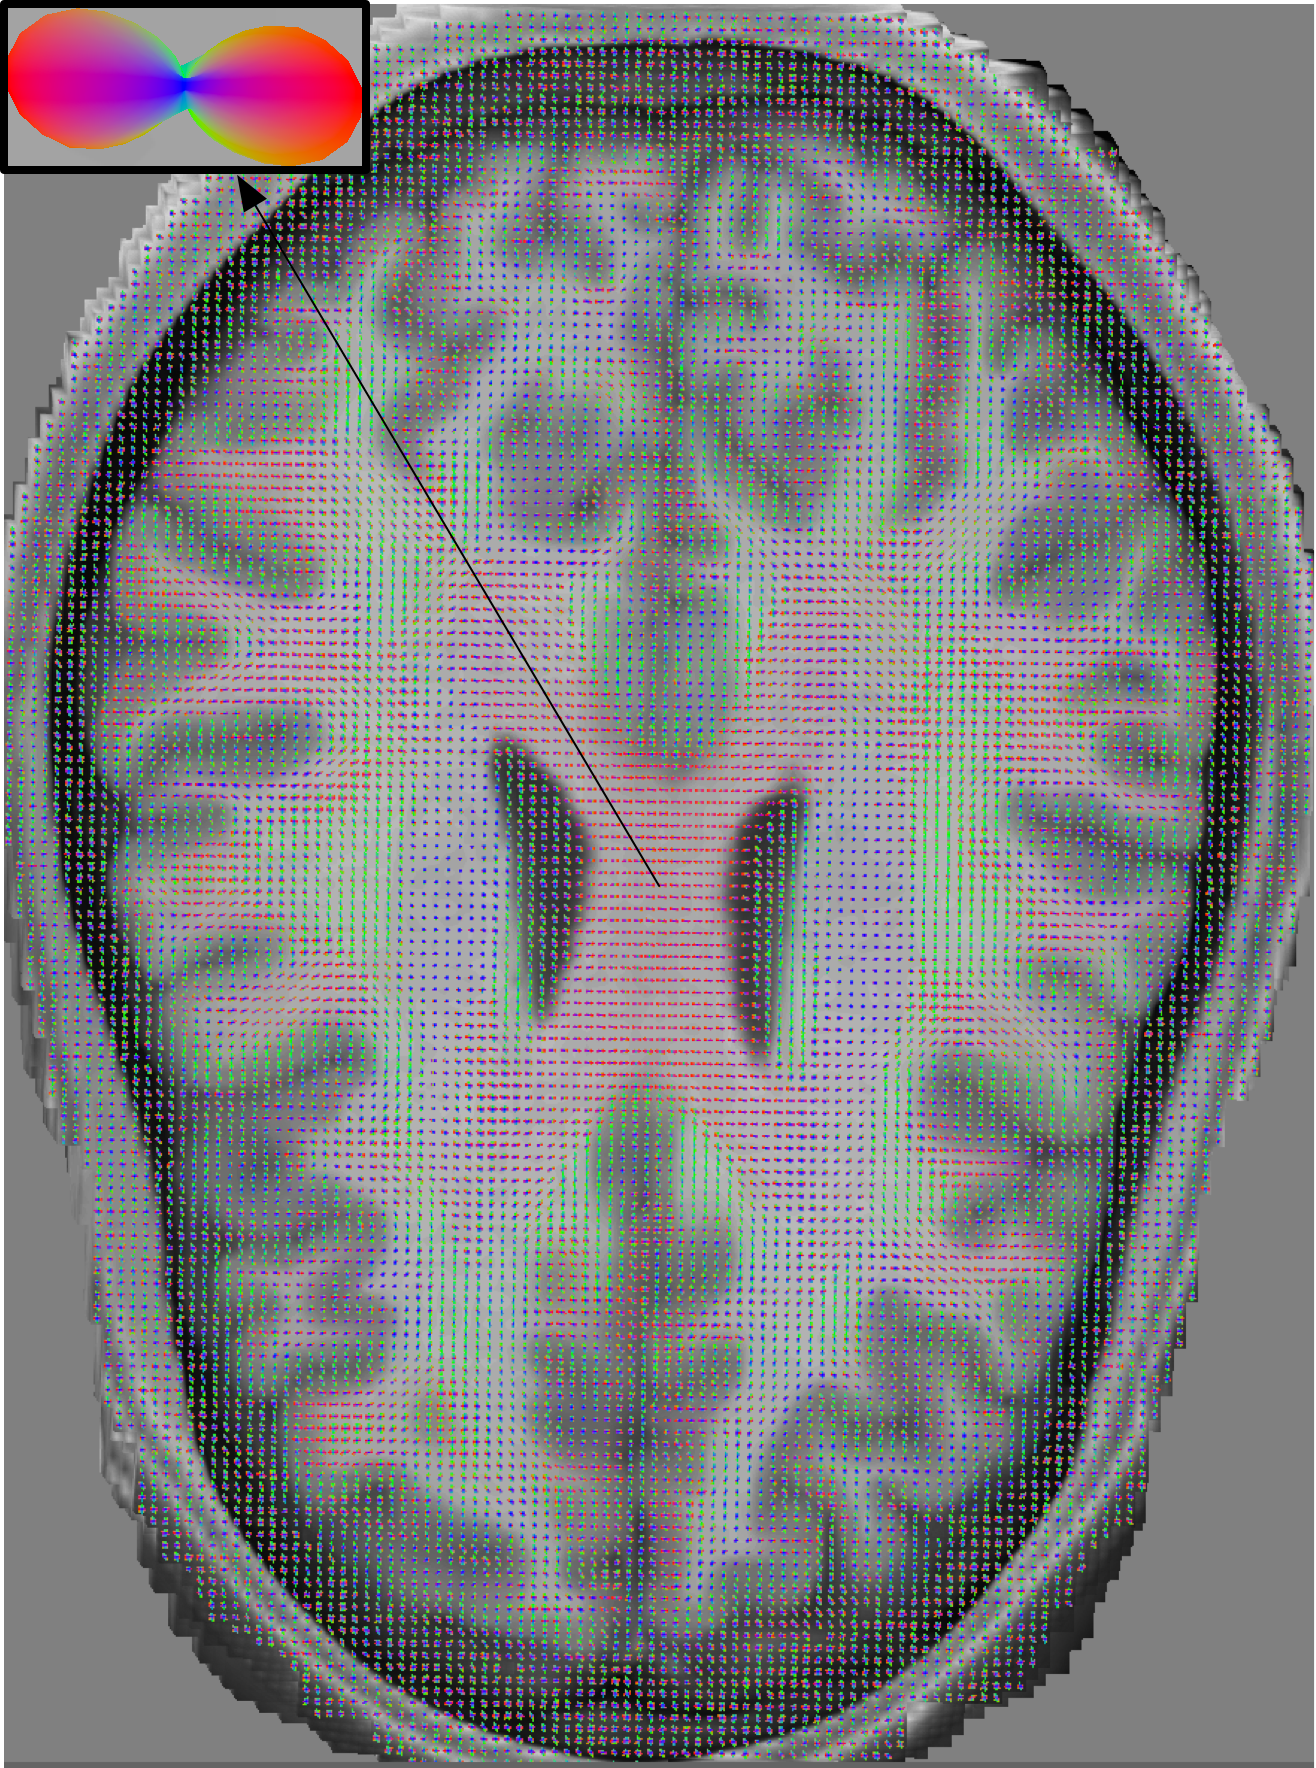
\includegraphics[width=1.0\linewidth, angle=0]{figs/Renderizacao_glifos_evolucao/Adaptividade-multimodal/Fatia_glifo_tf_642.png}
      \caption{13205 glifos renderizados sobre uma fatia axial de volume de ressonância magnética ponderada em T1. Os glifos são gerados a partir da malha esférica obtida pela tesselação de $8^a$ ordem do icosaedro.}
       \label{fig::qualidade_visual_longe_highres}
  %   \hspace{1pt}
 \end{figure}

\begin{figure}[H]
 %\subfigcapskip = -5pt
     \centering
     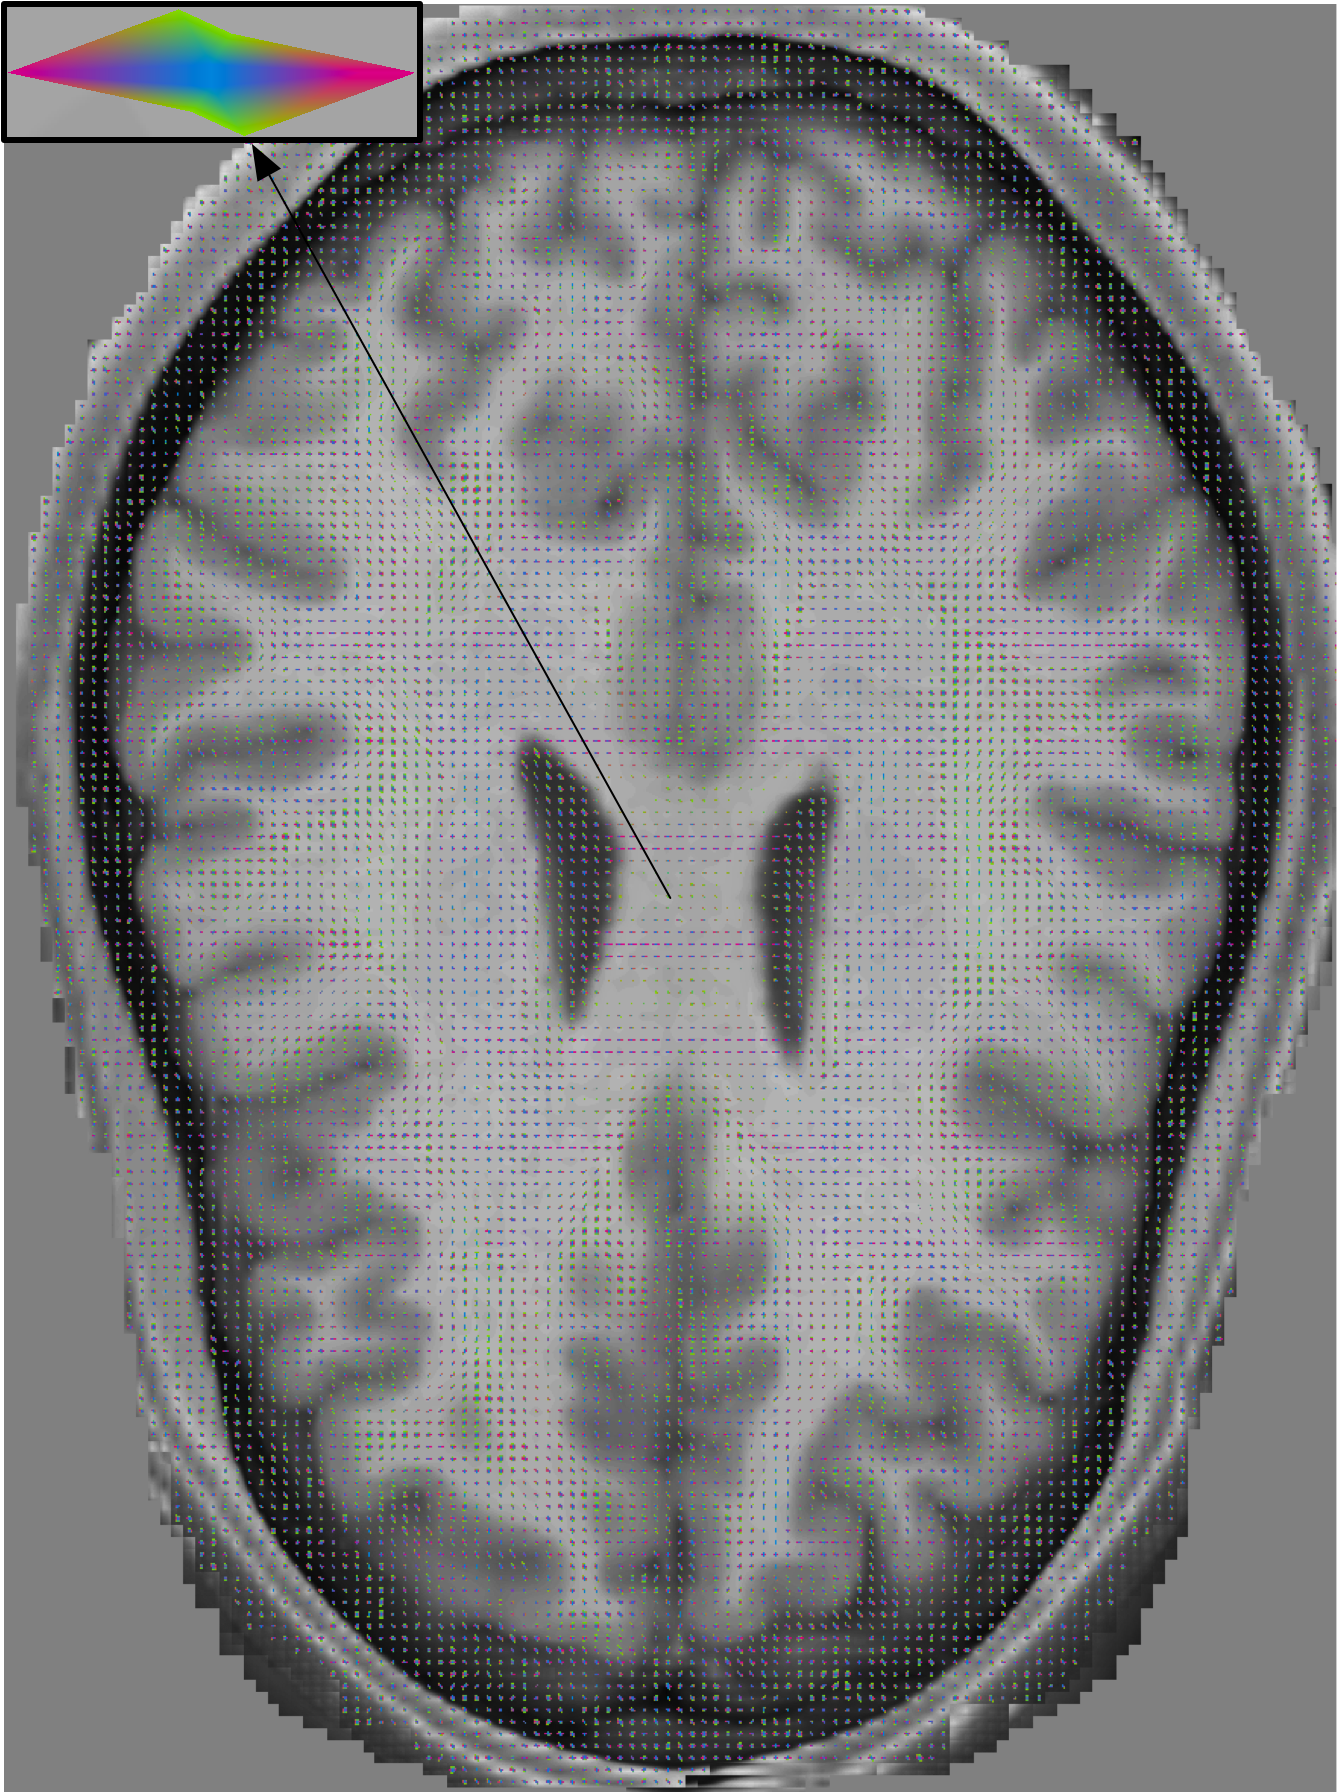
\includegraphics[width=1.0\linewidth, angle=0]{figs/Renderizacao_glifos_evolucao/Adaptividade-multimodal/Fatia_glifo_tf_12.png}
      \caption{13205 glifos renderizados sobre uma fatia axial de um volume de ressonância magnética ponderada em T1. O glifo é gerado a partir do icosaedro (tesselação de $1^a$ ordem).}
       \label{fig::qualidade_visual_longe_lowres_0}
  %   \hspace{1pt}
 \end{figure}


 %\todo[inline]{Sugiro que plote em gráficos os dados abaixo, para manter a uniformidade, e deslocar os dados numéricos para apêndice ... Seria interessante ter os dados numéricos de todos os gráficos no apêndice (por uniformidade). Destacar com linhas trajecadas os fatores de escala em que ocorrem transições de ordens de tesselação. \textcolor{green}{Coloquei as duas tabelas no apêndice. Preparei todos as tabelas de dados e coloquei no apêndice.}}
 
 %\todo[inline]{Legenda da Tabela \ref{tab::glyph_info_experiment_fixed} está estranho ... Você quis dizer que a última linha são parâmetros de renderização da Fig. \ref{fig::qualidade_visual_longe_highres}? \textcolor{green}{Sim. Solucionei explicitando a imagem como um resultado para o experimento}}





%\todo[inline]{Além de não ter selecionado regiões apropriadas (ventrículo lateral !), não é muito clara a visualização dos seus glifos nem RMI-T1 no fundo para as pessoas poderem se contextualizar. Não são nada informativas as Figs. 4.6 e 4.7. Sugiro que faça escolhas melhores. Veja as regiões discutidas em \cite{descoteaux2015}.}

%\todo[inline]{A região que você destacou é ventrículo lateral ... Os glifos deveriam ser isotrópicos pois só há liquido cefalorraquidiano ... Dê uma conferida \textcolor{green}{Verdade! os glifos estão bem na fronteira da corpo caloso para a região.}}
%\begin{figure}[H]
    %\centering
    %\rule{6cm}{3cm}
    %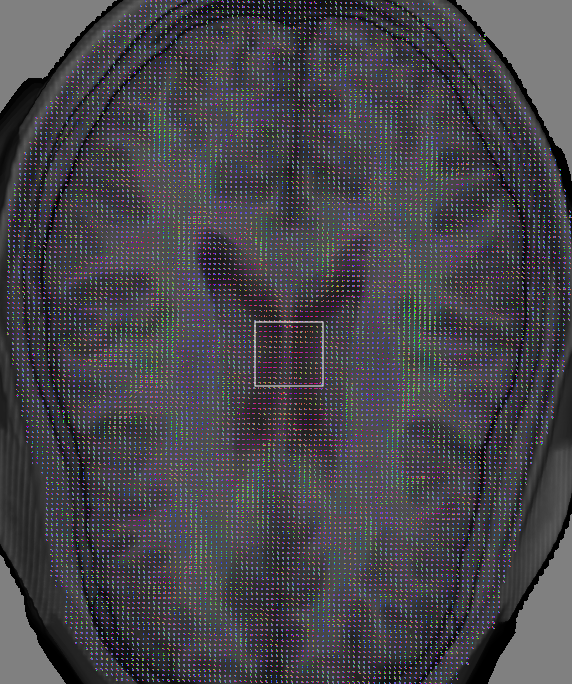
\includegraphics[width=.56\linewidth, angle=0]{figs/Esquema_Glifo/Teste_transicao/base_teste_zoom.png}
    %\caption{MRI T1 anatômico co-registrado com DWI. A região dentro do contorno quadrado branco corresponde a região analisada na Fig. \ref{fig::multimodal_teste_zoom}.}
    %\label{fig::multimodal_teste_loc}
%\end{figure}

\subsection{Discussões}

%\todo[inline]{Revisar bem o texto. Está totalmente desconexo. \textcolor{green}{OK!}}

Observe na Fig. \ref{fig::fps_fatorescala} que, para fatores de escala menores que 10, a quantidade de glifos pode chegar a 13205 glifos, e o desempenho do algoritmo na renderização dos glifos com a resolução correspondente à tesselação da ordem 8$^a$ do icosaedro (linha azul) cai drasticamente. A redução da resolução para 2$^a$ (linha magenta) e 4$^a$ ordens (linha preta) permite que o tempo de resposta do sistema se mantenha interativo.

O gráfico na Fig. \ref{fig::fps_fatorescala} e a Tabela \ref{tab::glyph_info_experiment} no apêndice mostram que, em um fator de escala menor que 10 e muitos glifos sendo renderizados, há uma queda abrupta no desempenho, em FPS, da renderização dos glifos de resolução correspondente à tesselação de 8$^a$ ordem do icosaedro (linha azul). Ao compará-la com a estratégia de multi-resolução (linha multi-cores), temos um ganho em aproximadamente 8,63 FPS quando 13205 glifos (fator de escala = 1,59) são renderizados (linha magenta) e em 6,3 FPS quando pouco mais de 9166 glifos (fator de escala = 2,4) são renderizados.

Por outro lado, o tempo de resposta da abordagem multi-resolução se torna menor que a abordagem de resolução fixa para um fator de escala acima de 10, porém ambos estão sendo renderizados a taxas interativas na faixa de 30 FPS \cite{nielsen1994} e o usuário tem a sensação que o sistema reage de forma instantânea a sua interação. As perdas em desempenho para visualização sem multi-resolução para fatores de escala menores que 10, em que a taxa de quadros do ambiente de visualização se torna menor que 10 FPS, faz com que a configuração multi-resolução seja uma adição agregadora ao algoritmo proposto.%Isto não ocorre na visualização sem multi-resolução com fator de escala menor do que 10, na qual a taxa de quadros do sistema é menor que 10 FPS, e o usuário percebe o atraso de resposta, o que não ocorre com a configuração de multi-resolução.

Fazendo uma análise visual das Fig. \ref{fig::qualidade_visual_longe_lowres},  \ref{fig::qualidade_visual_longe_highres} e \ref{fig::qualidade_visual_longe_lowres_0}, nas quais 13205 glifos são renderizados a um fator de escala igual a 1,59 e $max_p = 36$ (Tabela \ref{tab::glyph_info_experiment}), certificamos que, para um fator de escala baixo, as diferenças entre as formas dos glifos gerados a partir das tesselações de segunda e oitava ordens do icosaedro, e até de primeira ordem para fatores de escala mais baixos, são imperceptíveis visualmente. Num nível de fator de escala próximo de 1, a informação que os glifos carregam para o usuário se deve mais às cores do que às suas formas. Mesmo que essa diferença não seja distinguível quando $max_p$ seja em algumas unidades de \textit{pixels}, optamos por excluir a primeira ordem na abordagem multi-resolução (Eq. \ref{eq::icosa_order}).

%Fazendo uma análise visual das Fig. \ref{fig::qualidade_visual_longe_lowres},  \ref{fig::qualidade_visual_longe_highres} e \ref{fig::qualidade_visual_longe_lowres_0}, nas quais 13205 glifos são renderizados a um fator de escala igual a 1,59 e $max_p = 36$ (Tabela \ref{tab::glyph_info_experiment}), certificamos que, para um fator de escala baixo, as diferenças entre as formas dos glifos gerados a partir das tesselações de segunda e oitava ordens do icosaedro, são imperceptíveis visualmente, enquanto não é possivel inferir sobre os glifos posicionados nos \textit{voxels} na primeira ordem de tesselação. Num nível de fator de escala próximo de 1, a informação que os glifos carregam para o usuário se deve mais às cores do que às suas formas. Para fatores de escala menores, mesmo que a diferença não seja distinguível quando $max_p$ esteja na faixa de algumas unidades de \textit{pixels}, optamos mesmo assim por não utilizar a primeira ordem na abordagem multi-resolução (Eq. \ref{eq::icosa_order}).

%\sout{Fazendo uma análise visual em Fig. \ref{fig::multimodal_teste_zoom}, em que a imagem renderizada tem um $max_p$ próximo da transição de resolução entre a quarta e oitava ordem de tesselação para os glifos, pode-se perceber que o aumento e diminuição de resolução ocorrem de forma sutil, sendo somente perceptível quando os triângulos não são preenchidos (Fig. \ref{fig::multimodal_162_hollow} e \ref{fig::multimodal_642_hollow}), o que torna o modelo que utilizamos para fazer as transições de resolução adequado neste contexto.}

Caso o usuário queira analisar os glifos mais de perto ou aumentar o tamanho da janela, fazendo-a cobrir mais \textit{pixels}, o glifo é gerado a partir de uma malha suave o suficiente para que ele possa visualizar os detalhes do comportamento das dODFs. Caso o usuário queira ter uma visão mais geral do volume com os glifos e diminuir o fator de escala, diminuímos a resolução de cada glifo renderizado para aliviar o processamento computacional associado a cada um deles. %\sout{Os glifos destacados nos cantos das Figs. \ref{fig::qualidade_visual_longe_lowres},  \ref{fig::qualidade_visual_longe_highres} e \ref{fig::qualidade_visual_longe_lowres_0} ilustram as geometrias dos glifos renderizados.}

%\todo[inline]{O parágrafo abaixo contraria a sua proposta em que você monta os dados de ODF de forma hierarquizada. Quando a maior ordem é 16, os dados de outras ordens são subconjuntos! Há alguma incoerência na sua afirmação!}
%\sout{Em contrapartida, Mesmo com os ganhos documentados em FPS da multi-resolução, há uma considerável diminuição em FPS para fatores de escala de 1,5 e 2,4, nos quais tem 13205 e 9032 glifos renderizados. O gargalo que diminui o desempenho do algoritmo está relacionado ao alto tráfego de dados GPU-CPU com as coordenadas dos \textit{voxels} detectados. Nesta abordagem de renderização, não podemos compensar este gargalo pois a alta dimensionalidade das ODFs torna inviável o seu armazenamento completo na GPU, como tem sido uma das soluções de \citeonline{voltoline2021} para renderizar superquádricos com alta escalabilidade em tempo interativo.}

Com esta série de experimentos, mesmo com a diminuição do FPS para muitos glifos ODF renderizados, podemos concluir através dos testes feitos que o algoritmo de renderização proposto integrado ao ambiente de visualização multimodal gera imagens com glifos ODF em taxas interativas na máquina utilizada para testes, dentro dos limites estabelecidos por \citeonline{nielsen1994}.

%%%%%%%%%%%%%%%%%%%%%%%%%%%%%%%%%%%%%%%%%%%%%%%%%%%%%%%%%%%%%%
\section{Aspectos visuais e interpretabilidade}
%\section{Glifos ODF integrados ao ambiente de visualização multimodal}
\label{sec::aspectos_visuais_e_interpretabilidade}

%\todo[inline]{Quando sugeri este experimento, pensei mais na avaliação comparativa entre os glifos existentes para DWIs e discutir onde se inserem os seus resultados. A ideia de gerar tratos nas regiões em que você vai mostrar os seus glifos é para o leitor possa entender os resultados esperados e avaliar por ele mesmo se o que ele vê nos seus glifos corresponda à realidade.}

%\sout{Propomos um experimento para avaliar aspectos visuais do nosso algoritmo de esquema de renderização em comparação às superquádricos. Para isso, exibiremos regiões onde diferentes tratos coexistem nos mesmos \textit{voxels} e as comparamos com os glifos superquádricos \cite{Kindlmann2004} do DTI, que também estão integrados ao ambiente de visualização.}

Embora seja conhecida na literatura a superioridade dos glifos ODF em relação aos grifos superquádricos quanto ao poder informativo em difusões múltiplas intravóxeis, apresentamos nesta seção um grupo de experimentos que nos permita avaliar a nossa implementação de glifos ODF em relação aos glifos superquádricos, cuja renderização multimodal foi proposta por \citeonline{voltoline2021}, em regiões de múltiplas direções de difusão. As regiões consistem no centro semioval (Fig. \ref{fig::relacoes_espaciais_feixes}), onde ocorre o cruzamento do trato\footnote{Tratos são conjuntos de fibras organizadas em feixe que conectam diferentes partes do cérebro e geralmente são nomeados de acordo com sua origem e terminação.} cortico-espinhal (CS), corpo caloso (CC), fascículo longitudinal superior (\textit{superior longitudinal fasciculus}, SLF), na interface entre corpo caloso e cíngulo, onde há o ``beijo'' (\textit{kissing}) das fibras do corpo caloso na região medial com o cíngulo, e na coroa radiada, nos quais as fibras de corpo caloso e do trato CS se abrem como ``leque'' (\textit{fanning}).

%fibras dos tratos

%https://www.researchgate.net/figure/Brain-circuitry-associated-with-ADHD-https-doiorg-101371-journalpone0175433g003_fig3_316092557

%\todo[inline]{Fig.\ref{fig::relacoes_espaciais_feixes} precisa ser refeita. Sugiro que sejam esboçadas as principais fibras em cortes sagital e coronal como nas ilustrações ...só de forma mais coordenada e com as fibras que vamos trabalhar}
%\begin{figure}[H]
%    \subfloat[Centro semioval] {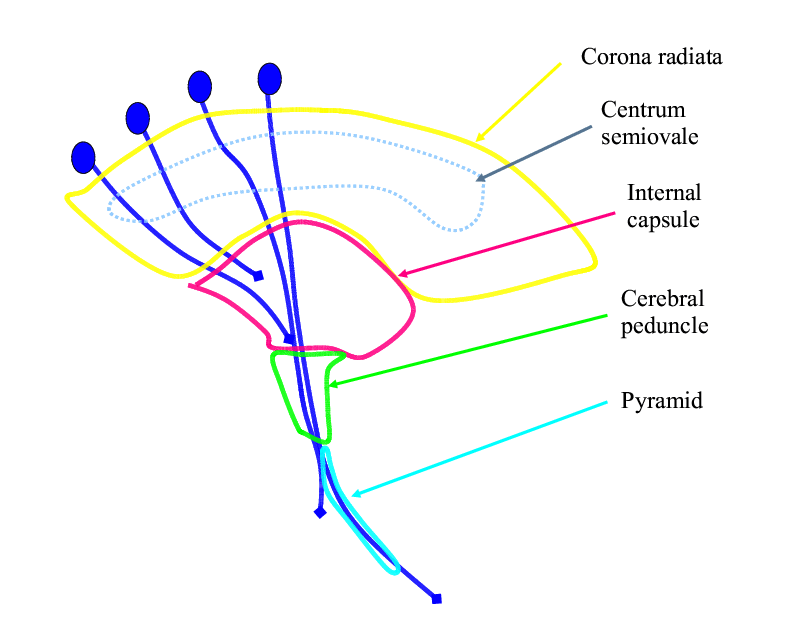
\includegraphics[width=.45\linewidth, angle=0]{figs/esquema_corona_radiata_centrum_semiovale.png}
%    \label{fig::corona_radiata_centrum_semiovale}
%    }
%    \subfloat[Coroa radiata] {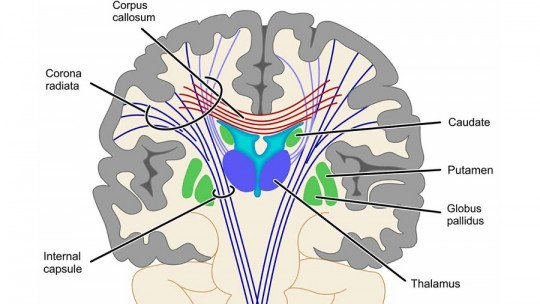
\includegraphics[width=.45\linewidth, angle=0]{figs/capsula-interna-corona-radiata.jpg}
%    \label{fig::esquema_corona_radiata}
%    }
%    \caption{Relações espaciais dos feixes cerebrais.}
%    \label{fig::relacoes_espaciais_feixes}
  %   \hspace{1pt}
% \end{figure}
 
% \begin{figure}[H]
%    % \subfloat[Centro semioval] {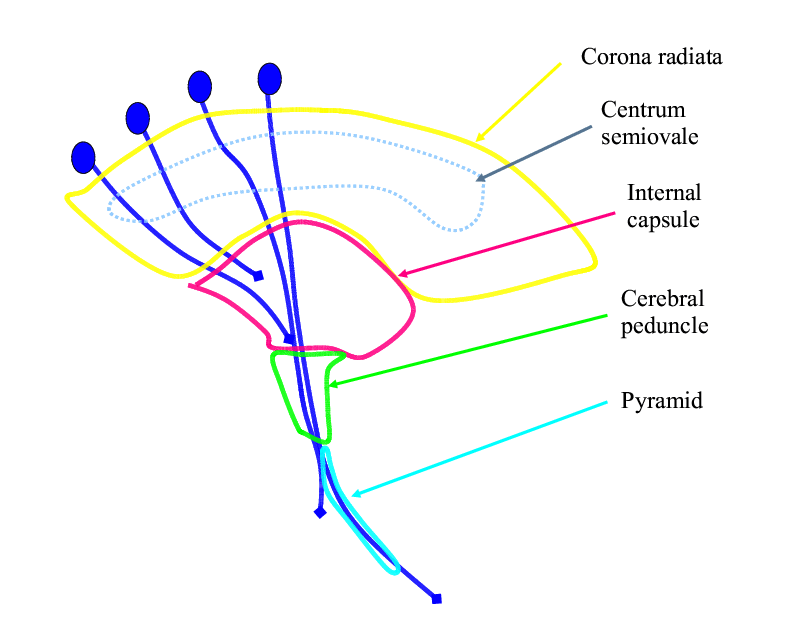
\includegraphics[width=.45\linewidth, angle=0]{figs/esquema_corona_radiata_centrum_semiovale.png}
    % \label{fig::corona_radiata_centrum_semiovale}
    % }
%    \subfloat[Ilustração do Centro Semioval - Fatia coronal ] {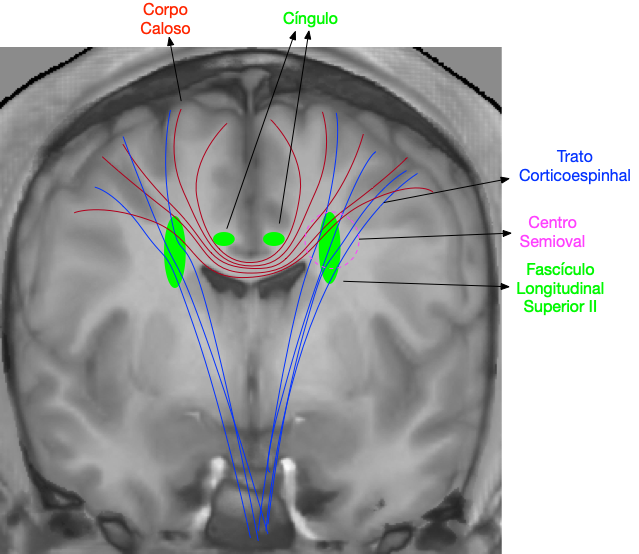
\includegraphics[width=.65\linewidth, angle=0]{figs/ilustracao_centro_semioval.png}
%    \label{fig::esquema_corona_radiata}
%    }
%    \caption{Relações espaciais dos feixes cerebrais analisados no terceiro grupo de experimentos.}
%    \label{fig::relacoes_espaciais_feixes}
  %   \hspace{1pt}
% \end{figure}
 
 \begin{figure}[H]
    % \subfloat[Centro semioval] {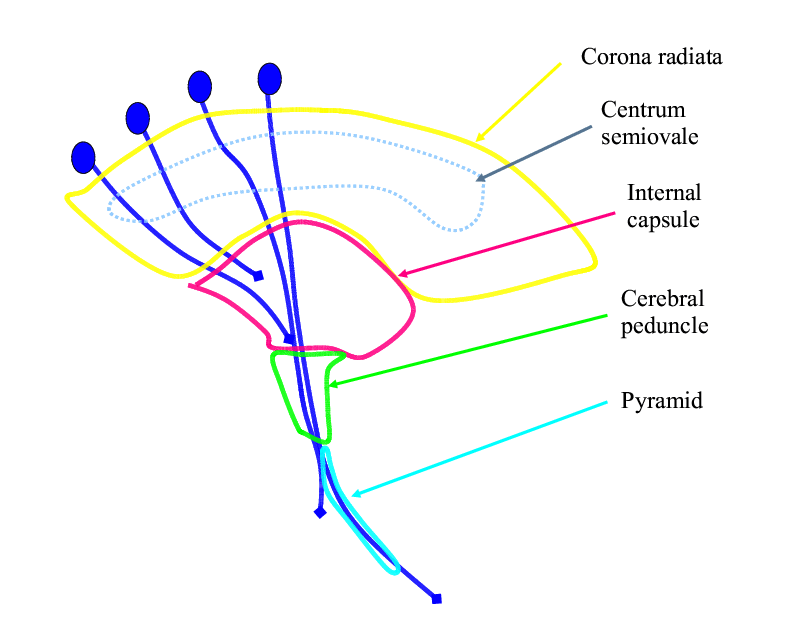
\includegraphics[width=.45\linewidth, angle=0]{figs/esquema_corona_radiata_centrum_semiovale.png}
    % \label{fig::corona_radiata_centrum_semiovale}
    % }
 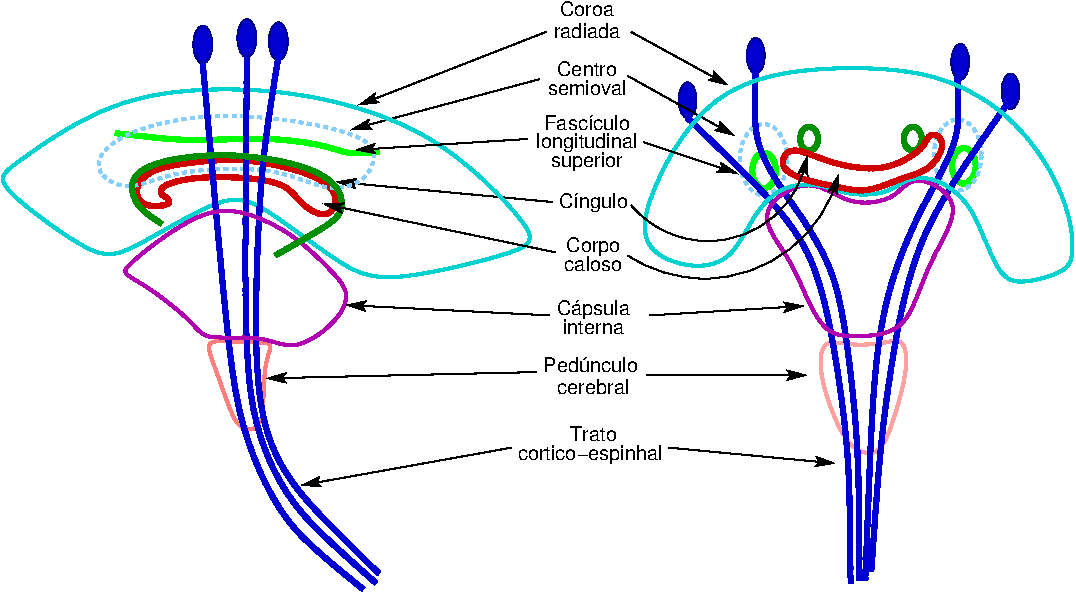
\includegraphics[width=.9\linewidth, angle=0]{figs/esboco_feixes_antomicos.png}
    \label{fig::esquema_corona_radiata}
    
    \caption{Relações espaciais dos feixes cerebrais analisados no terceiro grupo de experimentos.}
    \label{fig::relacoes_espaciais_feixes}
  %   \hspace{1pt}
 \end{figure}

%As difusões intravóxeis no centro semioval são comumente utilizadas para análises qualitativas de métodos de alta ordem.
%\citeonline{tournier2007} e \citeonline{yeh2010} utilizaram  uma fatia axial  para ilustrar resultados do método \textit{constrained spherical deconvolution} e GQI na síntese de direções de difusão intravoxel no centro semioval. Fig. \ref{fig::multimodal_glifo_odf_1} revela duas direções dominantes paralelas ao plano da imagem, uma corresponde à direção das fibra do corpo caloso (vermelho) e a outra à do fascículo longitudinal superior (verde), e a terceira perpendicular ao plano da imagem, correspondente à direção da coroa radiada (azul). Por meio de uma fatia coronal \cite{yeh2010} pode-se ver que as direções do corpo caloso e da coroa radiada são paralelas ao plano da imagem e que a direção do SLF e do cíngulo é perpendicular ao plano, como ilustra a Fig. \ref{fig::multimodal_glifo_odf_1}.

\subsection{Descrição}

Para avaliar a eficácia dos glifos no discernimento das configurações de múltiplas direções de fibras dentro de um \textit{voxel}, procuramos visualizar as funções dODFs em três regiões (Fig. \ref{fig::relacoes_espaciais_feixes}): (1) a interface em forma de ``beijo'' entre corpo caloso e cíngulo, (2) a base em forma de leque da coroa radiada, que conecta a cápsula interna com as áreas corticais,  e (3) o centro semioval, onde se encontram as fibras de associação (SLF), fibras de projeção (coroa radiada) e fibras comissurais (corpo caloso)\footnote{As fibras de associação são axônios que conectam áreas corticais dentro do mesmo hemisfério cerebral. As fibras de projeção são axônios que ligam o córtex cerebral a centros subcorticais. As fibras comissurais são axônios que conectam áreas corticais idênticas dois dois hemisférios cerebrais.}. 

Acima do trecho na parte medial do cérebro do corpo caloso, encontra-se o cíngulo (CG), um feixe de fibras em forma de ``C'' que conecta o giro anterior temporal ao córtex orbitofrontal \cite{fortin2012}. O cíngulo faz parte do sistema límbico e está envolvido com as funcionalidades de atenção, memória e emoções \cite{catani2008}.

A coroa radiada consiste em um conjunto de fibras que tem direção predominantemente ascendente, conectando o tálamo com o córtex cerebral, e é responsável pelas funções motoras, perceptivas e outras funções cognitivas \cite{catani2008}. Pela coroa radiada passam o trato cortico-espinhal e as fibras do corpo caloso. O trato cortico-espinhal (CS) é um conjunto de axônios motores que ligam o córtex motor primário no cérebro (giros pré e pós-central) com a medula espinhal \cite{DTI_Handbook}. O corpo caloso (CC) consiste em fibras que se originam no córtex, convergem até a parte medial do cérebro e seguem em direção ao hemisfério oposto e conecta ambos \cite{fortin2012}. Está envolvido em muitas funções motoras, perceptivas e cognitivas \cite{catani2008}. 



O centro semioval é a região em que o CS, CC e SLF cruzam. O SLF  tem direção predominantemente anteroposterior e é subdividido em cinco componentes: SLF I, SLF II, SLF III, SLF temporoparietal e fascículo arqueado \cite{kamali2014}. A localização dos tratos SLF I, II e III são ilustradas em Fig. \ref{fig::tratos_4}. O par de fibras mais próximo da fissura longitudinal é o SLF I, enquanto os pares mais externos, tanto no hemisfério direito quanto no esquerdo são SLF II e III. O SLF II cruza com o CC e o CS no centro semioval em ambos os hemisférios. Há evidências de que o trato tem um papel na linguagem e controle motor \cite{fortin2012}.%tr \textcolor{red}{Cruza com o corpo caloso e a coroa radiada, o}.  O ponto de cruzamento é denominado centro semioval. A topografia das fibras do cérebro da região a ser analisada pode ser encontrada em \cite{yagmurlu2015}.

Fig. \ref{fig::tratos} ilustra as fibras do CS, CG, CC e SLF que reconstruímos a partir de tensores de difusão (DTI) com uso do VMTK-Neuro \cite{VMTKNeuro}. Mencionamos que, por termos aplicado a técnica DTI, os feixes de fibras mostrados não refletem garantidamente as conexões cerebrais reais como revelam diversos estudos \cite{berman2009, tournier2011, bucci2013, descoteaux2015, SCHILLING2019194}. Porém, tais reconstruções foram fundamentais para nos nortear na identificação das potenciais regiões com múltiplas direções de difusão intravóxel.

%{\includegraphics[width=.4\linewidth, angle=0]

\begin{figure}[H]
\centering
%\captionsetup[subfloat]{farskip=0pt,nearskip=0pt}
    %\rule{6cm}{3cm}
    \subfloat[Visão axial do trato cortico-espinhal.]{\makebox[1.0\width]{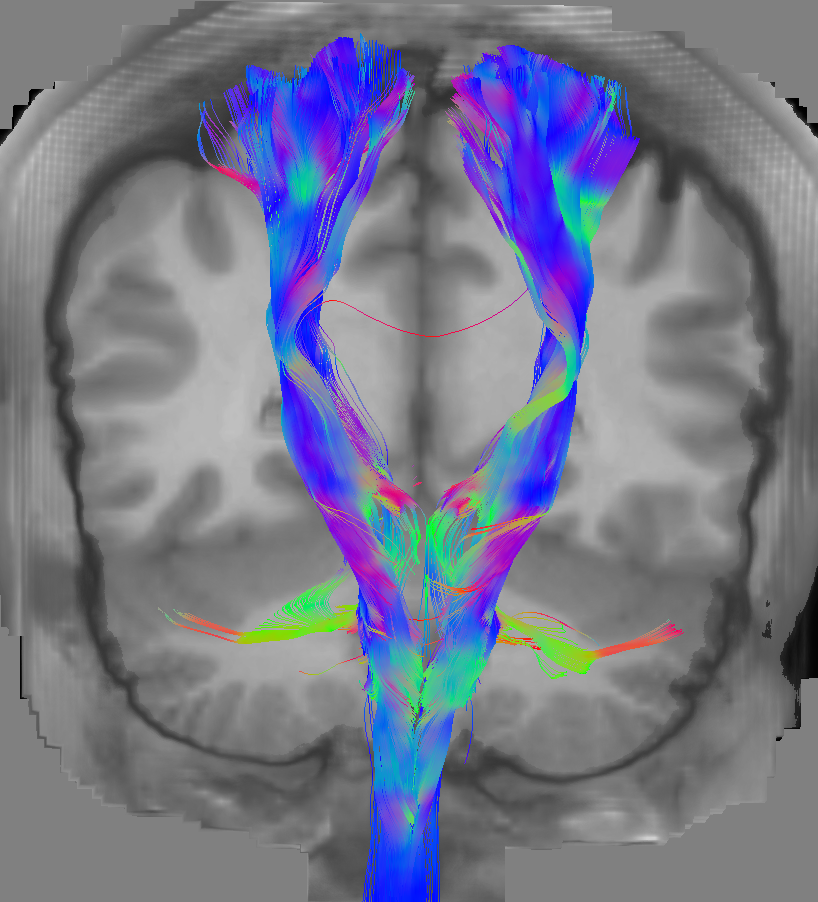
\includegraphics[width=.35\linewidth, angle=0]{figs/Renderizacao_glifos_evolucao/Tratos/trato_1_tf.png}
    }
   \label{fig::tratos_1}
   }
    \subfloat[Visão sagital do cíngulo (fibras curvas).] {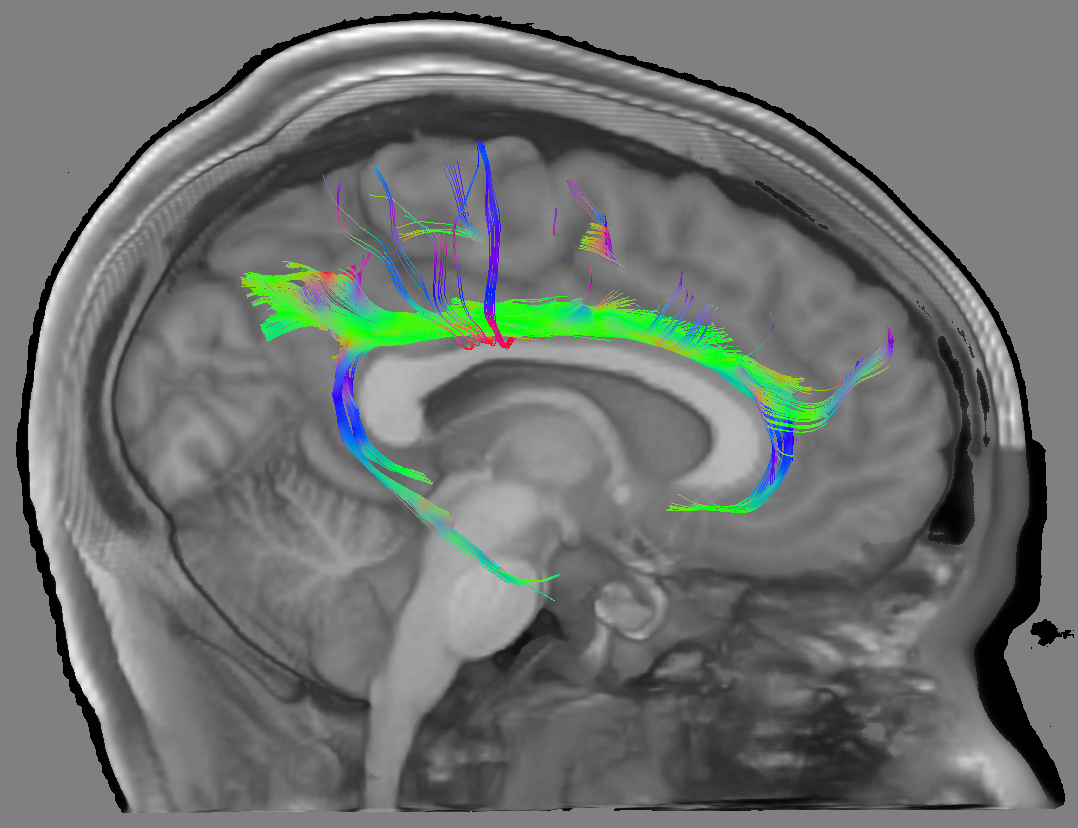
\includegraphics[width=.5\linewidth, angle=0]{figs/Renderizacao_glifos_evolucao/Tratos/trato_3_tf.png}
    \label{fig::tratos_3}
    }
    \\
    \subfloat[Visão axial do corpo caloso.]{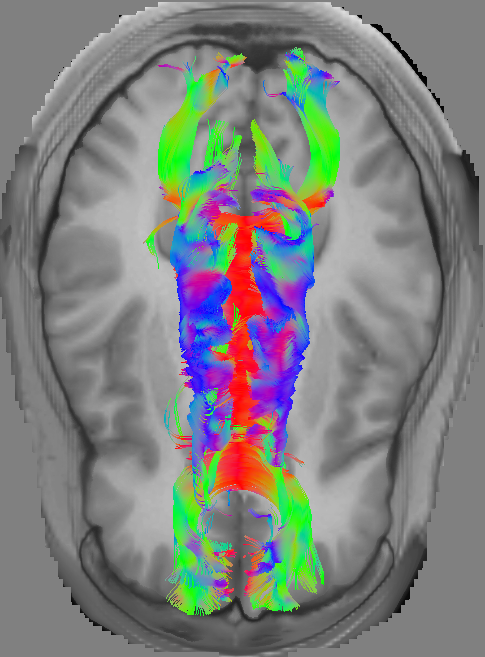
\includegraphics[width=.4\linewidth, angle=0]{figs/Renderizacao_glifos_evolucao/Tratos/trato_2_tf.png}
    \label{fig::tratos_2}
    }
    \subfloat[Visão axial do fascículo Longitudinal Superior.] {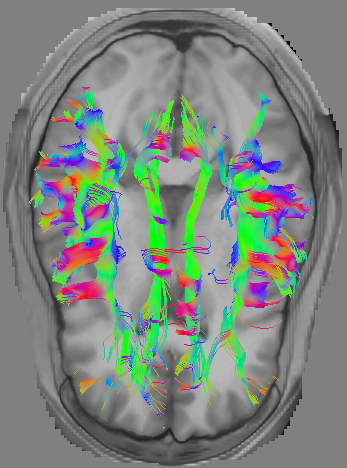
\includegraphics[width=.4\linewidth, angle=0]{figs/Renderizacao_glifos_evolucao/Tratos/trato_4_tf_2.png}
    \label{fig::tratos_4}
    }
    \caption{Feixes de fibras reconstruídos a partir de DTI em VMTK-Neuro \cite{VMTKNeuro}.}
    \label{fig::tratos}
\end{figure}



%Também ilustramos a ........

Sendo o objetivo uma análise visual comparativa entre os glifos superquádricos \cite{Kindlmann2004} e os glifos ODF, geramos ambos os glifos com o mesmo volume utilizado no segundo grupo de experimentos e no mesmo ambiente de visualização multimodal.
Explorarmos os volumes de glifos renderizados sob a perspectiva de anatomia dos feixes de fibras nervosas ilustrados na Fig. \ref{fig::tratos}.


\subsection{Resultados}
\label{ssec::visual_resultados}

%\todo[inline]{Parece que a Fig 4.15 foi enfiada na última hora no texto, solta, sem uma conexão adequada com o restante. Acho melhor removê-la.}
Nesta seção apresentamos algumas imagens representativas, em glifos ODF e em glifos superquádricos. Elas ilustram diferenças no poder informativo dos dois tipos de visualização de difusões intravóxeis quanto aos feixes de fibras subjacentes. Fig.  \ref{fig::multimodal_localizacao_1} mostra numa mesma fatia coronal as três regiões das quais extraímos as imagens.
Elas são a interface entre o cíngulo e o corpo caloso (destacada em marrom), a base do leque da coroa radiada (destacada em laranja) e o centro semioval (destacado em ciano). A localização dessa fatia coronal nos planos anatômicos axial e sagital é mostrada nas Figs. \ref{fig::multimodal_localizacao_axial_1} e  \ref{fig::multimodal_localizacao_sagital_1}, respectivamente.%\sout{ A fim de melhor ilustrar a configuração espacial dos cruzamentos no centro semioval, apresentamos na Fig. \ref{fig::multimodal_localizacao_2} uma vista axial de uma das fatias que intercepta a região delimitada pela linha ciano na Fig. \ref{fig::multimodal_localizacao_axial_1}. 
%Os \textit{voxels} correspondentes nas duas figuras são destacadas com o contorno magenta.}
\begin{figure}[H]
\centering
%\captionsetup[subfloat]{farskip=0pt,nearskip=0pt}
    %\rule{6cm}{3cm}
    \subfloat[Três regiões selecionadas para comparação entre os glifos ODF e superquádricos numa fatia coronal: base do leque de coroa radiada (destacada pela linha laranja), interface entre cíngulo e corpo caloso (destacada pela linha marrom), e centro semioval (destacada pela linha ciano). ]{\makebox[1.0\width]{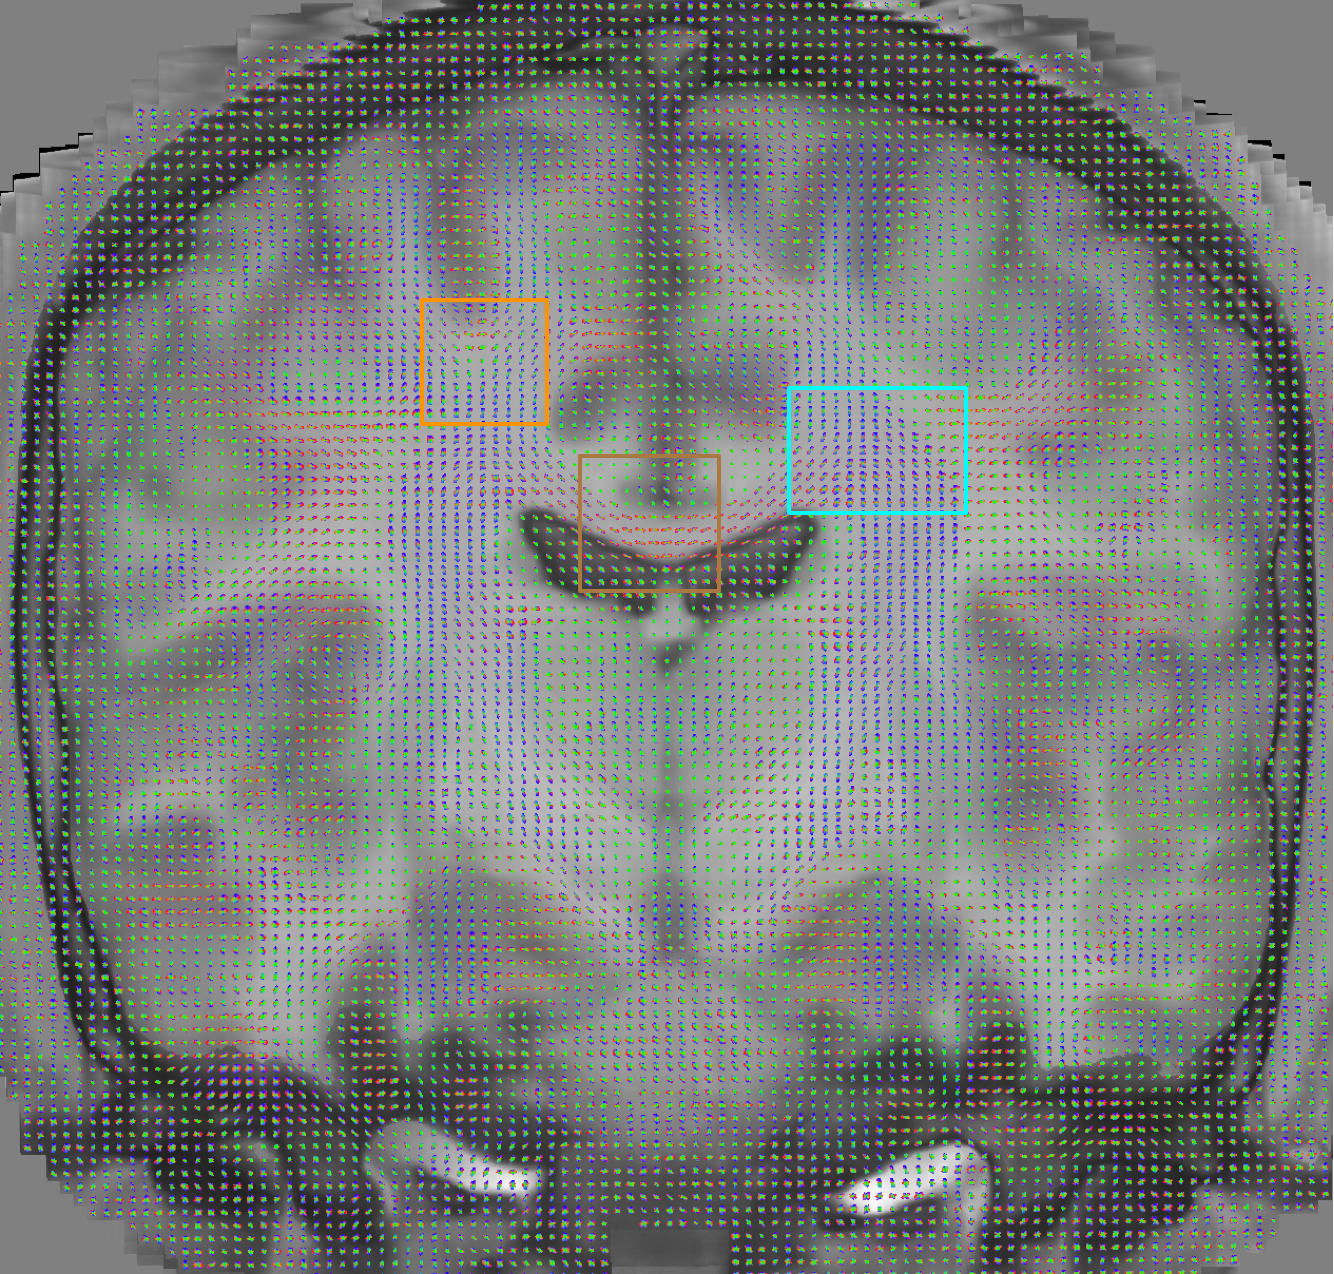
\includegraphics[width=0.7\linewidth, angle=0]{figs/Esquema_Glifo/Visual/Glifo_Fatia79_Coronal_front/coronal_glifos_lowRes_ft_cgcc_fan.png}
   \label{fig::multimodal_localizacao_coronal_1}
   }
    }
    \\
    \subfloat[relativa ao  axial]{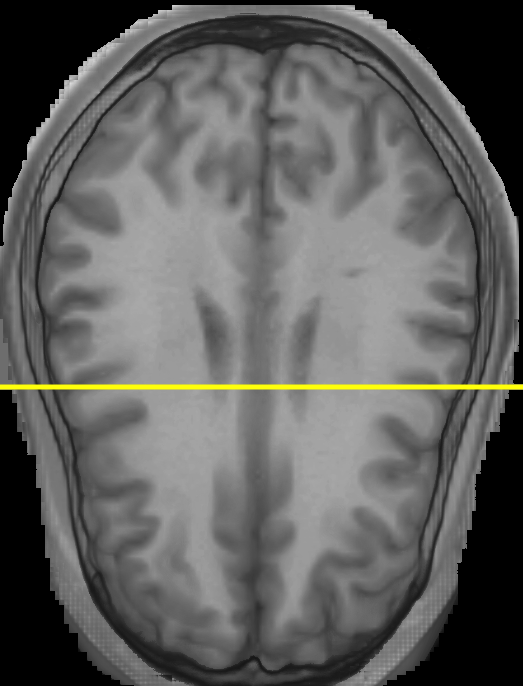
\includegraphics[width=.26\linewidth, angle=0]{figs/Esquema_Glifo/Visual/Glifo_Fatia79_Coronal_front/axial_marcado.png}
    \label{fig::multimodal_localizacao_axial_1}
    }
    \subfloat[relativa ao sagital] {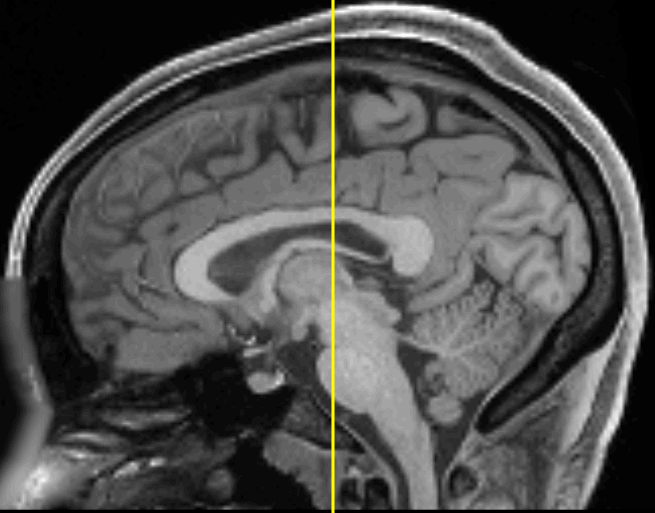
\includegraphics[width=.435\linewidth, angle=0]{figs/Esquema_Glifo/Visual/Glifo_Fatia79_Coronal_front/sagital_marcada.png}
    \label{fig::multimodal_localizacao_sagital_1}
    }
    \caption{Localização das regiões selecionadas numa fatia coronal.}
    \label{fig::multimodal_localizacao_1}
\end{figure}


A região destacada com a linha marrom na Fig. \ref{fig::multimodal_localizacao_coronal_1} corresponde à interface entre o corpo caloso e o cíngulo. Nesta região, temos uma configuração ``beijo'' (\textit{kissing}) entre os dois feixes de fibras.  Mais especificamente, os dois feixes se tocam perpendicularmente como mostra o esboço na Fig. \ref{fig::relacoes_espaciais_feixes}. Espera-se, portanto, que existam amostras na interface entre os dois feixes de fibras com duas direções de difusão dominantes, como revelam os glifos ODF destacados pelos retângulos marrons na Fig. \ref{fig::multimodal_cgcc_glifo_odf}. No entanto, os correspondentes glifos superquádricos na Fig. \ref{fig::multimodal_cgcc_superquadric}, também destacados pela linha marrom, assumem formas que nos induzem a concluir equivocadamente que as difusões sejam isotrópicas nas amostras destacadas. 
%nas visões axial e coronal , são apresentados nas Figs. \ref{???}, \ref{fig::multimodal_localizacao_1} e \ref{fig::multimodal_localizacao_2}.

%\subfloat[Fatia coronal de um MRI T1 co-registrado com DWI com glifos ODF sobrepostos. O glifos utilizam a $2^a$ ordem de tesselação do icosaedro. A região de Fig. \ref{fig::multimodal_cruzamento_1} está destacada em amarelo. A região em Fig. \ref{fig::multimodal_cgcc} está destacada em marrom]

%\todo[inline]{São 3 ou 4 regiões na Fig. 4.14.(a). Não dá para simplesmente incluir um texto sem avaliar o impacto! Onde fica os glifos destacados pelo contorne magenta na Fig. 4.15?}


%\subsection{Fibras na região delimitadas pelo centro semioval}
%\label{ssec::fibras_que_passam}

% evidencia uma melhora na tractografia do trato corticoespinhal, contido na \textit{corona radiata} através de um método de alta ordem (\textit{Q-Ball Imaging}) em relação ao DTI, fazendo a validação via com estimulação cortical. SLF!!!. Corpo Caloso. cíngulo HARDI.

%Para certificar o cruzamento dos três feixes de fibras, quase perpendiculares entre si, no centro semioval, analisamos ainda comparativamente os glifos ODF e superquádricos renderizados na fatia axial da Fig. \ref{fig::multimodal_localizacao_axial_1}. Fig. \ref{fig::multimodal_localizacao_2} mostra a posição anatômica da fatia selecionada, como também o foco de exploração, destacado pela linha amarela. A região de foco contém uma linha de glifos dentro da área contornada pela linha amarela na Fig. \ref{fig::multimodal_localizacao_coronal_1}. 

%\begin{figure}[H]
%\centering
%\captionsetup[subfloat]{farskip=0pt,nearskip=0pt}
    %\rule{6cm}{3cm}
%    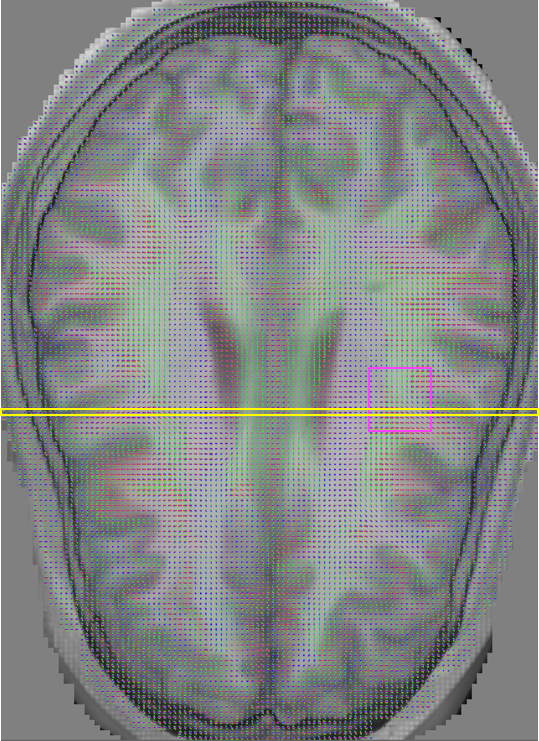
\includegraphics[width=1.\linewidth, angle=0]{figs/Esquema_Glifo/Visual/Glifo_Fatia78_Axial_Top/low_res_glifo_marcado_tf.png}
%    \caption{Visualização de glifos na fatia axial da Fig.\ref{fig::multimodal_localizacao_axial_1}. A região no centro semioval destacada em magenta está em Fig. \ref{fig::multimodal_cruzamento_2}. O contorno amarelo indica a fatia coronal em Fig. \ref{fig::multimodal_localizacao_coronal_1}}
%    \label{fig::multimodal_localizacao_2}
%\end{figure}




%Fig. \ref{fig::multimodal_cgcc} destaca em marrom uma região em que temos uma configuração ``beijo'' de dois feixes de fibras perpendiculares entre si, em Fig. \ref{fig::multimodal_localizacao_1} em uma visão coronal. Fig. \ref{fig::multimodal_cgcc_glifo_odf} mostra a região com glifos ODF e \ref{fig::multimodal_cgcc_superquadric} ilustra a região com superquádricos.

 \begin{figure}[H]
\centering
%\captionsetup[subfloat]{farskip=0pt,nearskip=0pt}
    %\rule{6cm}{3cm}
    \subfloat[Glifos ODF do GQI.]{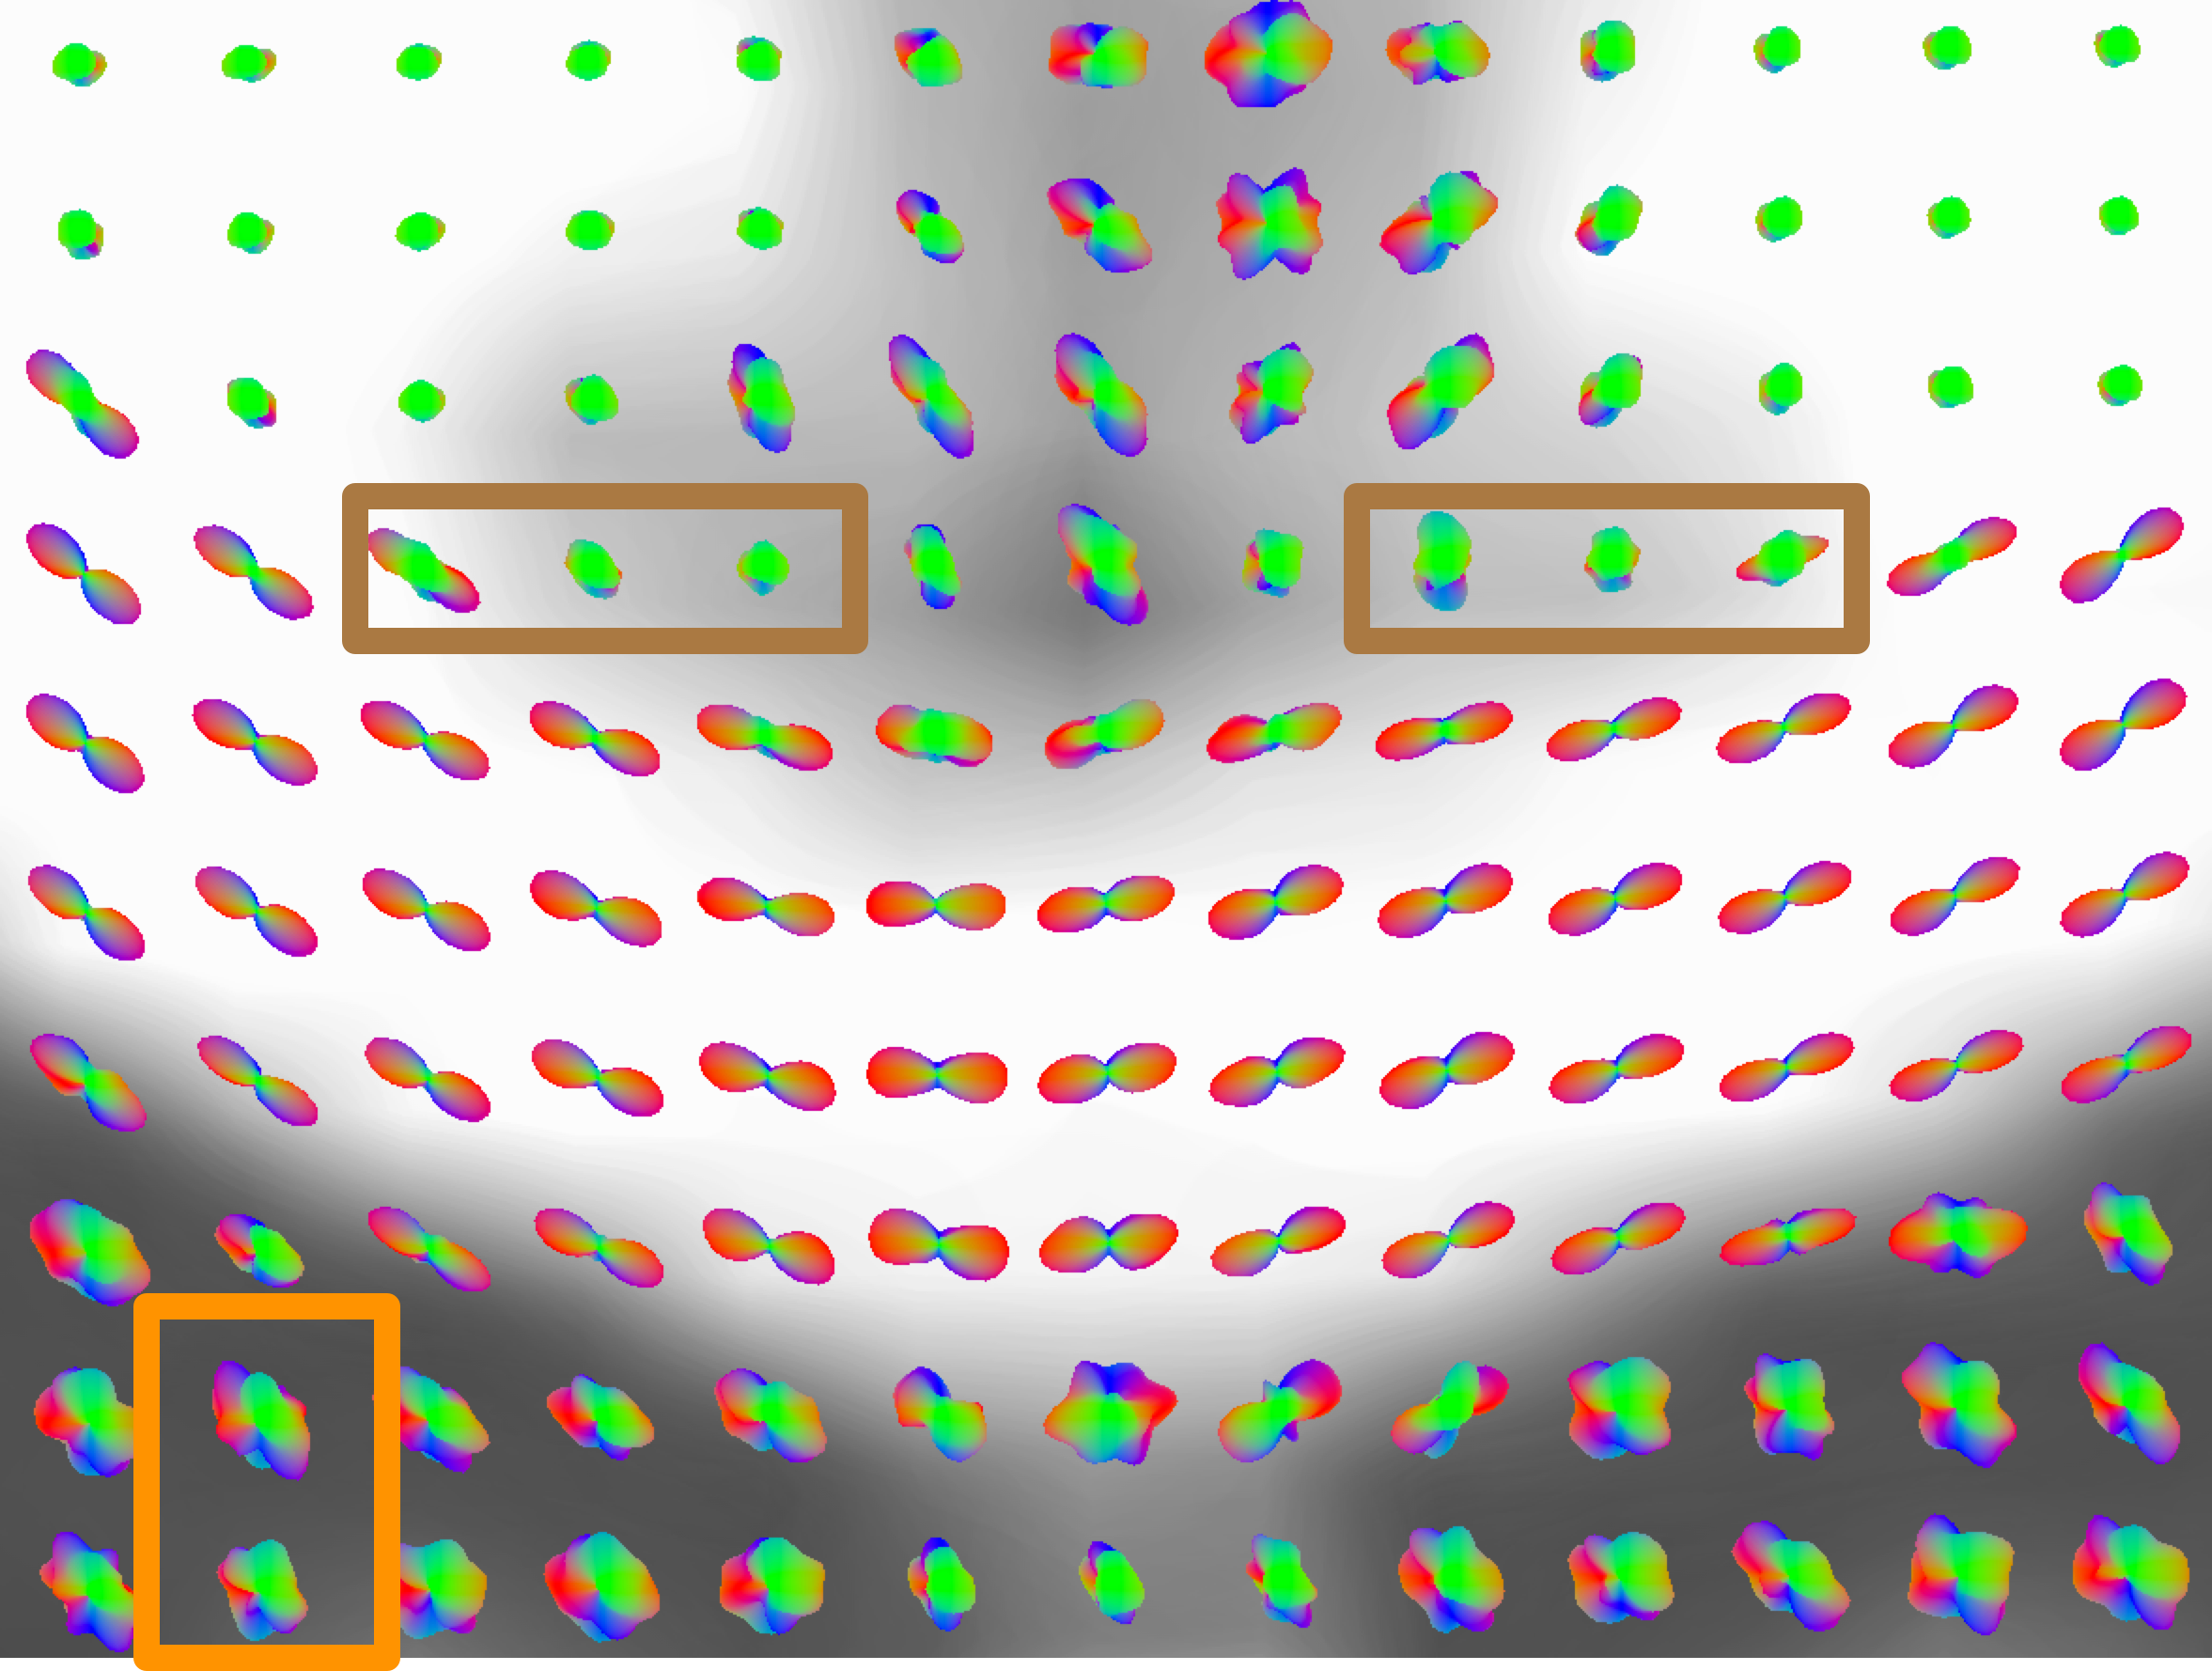
\includegraphics[width=.47\linewidth, angle=0]{figs/Esquema_Glifo/Visual/CG_CC/glifo_ODF_marcado_3.png}
    \label{fig::multimodal_cgcc_glifo_odf}
    }
    \subfloat[Superquádricos.] {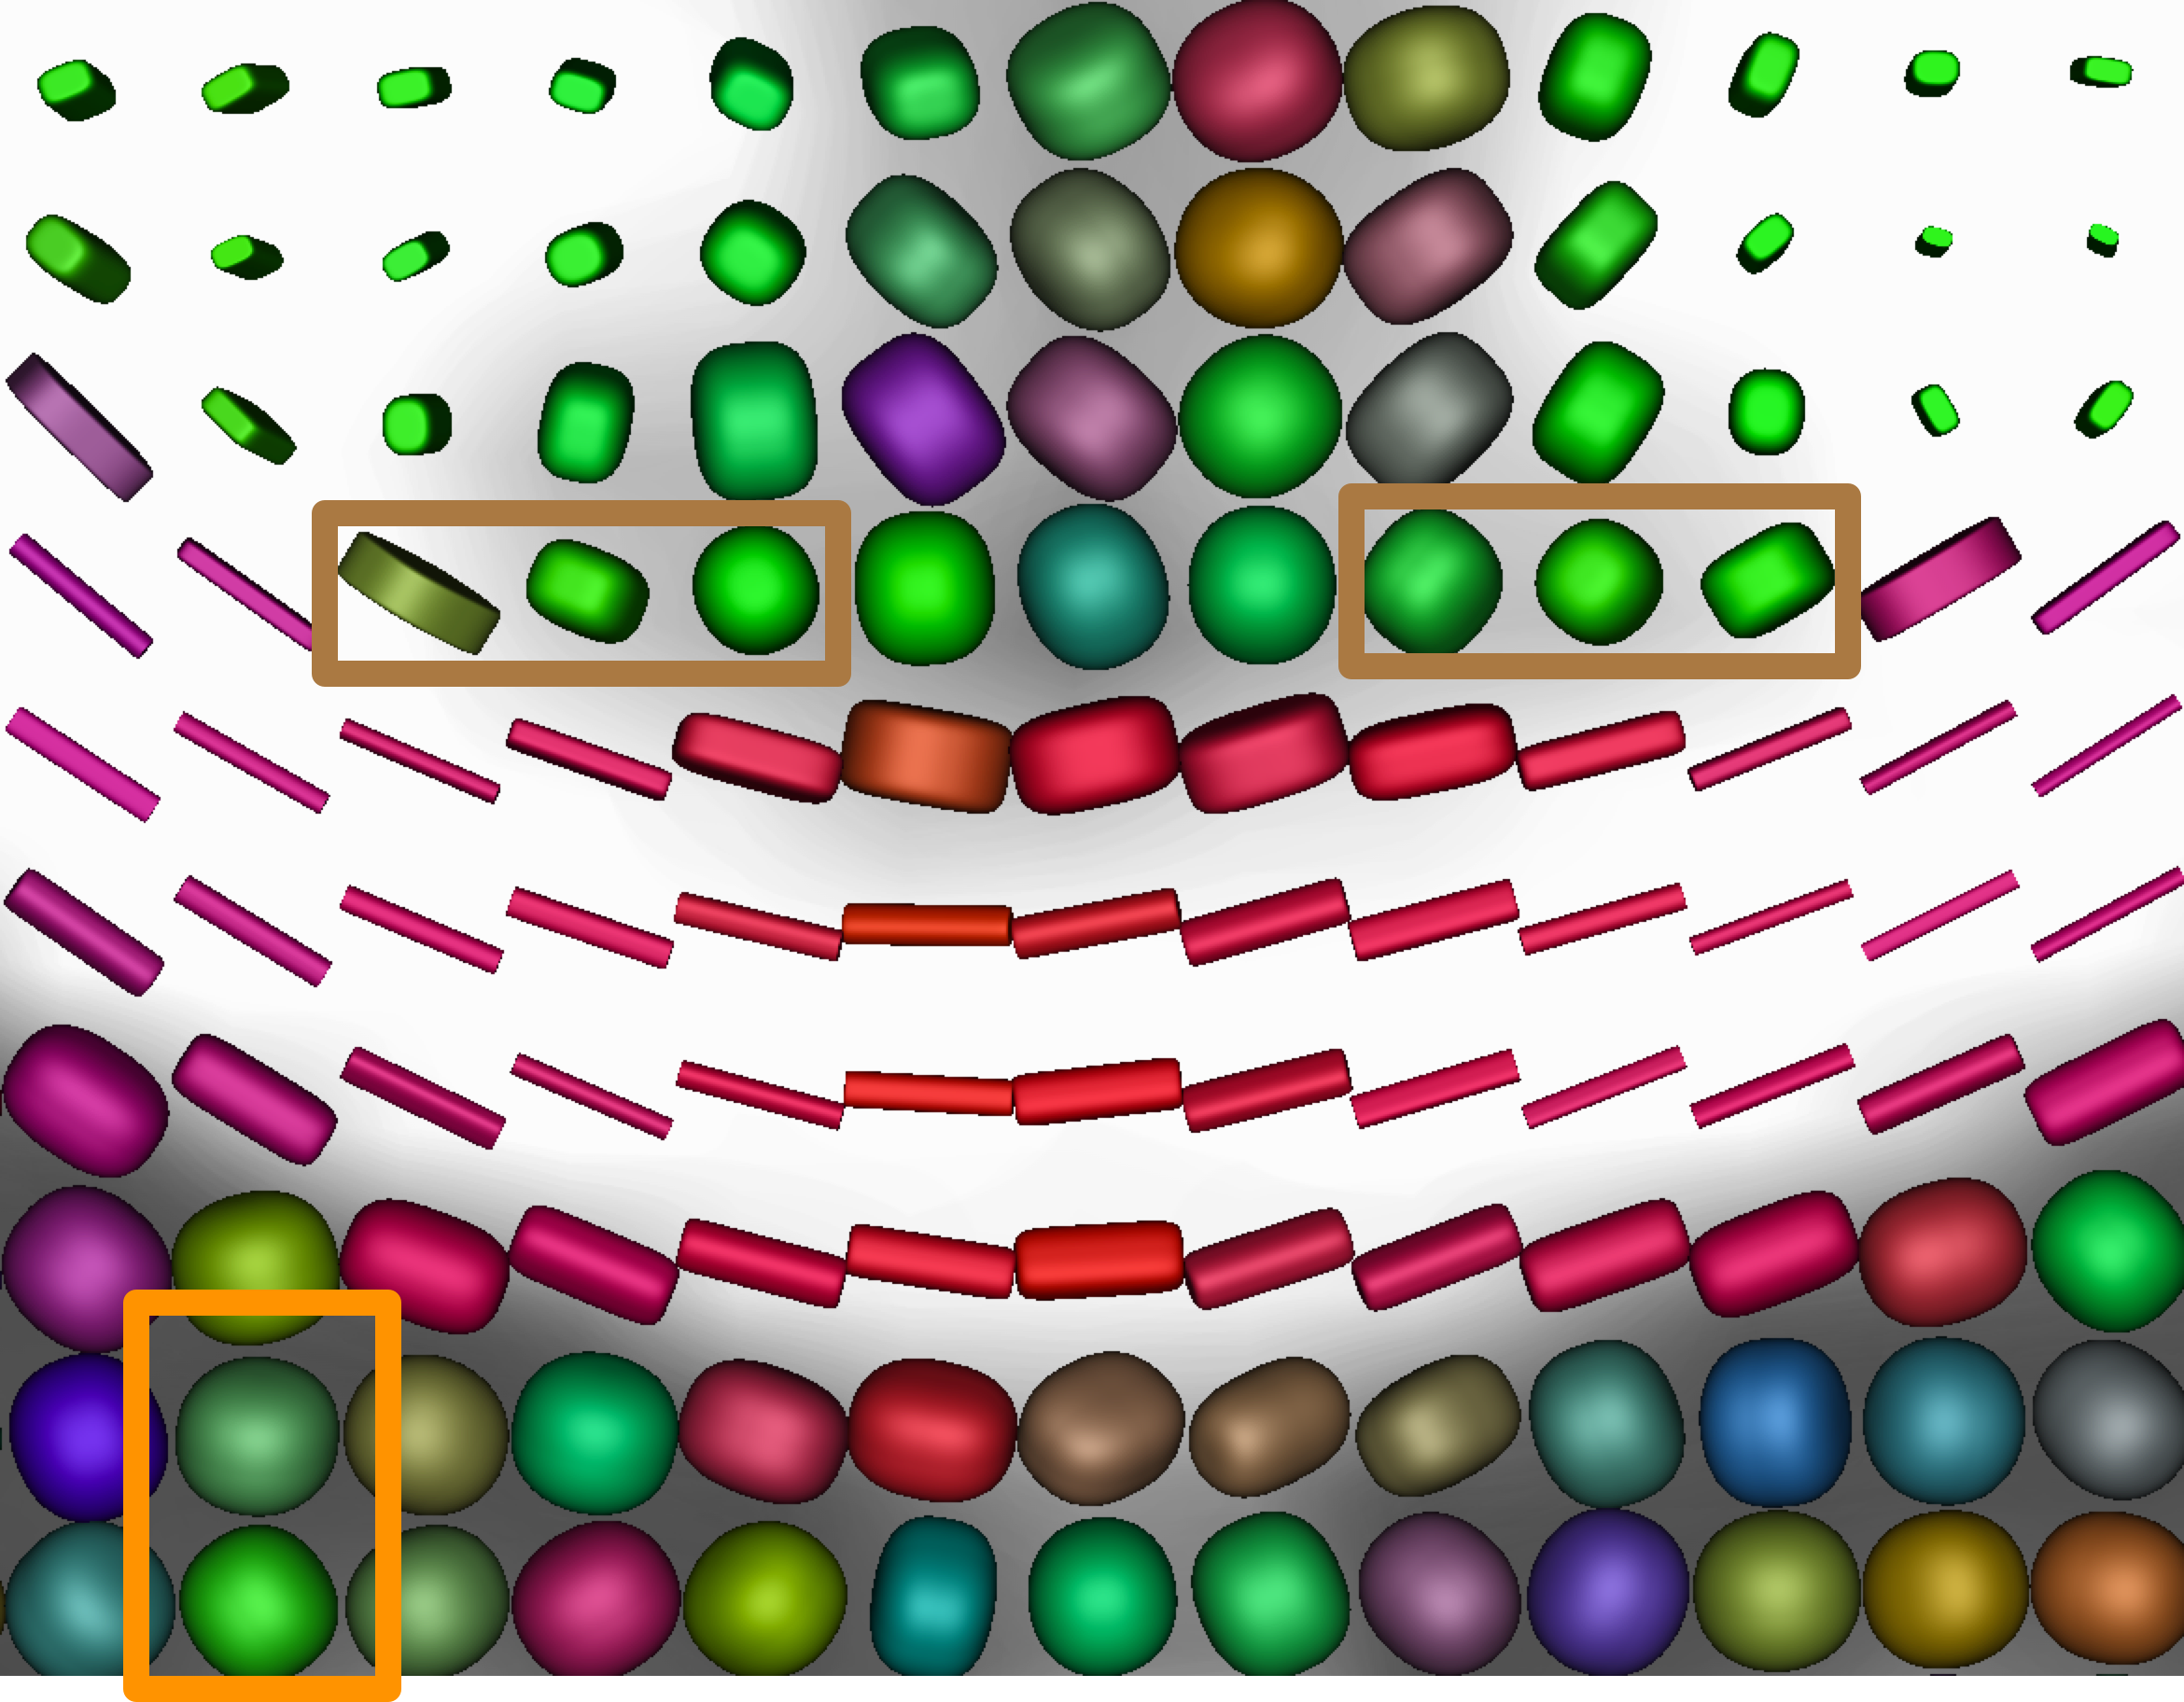
\includegraphics[width=.47\linewidth, angle=0]{figs/Esquema_Glifo/Visual/CG_CC/superquadrico_marcado_3.png}
    \label{fig::multimodal_cgcc_superquadric}
    }
    \caption{``Beijo'' na interface entre cíngulo e corpo caloso.% região de cruzamento da \textit{corona radiata}, corpo caloso e fascículo longitudinal superior em uma visão coronal.
    }
    \label{fig::multimodal_cgcc}
\end{figure}

A região destacada com a linha preta na Fig. \ref{fig::multimodal_fanning_glifo_odf} corresponde à base de um leque de fibras que passam pela cápsula interna. Nesta região, temos uma configuração ``leque'' (\textit{fanning}) de axônios que conectam a cápsula interna com o córtex cerebral, a camada mais externa do cérebro. Entre os feixes de fibras que passa pela cápsula interna está o trato cortico-espinhal ilustrado na Fig. \ref{fig::relacoes_espaciais_feixes}. Espera-se, portanto, que existam amostras nesta região com duas direções dominantes oblíquas, e não perpendiculares entre si como na interface cíngulo--corpo caloso. Os glifos destacados pela linha preta na Fig. \ref{fig::multimodal_fanning_glifo_odf} tem uma componente azul (direção ascendente) e magenta (direção diagonal entre ascendente e lateral) dominantes. Os glifos superquádricos correspondentes, na Fig. \ref{fig::multimodal_fanning_superquadric}, apresentam formas tubulares tendo somente ou a direção ascendente ou a direção diagonal entre ascendente e lateral como dominante. % \textcolor{magenta}{indicando que a segunda direção de difusão dominante é perpendicular ao plano da fatia.}%Comparando esses glifos com os seus correpondentes glifos superquádricos na Fig. \ref{fig::multimodal_fanning_superquadric}...

 \begin{figure}[H]
\centering
%\captionsetup[subfloat]{farskip=0pt,nearskip=0pt}
    %\rule{6cm}{3cm}
    \subfloat[Glifos ODF do GQI.]{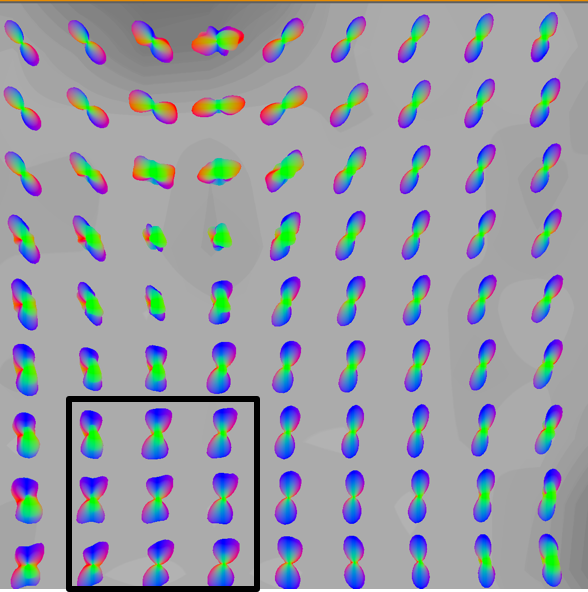
\includegraphics[width=.47\linewidth, angle=0]{figs/Esquema_Glifo/Visual/Fanning/glifo_ODF_marcado_4.png}
    \label{fig::multimodal_fanning_glifo_odf}
    }
    \subfloat[Superquádricos.] {\includegraphics[width=.47\linewidth, angle=0]{figs/Esquema_Glifo/Visual/Fanning/superquadrico_marcado_4.png}
    \label{fig::multimodal_fanning_superquadric}
    }
    \caption{Bifurcação de fibras no trato cortico-espinhal.% região de cruzamento da \textit{corona radiata}, corpo caloso e fascículo longitudinal superior em uma visão coronal.
    }
    \label{fig::multimodal_fanning}
\end{figure}

Finalmente, a região destacada com a linha ciano na Fig. \ref{fig::multimodal_localizacao_coronal_1} faz parte do centro semioval, onde ocorre o cruzamento de três grandes feixes de fibras, SLF, CC e CS, como ilustra a Fig. \ref{fig::tratos}. Enquanto os glifos superquádricos correspondentes tem a forma de disco, ou uma forma retangular suave, como se houvessem somente duas direções dominantes de difusão (Fig. \ref{fig::multimodal_superquadric_1}), os glifos ODF mostram nitidamente cruzamentos de duas ou três direções. Os cruzamentos entre CS e CC ocorrem de forma oblíqua no plano da imagem e o SLF II, que é normal ao plano da imagem, cruza com CS e CC perpendicularmente (Fig. \ref{fig::multimodal_glifo_odf_1}). O glifo ODF destacado pela linha preta, que possui três direções de difusão dominantes, é ilustrado nos três planos anatômicos na Fig. \ref{fig::multimodal_cruzamento_2}. 

% Nesta figura, as direções dos glifos contornados pela linha preta são paralelas às direções anatômicas, medio--lateral (vermelho), inferior--superior (azul), e antero--posterior (verde), evidenciando \sout{a ortogonalidade}\textcolor{red}{o cruzamento} dos feixes de fibras subjacentes. Os glifos superquádricos, associados às mesmas amostras na\sout{s} Fig\sout{s}. \ref{fig::multimodal_superquadric_1} \sout{e \ref{fig::multimodal_superquadric_2},} não permite\sout{m} inferir esse cruzamento (\textit{crossing}) de 3 feixes.

%\sout{Fig. \ref{fig::multimodal_localizacao_1} ilustra a localização da região de análise em amarelo a ser observada em Fig. \ref{fig::multimodal_cruzamento_1}, na qual provê uma visão coronal dos cruzamentos.  mostra a região com glifos ODF e \ref{fig::multimodal_superquadric_1} mostra a região com superquádricos.
%}

%\sout{
%Por sua vez, Fig. \ref{fig::multimodal_localizacao_2} ilustra a localização da região de análise a ser observada em Fig. \ref{fig::multimodal_cruzamento_2} e provê uma visão axial dos cruzamentos. Assim como na visão coronal, Fig. \ref{fig::multimodal_glifo_odf_2}  mostra a região com glifos ODF e \ref{fig::multimodal_superquadric_2} mostra a região com superquádricos em uma visão axial. %Em Fig. \ref{fig::multimodal_glifo_odf_zoom}, ilustramos os glifos de ambas Fig. \ref{fig::multimodal_glifo_odf_1} e \ref{fig::multimodal_glifo_odf_2} contidas no quadrado pontilhado laranja a um fator de escala maior.
%}

 \begin{figure}[H]
\centering
%\captionsetup[subfloat]{farskip=0pt,nearskip=0pt}
    %\rule{6cm}{3cm}
    \subfloat[Glifos ODF do GQI.]{\includegraphics[width=.8\linewidth, angle=0]{figs/Esquema_Glifo/Visual/Glifo_Fatia79_Coronal_front/glifo_ODF_marcado.png}
    \label{fig::multimodal_glifo_odf_1}
    }
    \\
    \subfloat[Superquádricos.] {\includegraphics[width=.8\linewidth, angle=0]{figs/Esquema_Glifo/Visual/Glifo_Fatia79_Coronal_front/superquadrico_crossing.png}
    \label{fig::multimodal_superquadric_1}
    }
    \caption{Cruzamento no centro semioval numa fatia coronal.% região de cruzamento da \textit{corona radiata}, corpo caloso e fascículo longitudinal superior em uma visão coronal.
    }
    \label{fig::multimodal_cruzamento_1}
\end{figure}


%  \begin{figure}[H]
%  %\subfigcapskip = -5pt
%      \centering
%      \includegraphics[width=.7\linewidth, angle=0]{figs/Esquema_Glifo/Visual/Glifo_Fatia79_Coronal_front/coronal_lowRes.png}
%       \caption{Fatia coronal de um MRI T1 co-registrado com DWI. A malha esférica base corresponde a $2^a$ ordem de tesselação do icosaedro.}
%       \label{fig::multimodal_cruzamento_mapa_1}
%   %   \hspace{1pt}
%  \end{figure}

%  \begin{figure}[H]
%  %\subfigcapskip = -5pt
%      \centering
%      \includegraphics[width=.7\linewidth, angle=0]{figs/Esquema_Glifo/Visual/Glifo_Fatia79_Coronal_front/coronal_glifos_lowRes.png}
%       \caption{Fatia coronal de um MRI T1 co-registrado com DWI. A malha esférica base corresponde a $2^a$ ordem de tesselação do icosaedro.}
%       \label{fig::multimodal_cruzamento_mapa_glifos_1}
%   %   \hspace{1pt}
%  \end{figure}

 
 %\begin{figure}[H]
%\centering
%\captionsetup[subfloat]{farskip=0pt,nearskip=0pt}
    %\subfloat[Fatia coronal de um MRI T1 co-registrado com DWI. A malha esférica base corresponde a $2^a$ ordem de tesselação do icosaedro. A região delimitada pelo retângulo branco consiste no cruzamento de fibras ilustrado em Fig. \ref{fig::multimodal_cruzamento_1}]{\includegraphics[width=.80\linewidth, angle=0]{figs/Esquema_Glifo/LowResImgHighlighted.png}
    %\label{fig::multimodal_lowres}
    %}
    %\hspace{1pt}
    
    %\subfloat[Cruzamento entre fibras de corpo caloso (esquerda-direita), \textit{corona radiata} (descendente-ascendente) e fascículo longitudinal superior (anteroposterior - normal ao plano da página). A malha esférica base é a $8^a$ ordem de tesselação do icosaedro.] %{\makebox[2.0\width]
    %{\includegraphics[width=.45\linewidth, angle=0]{figs/Esquema_Glifo/HighResImg.png}
    %\label{fig::multimodal_highres}}
    %%}
    %\caption{Glifos ODF integrados ao ambiente de visualização multimodal para MRI. A imagem se refere a um MRI T1 cor-registrado a o seu respectivo DWI. %\ref{fig::multimodal_highres} corresponde a região dentro do contorno de cor branca em \ref{fig::multimodal_lowres}.}
    %\label{fig::multimodal}
%\end{figure}
 

%\todo[inline]{Talvez seja interessante em destacar os glifos ODFs com mais pontas ... Não dá para perceber nas figuras. Use por exemplo o package tikz. Acho que o Wallace usou muito na tese dele ...}

%\textcolor{red}{Mostraremos comparativamente as imagens com os glifos superquádricos geradas com as imagens selecionadas na seção \ref{ssec::reais_resultados}.}

% Observe também que a resolução do glifo é diferente na Fig. \ref{fig::multimodal_lowres} em comparação a \ref{fig::multimodal_highres} e sua seleção é feita de forma automática. No fundo, há a renderização da ressonância anatômica ponderada em T1 co-registrada.

%\todo[inline]{\textcolor{green}{Destacar glifos importantes}}

%  \begin{figure}[H]
%  %\subfigcapskip = -5pt
%      \centering
%      \includegraphics[width=.7\linewidth, angle=0]{figs/Esquema_Glifo/Visual/Glifo_Fatia78_Axial_Top/low_res_marcado.png}
%       \caption{Fatia coronal de um MRI T1 co-registrado com DWI. A malha esférica base corresponde a $2^a$ ordem de tesselação do icosaedro.}
%       \label{fig::multimodal_cruzamento_mapa_2}
%   %   \hspace{1pt}
%  \end{figure}


%  \begin{figure}[H]
%  %\subfigcapskip = -5pt
%      \centering
%      \includegraphics[width=.7\linewidth, angle=0]{figs/Esquema_Glifo/Visual/Glifo_Fatia78_Axial_Top/low_res_glifo_marcado.png}
%       \caption{Fatia coronal de um MRI T1 co-registrado com DWI. A malha esférica base corresponde a $2^a$ ordem de tesselação do icosaedro.}
%       \label{fig::multimodal_cruzamento_mapa_glifos_2}
%   %   \hspace{1pt}
%  \end{figure}
 
%\todo[inline]{Eu removeria Fig. 4.19. Não acrescenta nada. Só confunde mais.}


 \begin{figure}[H]
\centering
%\captionsetup[subfloat]{farskip=0pt,nearskip=0pt}
    %\rule{6cm}{3cm}
    \subfloat[Coronal] {\includegraphics[width=.20\linewidth, angle=0]{figs/Esquema_Glifo/Visual/Glifo_Fatia79_Coronal_front/glifo_cruzamento/coronal.png}
    \label{fig::glifo_cruzamento_coronal}
    }
    \subfloat[Axial] {\includegraphics[width=.20\linewidth, angle=0]{figs/Esquema_Glifo/Visual/Glifo_Fatia79_Coronal_front/glifo_cruzamento/axial.png}
    \label{fig::glifo_cruzamento_axial}
    }
    \subfloat[Sagital] {\includegraphics[width=.24\linewidth, angle=0]{figs/Esquema_Glifo/Visual/Glifo_Fatia79_Coronal_front/glifo_cruzamento/sagital.png}
    \label{fig::glifo_cruzamento_sagital}
    }
    \caption{Detalhes do glifo, destacado na Fig. \ref{fig::multimodal_glifo_odf_1}, num \textit{voxel} onde ocorre o cruzamento entre CS (azul, ascendente inclinado para esquerda), CC (azul, ascendente inclinado para direita)  SLF (anteroposterior, verde).}
    \label{fig::multimodal_cruzamento_2}
\end{figure}


\subsection{Discussões}
\label{ssec::visual_discussoes}

%\todo[inline]{Revise integralmente o texto. Os glifos mostrados no link realçam melhor as direções (fODFs)! \url{http://cmic.cs.ucl.ac.uk/cdmri10/invited_tournier.pdf}. É preciso levar em conta nas discussões \textcolor{green}{Levei em consideração, mencionei as diferentes naturezas das dODF e as ODFs do CSD}}
%\todo[inline]{\textcolor{green}{Adicionei a seção 4.5.2.2 para ilustrar o exemplo que ele mostra com SD}}

\todo[inline]{O que você quer discutir sobre os resultados obtidos? O poder informativo quanto à visualização e análise das difusões intravóxeis e intervóxeis? Como este poder é demonstrado através das imagens selecionadas?}

Na Fig. \ref{fig::multimodal_cgcc}, os glifos destacados em marrom consistem em transições entre cíngulo e corpo caloso. Observe que, a partir dos glifos superquádricos na Fig. \ref{fig::multimodal_cgcc_superquadric}, não é possível inferir sobre a direção das fibra subjacentes. Esses superquádricos se parecem com alguns glifos dos ventrículos, contornados pela linha em laranja, onde a difusão é isotrópica. Por outro lado, os glifos ODF, contornados pela linha marrom na Fig. \ref{fig::multimodal_cgcc_glifo_odf}, apresentam formas diferenciadas das formas dos glifos na região isotrópica. Eles mostram nitidamente as duas direções associadas ao corpo caloso (vermelho em direção lateral) e ao cíngulo (verde em direção anteroposterior), que são diferentes dos glifos de múltiplas pontas difusas que caracterizam difusões intravóxeis isotrópicas. Por subestimar as direções de difusão intravóxel, os glifos superquádricos podem proporcionar uma noção equivocada das relações intervóxeis e levar a entendimento de conexões incorretas entre regiões corticais.% \sout{Adicionalmente, podemos visualizar que há uma correlação intervoxel para os glifos localizados na região de transição, já que ambos podem ser interpretados como uma composição da região acima na imagem (CG) com a de baixo (CC).}


Embora de forma sutil, Fig. \ref{fig::multimodal_fanning} demonstra a capacidade dos glifos ODF em mostrar configurações em ``leque'' (\textit{fanning}), típica do trato cortico-espinhal \cite{fortin2012, wang2019}. Como já destacamos na Seção \ref{ssec::visual_resultados}, os glifos ODF contornados pela linha preta na Fig.\ref{fig::multimodal_fanning_glifo_odf} tem  direções predominantemente ascendentes e levemente inclinadas na direção lateral com uma cor que transita entre azul e magenta, evidenciando mais de uma direção de difusão. Com os glifos superquádricos, destacados na Fig. \ref{fig::multimodal_fanning_superquadric}, não há a possibilidade de inferência sobre a abertura em ``leque'' por serem de formato tubular com tons de cor que variam entre magenta e azul. Vale ressaltar que há coerência, tanto em cor quanto em forma, entre os glifos ao lado da região de abertura em ``leque'' destacada. A diferença ocorre no meio da abertura, onde somente os glifos ODFs conseguem revelar a existência de uma região de mistura das duas direções de difusão.

Nos \textit{voxels} do centro semioval, ilustrados na Fig. \ref{fig::tratos},  temos um cruzamento entre o corpo caloso, que vem da parte medial do cérebro,
o trato cortico-espinhal, que tem direção dominantemente ascendente vindo da cápsula interna, e o fascículo longitudinal superior, que tem direção anteroposterior. Pode-se perceber pela Fig. \ref{fig::multimodal_cruzamento_1} que, 
enquanto as pontas isoladas, ou os máximos locais, dos glifos ODF (Fig. \ref{fig::multimodal_glifo_odf_1}, e também Fig. \ref{fig::multimodal_cruzamento_2}) permitem inferir sobre a natureza do cruzamento, os superquádricos, por apresentarem uma forma retangular suave ou em disco (Fig. \ref{fig::multimodal_superquadric_1}), não conseguem proporcionar uma noção de cruzamento. As pontas dos glifos ODFs indicam as prováveis direções de cada feixe de fibras de forma mais precisa. Adicionalmente, constatamos com a Fig. \ref{fig::multimodal_cruzamento_2} uma observação de \citeonline{dellacqua2019} acerca a angulação de cruzamento entre os feixes de fibras de 0$^o$ a 90$^o$: quanto maior a angulação, mais delineadas são as pontas associadas aos feixes. Como a angulação de cruzamento entre CC e CS é menor que 90$^o$ no glifo destacado (Fig. \ref{fig::multimodal_cruzamento_2}), o conjunto de pontas ascendentes e inclinadas para direita (CC) e esquerda (CS) (Fig. \ref{fig::glifo_cruzamento_coronal}) é menos distinguível no glifo que o cruzamento das pontas de CC e CS com as pontas de cor verde (SLF).


Cabe aqui uma ressalva aos resultados da nossa análise. Embora seja possível identificar visualmente, através das formas e das cores dos glifos ODF implementados, a presença de configurações de múltiplas direções de difusão intravoxel, as características aplicadas são somente condições necessárias. Elas não são suficientes para distinguirmos as diferentes configurações. Essa questão é um problema ainda em aberto \cite{SCHILLING2019194} e não é tratada no escopo deste projeto.

%\sout{Nos glifos ODF do centro semioval, ilustrado na Fig. \ref{fig::multimodal_glifo_odf_1}, temos um cruzamento entre o corpo caloso e que vem da parte medial do cérebro, representado na parteinferior esquerda da imagem e tem uma direção na diagonal ascendente e lateral, e as fibrasdo trato CS, que tem direção dominantemente ascendente, vindo da cápsula interna, na parte inferior direita na imagem e o SLF II, que tem direção anteroposterior e está normalao plano da imagem e é predominante na parte superior direita da imagem. Pode-se perceber na região de cruzamento de fibras que, enquanto nos glifos ODF é possível inferir sobre a natureza do cruzamento, os superquádricos apresentam uma forma retangular suave ou disco e não geram a possibilidade de inferimento sobre as fibras que compõem o cruzamento. Através dos glifos ODF, é possível inferir sobre as regiões que são delimitadas pelos tratos. Tomando como exemplo o SLF II, é possível inferir sobre a localização das fibras do trato a partir de componentes verdes dominantes nos glifos ODF na partesuperior direita da imagem, mas a partir dos superquádricos, há glifos na região com tons de cor vermelha e cor de ferrugem (Fig. \ref{fig::multimodal_superquadric_1}) que evidenciam uma descorrelação daaparência do glifo com a vizinhança.
%}

\citeonline{daducci2014} mostraram que se pode inferir direções de fibras subjacentes à amostras de difusão de um \textit{voxel} pelos máximos locais de dODFs. Isso permite a estimativa das orientações de fibras nervosas através dos máximos locais das funções de distribuição de orientações de difusão (dODFs) \cite{descoteaux2007, chamberland2014}, de forma análoga ao cômputo de autovetores a partir dos tensores de difusão (DTI), para rastrear uma fibra a partir de uma semente pela técnica de reconstrução conhecida por \textit{streamline fiber tractography} \cite{Mori1999}. Com a vantagem de ter mais opções de direção de difusão em cada amostra em relação a DTI, dODFs permitem, por exemplo, a reconstrução de feixes do CS que se ramifiquem em sua totalidade na região do giro pré e pós-central, conhecida por homúnculo de Penfield \cite{wang2019}, ao invés de uma reconstrução incompleta como apresentada na Fig. \ref{fig::tratos_1} \cite{bucci2013}. Ademais, baseado nos estudos conduzidos por \citeonline{voltoline2021}, acreditamos que a visualização dos glifos ODF possam contribuir na escolha mais precisa de uma região de sementes.

%\sout{Em algoritmos de tractografia baseados em rastreamento de linhas (\textit{streamline fiber tractography}) que utilizam o DTI, o fato do tensor de difusão não modelar a abertura em ``leque'' de fibras faz com que os feixes não se ramifiquem em sua totalidade na região do giro pré e pós-central, conhecida por homúnculo de Penfield. Isso corrobora com os resultados registrados na literatura \cite{bucci2013} e na reconstrução em Fig. \ref{fig::tratos_1}. Por sua vez, técnicas de tractografia de rastreamento de linhas baseadas em dODFs conseguem reconstruir fibras do CS que se ramificam em uma área maior no giro pré e pós-central \cite{wang2019}.
%}

%As dODFs permitem gerar feixes do CS que se ramifiquem em direção a  de uma enquanto há uma subestimação na bifurcação das fibras em técnicas baseadas em DTI, como mostrado nas Fig. \ref{fig::tratos_1} e \ref{fig::tratos_2}.

%Salientamos que a coroa radiada é uma das mais complexas regiões a se inferir sobre a matéria branca no cérebro, pois há muitas configurações de fibras que se cruzam e que se abrem em ``leque'' \cite{schilling2017}.


%Observe que no cruzamento entre os tratos, é possível inferir sobre as componentes ascendentes e que seguem na direção diagonal, porém quando o ângulo entre ambos tratos diminui, a distinguibilidade piora.
%Adicionalmente, observe na região delineada pelo contorno amarelo que há uma forte componente de cor verde, que na figura está normal à ao plano da imagem, indicando que há um ``beijo'' entre o cíngulo com o corpo caloso, que nesta região assume uma direção ascendente.
%No canto superior direito há glifos que tem um direção dominante anteroposterior, que são derivados do SLF, que iremos analisá-los na Fig. \ref{fig::multimodal_glifo_odf_2}.

%Nos glifos ODF do centro semioval numa visão axial, ilustrado na Fig. \ref{fig::multimodal_glifo_odf_2}, é possível notar que há regiões que pode-se inferir acerca do cruzamento de fibras. Há uma direção dominante no eixo $y$ de cor verde, que se refere ao SLF e outra de cor vermelha perpendicular, que se refere ao corpo caloso. A esquerda, os glifos em azul estão normais ao plano da imagem e se referem a fibras do trato CS em direção ascendente.

%Podemos comparar as imagens com os superquádricos, nos quais \citeonline{voltoline2021} evidenciaram que a sua respectiva renderização multimodal pode ajudar no processo de escolhas referentes a sementes em tractografia, em comparação à mapas de anisotropia codificados por cor. Fig. \ref{fig::multimodal_superquadric_1} ilustra a mesma região de Fig. \ref{fig::multimodal_glifo_odf_1} com superquádricos.



%Observe em Fig. \ref{fig::multimodal_superquadric_2} os superquádricos que estão no cruzamento de fibra entre SLF e corpo caloso e tem uma forma retangular suave que, ora apresentam uma cor dominante verde, vinculada a direção de difusão do SLF, ora apresentam uma cor dominante vermelha, vinculada ao corpo caloso. Podemos ver através dos glifos ODF que as cores vermelhas do cruzamento, localizadas na parte inferior da imagem no cruzamento estão vinculadas a uma probabilidade de difusão maior na direção $x$, associado ao corpo caloso. Adicionalmente, as cores verdes dos superquádricos, localizadas mais acima na imagem e destacadas pelo contorno preto no cruzamento, estão associadas a uma maior probabilidade de difusão na direção do SLF, que é ilustrado num maior alongamento da componente direcional na direção do eixo $y$ que em $x$ no glifo ODF.

%Na Fig. \ref{fig::multimodal_glifo_odf_zoom}, ilustramos glifos renderizados sob um fator de escala muito alto na região de cruzamentos de fibra.
%\sout{Em Fig. \ref{fig::multimodal_cruzamento_2}, observe que o cruzamento de fibra entre o SLF e o corpo caloso e cortico-espinhal é mais notável que o cruzamento entre o CC e CS. Isto evidencia o fato de que menor o ângulo de cruzamentos mais suave é a transição entre as componentes associadas a cada fibra geradas no glifo implicando em uma menor distinguibilidade na interpretação sobre as fibras subjacentes. A presença desta suavidade é característica das dODFs obtidas a partir dos métodos livres de modelo \cite{dellacqua2019}.}


%Adicionalmente, observe que a tesselação de oitava ordem do icosaedro (1280 triângulos) utilizada nas Fig. \ref{fig::multimodal_glifo_odf_1} e \ref{fig::multimodal_glifo_odf_2}  geram um glifos com uma superfície suave o suficiente para que a sua qualidade visual em resolução não se deteriore com o aumento do fator de escala.


%\sout{As regiões alongadas dos glifos ODF, a partir das quais inferimos sobre a distribuição subjacente de fibras, abrigam os máximos locais das dODFs, que são comumente utilizados para cômputo da distribuição de fibras subjacentes intravoxel e são utilizados em tractografia a partir de métodos de alta ordem \cite{descoteaux2007, chamberland2014}.}



%\sout{Mesmo dando a possibilidade de inferir sobre o perfil direcional de fibras subjacente através dos máximos locais \cite{daducci2014}, as dODFs não dão a possibilidade de inferimento sobre a configuração de coexistência de fibras intravoxel (``leque'', ``beijo'', cruzamento, torção) \cite{SCHILLING2019194} e isto é mapeado também nos glifos. Salientamos que os exemplos de cruzamento, ``beijo'' (\textit{kissing}) e abertura em ``leque'' mostrados levam conhecimentos anatômicos dos comportamentos das fibras a priori. Esta limitação, que não é particular dODFs mas aos métodos de alta ordem de forma geral, trazem limitações aos algoritmos de tractografia associados. A classificação quanto a natureza da configuração de coexistência de fibras intravoxel é uma questão em aberto \cite{SCHILLING2019194}.} %De forma geral, os máximos locais extraídos de dODFs/fODFs obtidas através métodos de alta ordem conseguem inferir bem sobre distribuição subjacente de fibras intravoxel, mas os métodos não dão informações acerca da configuração de coexistência das fibras nos \textit{voxels}, e 


%\textcolor{magenta}{Nesta seção, concluímos que a partir dos glifos, conseguimos ter a inferência sobre a direção de fibra a partir das ODF geradas por um método de imageamento de alta ordem, no qual usamos o GQI. Salientamos que os glifos evidenciam o comportamento de ODFs e que a sua interpretabilidade é intrínseca a aplicações de métodos de alta ordem para aquisições DWI. }

Para concluir, vale comentar que as abordagens baseadas em deconvolução esférica \cite{Tournier2004DirectEO, tournier2007} geram glifos mais delineados em relação às orientações de fibras do que os glifos ODF e outros glifos derivados de métodos livres de modelo \cite{dellacqua2019}. \citeonline{Yeh2013} mostraram, no entanto, que a regularização L$_2$ aplicada em métodos de deconvolução pode produzir fibras falsas e comprometer a especificidade dos glifos visualizados. Através de uma série de experimentos, eles concluíram que as funções de distribuição de orientações de fibras (fODFs) obtidas com as dODFs são mais acuradas do que as derivadas da deconvolução esférica.

%%%%%%%%%%%%%%%%%%%%%%%%%%%%%%%%%%%%%%%%%%%%%%


%\subsection{Renderização por Fatias}
%\label{ssec::renderizacao_por_fatias}

%Podemos comparar nossa abordagem com a de \citeonline{shattuck2008}, uma vez que ambas são baseadas em polígonos, onde amostras de ODF deformam uma malha esférica. Em sua abordagem, \citeonline{shattuck2008} armazena ODFs como coeficientes de funções base na CPU e os glifos são computados e visualizados em fatias, que são visualizadas de forma ortogonal. O cômputo da forma dos glifos é feito na CPU, onde o valor de ODF é computada para as normais dos vértices da malha esférica utilizada, deslocando cada um dos vértices, e o tráfego CPU-GPU consiste no envio de dados de vértices de forma que sua estrutura de dados define a superfície do glifo.

%Em nossa abordagem, setamos a malha esférica de amostragem a priori e armazenamos amostras de dados de ODF e mostramos estratégias para escolher a malha esférica adequada e estratégias para lidar com o gargalo de tráfego de dados CPU-GPU. Para atingir este objetivo, mostramos formas de organizar os dados de ODF e da malha esférica de amostragem para utilizar renderização por instâncias, técnica que não estava disponível quando \citeonline{shattuck2008} publicaram seu trabalho\footnote{Em OpenGL, renderização por instâncias foi disponibilizada a partir da versão 3.2, lançada em 2009}. Adicionalmente, no processo de renderização, apenas enviamos um conjunto de escalares de ODF para deslocar a malha esférica escolhida e deslocamos os pontos da malha nas \textit{threads} da GPU. Assim, o tráfego de dados por glifo é de $N/2 + (4-N/2 \mod{4})$ \textit{floats} para uma geometria base com $N$ vértices. A possibilidade de diminuir o tráfego de dados por glifo para esta quantidade tem sido crucial para renderizar este glifos com malhas suaves em taxas interativas. Adicionalmente, os glifos são renderizados com apenas um comando de desenho e sua quantidade máxima é limitada pelo máximo número de elementos permitidos em uma das dimensões da textura 2D.

%Uma vez que nossa abordagem é vinculada à renderização de um volume via \textit{ray-casting}, apenas os \textit{voxels} visíveis são requisitados a serem desenhados, e não há a restrição a uma fatia inteira. Além disso, no ambiente interativo de visualização, onde o usuário tem a possibilidade de mudar a escala e mover o volume, a detecção de \textit{voxels} visíveis certifica que os \textit{voxels} que estão fora da cena não são demandados na renderização, consequentemente, seus dados não são enviados à GPU e nem são processados no \textit{vertex shader} para serem descartados na rasterização.

%Nosso esquema é também aplicável em renderização de glifos baseada em fatia. Observe que, o conjunto $D$ pode se referir a um conjunto de índices referentes a \textit{voxels} que definem uma fatia. Adicionalmente, os atributos de translação podem posicionar os glifos em um \textit{grid} $W \times H$, onde este atributo posiciona cada objeto ao centro de cada célula, que é escalonado pelo fator que o faz estar contido.

%Objetivando gerar resultados de performance do algoritmo e renderização em uma fatia 2-D, fizemos o seguinte experimento: os eixos x e y são divididos em $H$ intervalos ($W = H$), gerando o total de $H^2$ células quadriculadas, no qual glifos são renderizados em cada uma delas. Cada glifo é escalonado para estar contido em sua respectiva célula e posicionado em seu centro. Fixamos a geometria base, assim como os atributos de translação e, para evidenciar a interatividade do algoritmo sob a circunstância de uma frequente troca de fatias, a cada requisição de desenho, os atributos de translação e a matriz de amostras de ODF são preparados e enviados à GPU, conforme mostrado na Subseção \ref{ssec::atributos}.

%Mensuramos o FPS como uma função da quantidade de glifos renderizados com $H$ variando de 5 até 100. O gráfico de $FPS \times \text{glifos renderizados}$ é ilustrado na Fig. \ref{fig::slice_benchmark} para diferentes geometria base utilizadas em uma janela $1200\times 1200$.

% \begin{figure}[h]
%     \centering
%     %\rule{6cm}{3cm}
%     \includegraphics[width=.65\linewidth, angle=0]{figs/Esquema_Glifo/benchmark_half_texopt.png}
%     \caption{FPS $\times$ quantidade de glifos renderizada. As cores azul, laranja, verde e vermelha correspondem a geometria base gerada pela $2^{a}$ $4^{a}$, $8^{a}$ e $16^{a}$ ordem de tesselação do icosaedro. Suas respectivas quantidades de vértices e triângulo são computadas nas Eq. \ref{eq::2ordem_icosphere_vertices} e \ref{eq::2ordem_icosphere_triangulos}, respectivamente.}
%     \label{fig::slice_benchmark}
% \end{figure}

%Os resultados indicam que nosso esquema dá resultados satisfatórios para uso interativo, e mostramos que é possível renderizar milhares de glifos em taxas interativas utilizando a $4^{a}$ ordem de tesselação do icosaedro e centenas com a malha suave gerada pela $16^{a}$ ordem de tesselação.

%Na próxima seção, descrevemos uma infra-estrutura fora do ambiente de renderização multimodal para renderização de glifos ODF no qual a utilizamos para fazer testes e validações da melhora do algoritmo. Nela, apresentamos o primeiro protótipo do algoritmo, no qual tem semelhanças com o trabalho de \citeonline{shattuck2008} e as funcionalidades adicionadas ao longo do tempo. Para mensurar ganhos obtidos para cada funcionalidade adicionada, mensuramos o FPS do algoritmo para diferentes quantidade de glifos renderizadas para diferentes resoluções e comparamos com à abordagem anterior.

%Objetivando gerar resultados de performance do algoritmo e renderização em uma fatia 2-D, fizemos o seguinte experimento: os eixos x e y são divididos em $H$ intervalos ($W = H$), gerando o total de $H^2$ células quadriculadas, no qual glifos são renderizados em cada uma delas. Cada glifo é escalonado para estar contido em sua respectiva célula e posicionado em seu centro. Fixamos a geometria base, assim como os atributos de translação e, para evidenciar a interatividade do algoritmo sob a circunstância de uma frequente troca de fatias, a cada requisição de desenho, os atributos de translação e a matriz de amostras de ODF são preparados e enviados à GPU, conforme mostrado na Subseção \ref{ssec::atributos}.


%, no qual foi aperfeiçoado por \cite{almsick2011}. Esta abordagem possibilitou incrementos em performance em relação a \citeonline{shattuck2008}.

%\citeonline{raphael_dissertacao} propôs um esquema de renderização interativa do tensor de difusão em glifos superquádricos \cite{Kindlmann2004} utilizando polígonos. Em seu trabalho, os glifos são renderizados a taxas interativas e a sua abordagem consiste na minimização de tráfego de dados entre CPU-GPU, que consiste apenas em parâmetros que customizam e deslocam os glifos, e o uso de renderização por instâncias. Adicionalmente, este esquema está integrado ao VMTK-Neuro. Os resultados obtidos neste trabalho nos influenciou a adaptar o seu esquema para glifos HARDI.



%\subsection{\sout{Abordagem de renderização}}

%\sout{\citeonline{peeters2009} apresentou pela primeira vez um esquema de renderização para esta categoria de glifos, nos quais são aperfeiçoados por \citeonline{almsick2011} e \citeonline{hlawitschka2012}. Estes esquemas utilizam a abordagem \textit{raycasting}.}

%\sout{No VMTK-Neuro, um dos algoritmos de renderização do tensor difusão por glifos superquádricos é feita por instanciações de uma malha esférica, no qual é customizada por parâmetros particulares a cada tensor de difusão referentes a cada \textit{voxel} detectado e posicionado na cena de acordo. Este esquema de renderização desenha os glifos em tempo interativo.}

%\sout{Pela maior simplicidade e boa efetividade da renderização por instanciações de uma malha esférica, o esquema desenvolvido neste trabalho utiliza esta abordagem.}



%Dados relativos ao desempenho \sout{serão mais detalhados na dissertação de mestrado}\textcolor{blue}{estão disponíveis no link ...}.



%\sout{Medições do tempo relativo ao desempenho foram feitas para a quantidade de 197 vértices da malha esférica \sout{em um}\textcolor{blue}{num} volume de resolução 128x128x90. Para uma quantidade na faixa de 5000 glifos renderizados simultaneamente sobre uma fatia completa, obtemos tem um tempo de resposta entre 80 e 110ms. Para uma quantidade pequena de glifos na faixa das dezenas, o tempo de resposta cai para o intervalo entre 60 e 70ms. Esse tempo de resposta está nas proximidades ou é menor do que o tempo de 0,1s, que é o limite máximo para que o usuário tenha a percepção de resposta instantânea da máquina e que suas ações são a causa de que algo aconteça na tela \cite{nielsen1994}.}

%\sout{No cômputo das ODFs do \textit{QBall}, é feito o mapeamento do sinal de DWI para a ODF a partir das direções derivadas da malha esférica. O glifo para visualização é gerado diretamente de acordo a representação gráfica polar esférica em que $R(\textbf{u}) = R(\mathbf{u})$, onde \textbf{u} é a direção de difusão. A malha esférica utilizada para geração dos glifos em \ref{section::QBall_Glifos} está representada na figura \ref{fig::MalhaEsferico}.}

%A priori, todas as ODFs são calculadas e normalizadas para o intervalo $[0,1]$ para cada um dos \textit{voxels} do volume e referenciadas no processo de renderização.

%O formato de armazenamento dos valores ODF associados à malha consiste numa lista de valores escalares associados a cada um dos \textit{voxels}.



%\todo[inline]{Falta uma descrição melhor de como são construídos os glifos a partir de ODFs e o seu mapeamento às entidades gráficas. Isso torna difícil o entendimento da sua implementação. !!Descrito em trabalhos relacionados!}
